\documentclass[11pt,UTF8,fontset=windows,zihao=5]{ctexart}
% ---------------------------------------------------------------------------
% Chinese translation of main.tex. Build with xelatex (not for arXiv).
%   xelatex main_zh && bibtex main_zh && xelatex main_zh && xelatex main_zh
% Shares counts.tex, the .bib files and figures/ with the English version.
% ---------------------------------------------------------------------------
% Shared preamble of main_zh.tex and supplement_zh.tex.
\usepackage[margin=1in]{geometry}
\usepackage{amsmath,amssymb}
\usepackage{graphicx}
\graphicspath{{../}}
\usepackage{booktabs}
\usepackage{tabularx}
\usepackage{multirow}
\usepackage{longtable}
\usepackage{array}
\usepackage{xcolor}
\usepackage[most]{tcolorbox}
\usepackage{enumitem}
\usepackage[font=small,labelfont=bf]{caption}
\usepackage{subcaption}
\usepackage[numbers,sort&compress]{natbib}
\usepackage{xurl}
\usepackage[section]{placeins}
\usepackage[bookmarks=true,colorlinks=true,linkcolor=blue!50!black,citecolor=blue!50!black,urlcolor=blue!50!black]{hyperref}
\hypersetup{pdftitle={类型化决策模型能否承担 PoL 治理中的自动化保障职能？——基于早期证据的爱2证明（PoL2）规范逐条分析},pdfauthor={鄢申涛}}
\usepackage{cleveref}
% cleveref in Chinese: one helper sets every format for a label type.
\newcommand{\zhcref}[3]{%
  \crefformat{#1}{##2#2~##1~#3##3}\Crefformat{#1}{##2#2~##1~#3##3}%
  \crefrangeformat{#1}{##3#2~##1~#3##4至##5#2~##2~#3##6}\Crefrangeformat{#1}{##3#2~##1~#3##4至##5#2~##2~#3##6}%
  \crefmultiformat{#1}{##2#2~##1~#3##3}{和##2#2~##1~#3##3}{、##2#2~##1~#3##3}{和##2#2~##1~#3##3}%
  \Crefmultiformat{#1}{##2#2~##1~#3##3}{和##2#2~##1~#3##3}{、##2#2~##1~#3##3}{和##2#2~##1~#3##3}%
  \crefrangemultiformat{#1}{##3#2~##1~#3##4至##5#2~##2~#3##6}{和##3#2~##1~#3##4至##5#2~##2~#3##6}{、##3#2~##1~#3##4至##5#2~##2~#3##6}{和##3#2~##1~#3##4至##5#2~##2~#3##6}%
  \Crefrangemultiformat{#1}{##3#2~##1~#3##4至##5#2~##2~#3##6}{和##3#2~##1~#3##4至##5#2~##2~#3##6}{、##3#2~##1~#3##4至##5#2~##2~#3##6}{和##3#2~##1~#3##4至##5#2~##2~#3##6}}
\zhcref{section}{第}{节}
\zhcref{subsection}{第}{节}
\zhcref{subsubsection}{第}{节}
\zhcref{appendix}{附录}{}
\zhcref{figure}{图}{}
\zhcref{table}{表}{}
\zhcref{enumi}{第}{项}
\zhcref{supplement}{补充材料}{}
\definecolor{f4pblue}{HTML}{0F4D92}
\definecolor{f4pred}{HTML}{B64342}
\definecolor{f4pgreen}{HTML}{8BCF8B}
% CJK passages need no special handling under xelatex/ctex.
\newcommand{\zh}[1]{#1}
\newcommand{\axis}[1]{\textbf{#1}}
\newcommand{\jev}{\textsc{Jev}}
\newcommand{\pol}{PoL2}
\newcommand{\clause}[1]{\S\,#1}
\newcommand{\Clause}[1]{\S\,#1}
\newcommand{\art}[1]{第~#1~条}
\newcommand{\Art}[1]{第~#1~条}
% 来源标记：Zenodo 记录（未经预印本服务器审核）；灰色文献（博客、厂商页面、代码仓库）
\newcommand{\zmark}{\textsuperscript{$\ddagger$}}
\newcommand{\gmark}{\textsuperscript{$\dagger$}}
% Generated by scripts/merge_coding.py; do not edit by hand.
\newcommand{\nArxiv}{79}
\newcommand{\nZenodo}{27}
\newcommand{\nOther}{28}
\newcommand{\nPapers}{107}
\newcommand{\nGrey}{7}
\newcommand{\nCoded}{85}
\newcommand{\nRows}{161}
\newcommand{\nS}{16}
\newcommand{\nQ}{97}
\newcommand{\nN}{48}
\newcommand{\nPolClauses}{28}
\newcommand{\nKappaN}{30}
\newcommand{\nKappaAgree}{26 of 30}
\newcommand{\nKappa}{0.72}
\newcommand{\nKappaLo}{0.42}
\newcommand{\nKappaHi}{0.94}
\newcommand{\nKappaMarg}{S 3, Q 23, N 4}
\newcommand{\nStrongS}{7}
\newcommand{\nStrongQ}{45}
\newcommand{\nStrongN}{27}
\newcommand{\nStrongRows}{79}
\newcommand{\nNoZenS}{13}
\newcommand{\nNoZenQ}{75}
\newcommand{\nNoZenN}{29}
\newcommand{\nNoZenRows}{117}
\newcommand{\nStronger}{37}
\newcommand{\nModerate}{17}
\newcommand{\nWeaker}{38}
\newcommand{\nAppraised}{92}

% Two counts are English phrases in counts.tex; Chinese forms here (keep in sync).
\renewcommand{\nKappaAgree}{30 对中的 26 对}
\renewcommand{\nKappaMarg}{S 3、Q 23、N 4}
% Generated by scripts/merge_update.py (2026-10-08 update search); do not edit by hand.
\newcommand{\nUDocs}{57}
\newcommand{\nUCoded}{48}
\newcommand{\nUArxiv}{27}
\newcommand{\nUZenodo}{21}
\newcommand{\nURows}{118}
\newcommand{\nUS}{12}
\newcommand{\nUQ}{92}
\newcommand{\nUN}{14}
\newcommand{\nUStrongRows}{59}
\newcommand{\nUStrongS}{5}
\newcommand{\nUStrongQ}{45}
\newcommand{\nUStrongN}{9}
\newcommand{\nUKappaN}{118}
\newcommand{\nUKappaAgree}{97 of 118}
\newcommand{\nUKappa}{0.55}
\newcommand{\nUKappaLo}{0.36}
\newcommand{\nUKappaHi}{0.70}
\newcommand{\nUSetPostWindow}{30}
\newcommand{\nUSetLateIndexed}{5}
\newcommand{\nUSetReScreened}{13}

% English phrase in counts_update.tex; Chinese form here (keep in sync).
\renewcommand{\nUKappaAgree}{118 对中的 97 对}
\newcolumntype{L}{>{\raggedright\arraybackslash}X}
\setlist{itemsep=2pt,topsep=4pt}
\newtcolorbox{answerbox}{breakable,enhanced,colback=f4pblue!5,colframe=f4pblue!60,boxrule=0.6pt,
  arc=1.5pt,left=6pt,right=6pt,top=4pt,bottom=4pt,before skip=6pt,after skip=8pt,
  title={\small\bfseries 简要回答},fonttitle=\small\bfseries,coltitle=white,colbacktitle=f4pblue!80}
\renewcommand{\abstractname}{摘\quad 要}

\InputIfFileExists{supplement_labels}{}{}
\title{\textbf{类型化决策模型能否承担\\ PoL 治理中的自动化保障职能？}\\[4pt]
\large ——基于早期证据的爱2证明（\pol{}）规范逐条分析}
% 作者信息暂时留空（格式占位）
\author{[作者姓名]\\[2pt]
  {\normalsize [单位]}\\
  {\normalsize\texttt{[电子邮箱]}}}
\def\UrlBreaks{\do\/}
\date{2026 年 10 月 8 日\\[2pt]{\small 中文译稿（英文版为正式版本）}\\[2pt]{\small 补充材料 S1--S5：\url{https://github.com/naturaldao/NaturalDAO/blob/main/PoL-Governance/research/PoL2-Jev-Typed-Literature-Survey/paper/zh/supplement_zh.pdf}；英文版亦见 arXiv 附属文件 \texttt{anc/supplement.pdf}}}
\begin{document}
\maketitle
\begin{abstract}
类型化决策模型返回所声明选项上的概率而非文本，从而使逐条筛查所有消息的成本变得低廉。
本文围绕 PoL 治理，即依据爱2证明（\pol{}）规范进行的治理，探讨此类模型能否充当其保障机制。\pol{} 是一份开放的治理文本，规定了拦截恨语的“安全阀”、仅由 AI 进行的福利争议裁决以及逐人评估。
我们从其条款中推导出七项可检验的要求，并依据首个此类模型 \jev{} 及其开源对应模型在发布后最初 17 天内的 \nPapers{} 项研究和 \nGrey{} 项灰色文献对这些要求进行评估；其中与之相关的 \nCoded{} 项由作者指导的 AI 智能体全文阅读、质量评价并编码（盲法第二编码：$\kappa = \nKappa{}$）。
证据支持在附加条件下将类型化模型用作检测器：它们对风险内容的排序效果良好，成本仅为 LLM 评估器的一小部分；在一项基于模拟数据的预注册研究中，仅当一条独立构建的规则同时认可时才接受其低风险判定，这一做法未造成准确率损失，但伪装攻击仍得以通过。
证据不支持将其用作裁决者：阈值无法迁移，判定可能取决于选项名称，并可能被插入的观点所操纵，“不知道”或“以上皆非”选项的选择不一致，且同类评估器几乎重复了某一类型化模型的全部高置信错误。
类型化模型总体上并不劣于 LLM 评估器，但多数失效缺乏对照比较；截至 10 月 8 日的更新未推翻任何一项回答。
随后，本文对照欧盟法律，指出该文本中的五项张力：情绪识别、二值判定、封闭模型下的透明性、仅由 AI 进行的裁决，以及逐人评分。
我们对 \pol{} 的结论（确定性为低或极低）是：依现有证据，\jev{} 不适合承担任何作出决定的功能，只能如本文所提议的那样，作为有记录、三值、经本地校准的检测器服务于安全阀，且具有实质后果的决定最终由人作出；即便如此，这一结论也是从英文基准外推而来的，因为尚无研究在中文中测量 \pol{} 的构念。
\end{abstract}

\section{引言}
\label{sec:intro}

自动化系统已经在决定哪些帖子被删除、哪些账户被封禁、哪些交易被冻结；越来越多的治理提案还打算将此类决定交由在极少或没有人类参与的情况下运行的 AI 系统作出~\cite{gorwa2020algorithmic,gillespie2018custodians,citron2008technological}。
其实际障碍一直在于成本与延迟：对每条消息进行推理的生成式语言模型过慢、过贵，无法部署在每一次输入与输出之前。
2026 年 9 月 15 日，TypeSafe AI 发布了 \jev{}，该模型完全不生成文本，从而消除了这一障碍~\cite{almeida2026introducing,typesafe_intro}。
给定一个输入和调用方声明的问题，它返回在所列选项中的选择、按评分细则给出的分数，或某一陈述为真的概率，并各自附带厂商声称经过校准的概率~\cite{typesafe_primer,typesafe_models}。
由于输出是一个数值而非文字，普通代码即可对其设定阈值并据此行动，其延迟和价格仅为一次生成式调用的一小部分。
我们将此类系统称为\emph{类型化决策模型}；厂商自己的术语“System One”模型借用了快速、直觉式判断的双过程隐喻~\cite{kahneman2011thinking}。
数日之内，具有相同接口的开放权重模型相继出现；截至 2026 年 10 月 1 日，已有数十项研究对其进行了评估。

本文围绕 PoL 治理，即依据爱2证明（\pol{}）规范进行的治理，探讨类型化决策模型能否以及在何种条件下充当其自动化保障机制；由于该规范使机器判断异常具体，其答案也关乎更广泛的 AI 治理。
\pol{} 是一份开放的、带版本管理的治理文本~\cite{pol2text,pol2en}，它在现有大语言模型（LLM）内部设置\emph{内置的共识治理层}，其中的\emph{安全阀}对输入和输出进行审计与拦截，使恨语“在必要情况下”被阻断（\clause{5.4.1}）。
\Cref{sec:paradigms} 通过与监管、平台、训练期、护栏和 DAO 等治理范式的比较，说明 \pol{} 的哪些特性使这一问题变得具体，以及每一特性的代价。中国 2023 年的《生成式人工智能服务管理暂行办法》~\cite{cac2023genai} 同样将拦截义务、其所适用的标准以及附着于决定的义务结合在一起；\pol{} 之所以值得研究，并非因为其独特，而是因为其构念与拦截点（每一次输入与输出）均在可引用的条款中写明，可从中推导出可检验的要求，而安全阀如何运作则未作规定，同时也因为其缺口清晰可见。
其人类公共福利的治理协议规定，由 AI 组织 NaturalDAO 负责无需人类投票的福利决策、异常检测、可验证的决策链路以及争议裁决，而人类监督“不直接干预”（\art{2}--\art{10}）。
若将这些条款视为工程要求，它们所要求的恰恰是类型化模型所能提供的快速、结构化、可记录的判断；同时，它们也清楚地揭示了其社会利害：这些判断将限制言论、分配福利并解决争议。
因此，本文的研究问题是：
\begin{quote}
\emph{类型化决策模型能在多大程度上、在何种条件下承担诸如 \pol{} 安全阀这类受条款约束的 AI 保障机制所要求的判断？这些证据对此类规范应如何撰写与实现意味着什么？}
\end{quote}

\paragraph{检测器还是裁决者。}
本文的结论取决于两种角色的区分。
\emph{检测器}产生一个有记录的信号，用于排序、确定优先级或触发审查，或仅触发有时限且完全可逆的行动。
\emph{裁决者}是指任何这样的自动化组件或组合：其输出在没有同步人工确认的情况下，决定一项在短暂有限期限之外限制某人言论、资源或账户的结果，或决定一项在申诉时无法被完全撤销的结果。
自动\emph{放行}不限制任何人，因而仍属于检测器角色，但它对受被放行内容伤害的任何人都有实质后果；因此我们将其视为经过审慎考虑、受审计的例外：其漏检率与误阻断率一样是受治理的量，放行决定通过随机抽样进行审计。
本文仅在此意义上使用\emph{裁决者}一词；凡文献中称“LLM judges”或“LLM-as-a-judge”之处，除论文标题外，我们均写作 \emph{LLM 评估器}。

\paragraph{论点。}
本文的论点是有条件的、比较性的。
截至 2026 年 10 月 4 日检索到的证据支持在附加条件下将类型化决策模型用作检测器：它们在英文基准上对风险内容的排序效果良好，成本仅为 LLM 评估器的一小部分；在一项基于模拟数据的预注册研究中，仅当一条独立构建的规则同时认可时才接受其低风险判定，这一做法相对于前沿 LLM 未造成准确率损失，但伪装攻击仍得以通过。
证据不支持将其用作裁决者：阈值无法在不同情境之间迁移，判定可能取决于选项的名称而非其定义，插入的观点可以操纵它们，明确的“不知道”选项在其为正确答案时很少被选择，而“以上皆非”的选择不一致；并且在评分细则打分任务中，低成本的同类评估器几乎重复了某一类型化模型置信度最高的全部错误。
在同一要求上对类型化与生成式评估器进行比较时，类型化模型总体上并不更差；但多数失效从未经过比较，因此这些证据既不能表明失效为类型化模型所特有，也不能表明这些失效为二者所共有。
尚无研究测量 \pol{} 所需的构念，即对中文中的爱语、恨语与不在场状态进行三值判断，因此即便是关于检测器的论断也属于外推，且每一项发现的确定性均为低或极低（\cref{tab:keyfindings}）。
因此，对于 \pol{} 本身，本文给出明确结论（\cref{sec:verdict}）：依现有证据，托管的 \jev{} 不适合承担该规范中任何作出决定的功能，即争议裁决、自动伦理验证、逐人量化（依据操纵方面的证据，并且由于尚无研究按群体测量误差，亦基于审慎原则）或对某人言论的最终阻断；对于检测类功能，即安全阀、输出截断以及针对文本的异常检测（若无经过训练的模型，则不适用于数值或结构化信号），它只能作为\cref{sec:design}设计中的留有记录的检测器使用，而 \clause{5.6} 的公共决策评估只能作为一种经审计的汇总测量，并将其测得误差带入每一项结论；这一用法是从英文基准外推而来的。
截至 10 月 8 日的更新检索单独报告于\cref{sec:update}，它未推翻上述任何一项回答：它限定了一项表述（关于分解式决策链路的准确率），将一项发现（预先设定的阈值在新数据上达不到其错误目标）的确定性评级由极低上调为低，并新增了一项研究，使另一发现（升级至更强的推理模型可在不损失准确率的情况下节省成本）有争议。

\paragraph{贡献。}
\begin{enumerate}
  \item \textbf{对一份治理规范的要求分析。} 我们将 \pol{} 中要求或约束机器判断的条款转化为七项可检验的要求 G1--G7（\cref{sec:method}），并以中英双语引用这些条款及本文所引的相关段落（来自 \nPolClauses{} 个条款的段落，见\cref{app:concordance}）；并将该规范置于另外五种治理范式之中，以说明其哪些特性使其条款可被解读为推理期保障机制的可检验要求，以及每一特性的代价（\cref{sec:paradigms}）。
  \item \textbf{结构化的证据评估。} 我们依据这些要求评估 \nPapers{} 项研究和 \nGrey{} 项灰色文献：凡与某项要求相关的文献，均由 AI 智能体在作者指导下全文阅读、质量评价，并采用对称的编码手册进行编码；随机抽取的样本由另一 AI 编码者进行盲法双重编码；关键结论均附有确定性评级（\cref{sec:method,sec:evidence}）。
  \item \textbf{条款层面的政策分析。} 这些证据凸显了该规范内部的五项张力，涉及情绪识别、二值判定、封闭模型下的透明性、AI 裁决中的非干预原则以及逐人评分；我们将其与欧盟《人工智能法》、《通用数据保护条例》（GDPR）、《数字服务法》及内容审核规范进行比较（\cref{sec:synthesis}）。
  \item \textbf{附带验收标准的参考设计。} 我们提出一种保障机制，其中类型化模型作为有记录、三值、经本地校准的检测器，而具有实质后果的决定最终由人作出；同时给出任何模型在部署前都应满足的暂定通过标准（\cref{sec:design}）；并逐项功能给出明确结论，说明依现有证据，托管的 \jev{} 是否适合作为 \pol{} 的工具（\cref{sec:verdict}）。
\end{enumerate}
证据评估是回答政策问题的方法：我们并不尝试对类型化决策模型进行全面综述，仅在研究与 G1--G7 相关的范围内加以讨论。

\paragraph{与已有工作的关系。}
与本文最接近的已有工作是对最早 28 篇类型化模型论文（9 月 19 日至 24 日）的审查，该审查发现，相较于从生成式模型中读取标签概率，类型化读出尚未显示出独立的准确率优势，并提出了一份包含 14 项内容的评估核查清单~\cite{arx32160}。
本文覆盖时间更晚、范围更大的窗口，包括关于观点攻击、弃权、概率一致性和门控级联的首批研究；我们全文阅读了每一项文献；并且我们围绕一份治理规范及其监管背景而非围绕模型评估来组织证据。
本文的评估核查清单在~\cite{arx32160} 的基础上增加了通过标准（\cref{tab:checklist}）。
此前发布的一份数据集~\cite{survey01} 主要依据摘要对研究进行了总结；本文取代了该版本，\cref{app:corrections} 列出了实质性更正。

\paragraph{范围。}
我们以 \pol{} 条款作为起始规范，探讨能否以及如何依据现有证据实现这些条款。
凡证据涉及某一条款能否按原文实现之处，\cref{sec:synthesis} 指出相应张力并提供若干选项，其中至少一项保留原文；我们不评价 \pol{} 更广泛的规范性或政治性承诺。
作者是 \pol{} 的贡献者之一（见\hyperref[sec:statements]{立场声明与利益冲突}）。
本文结论适用于 \texttt{jev-1.13}（或部分研究中所使用的未报告版本的托管模型）以及 2026 年 10 月 1 日可获得的开源模型。

\section{背景}
\label{sec:background}

\subsection{类型化决策模型}
\label{sec:tdm}

\paragraph{接口。}
类型化决策模型接收一个\emph{状态}（文本或结构化数据）以及一个或多个问题，每个问题都带有调用方声明的选项集。
对每个问题，它恰好在这些选项上返回一个概率分布，且不生成任何自由文本~\cite{arx23886,arx26758,arx32160}。
\jev{} 提供三种问题类型~\cite{typesafe_intro,arx32160}：
\emph{Choice} 在所列选项（最多 255 个）中进行选择，返回概率和一个置信度值；
\emph{Score} 依据有序的评分细则等级对状态进行评分；
\emph{Noul} 询问某一陈述是否为真，并返回“是”的概率。
关于同一状态的多个问题可在一次调用中得到回答~\cite{arx29429,arx28919}。
在一项对截至 9 月 22 日使用 \jev{} 的 2{,}170 个公开项目的普查中，Choice 出现在 81.0\% 的项目中，Noul 为 72.2\%，Score 为 45.4\%~\cite{arx30216}。

\paragraph{读出与训练。}
托管模型是封闭的。
TypeSafe 描述了一种“并行采样器”以及基于\emph{面向校准决策的强化学习}（RLCD）的训练，并公布了该训练所针对的校准性质（在被赋予概率 $p$ 的结果中，实际发生的比例应接近 $p$），但未公布架构、奖励、数据或权重~\cite{almeida2026introducing,typesafe_primer,arx24574,arx28919}。
具有相同接口的开放权重模型在数日内出现，使其机制可被检视。
它们分为三类读出方式~\cite{arx32160}：
（i）解码器：在指定答案位置将隐藏状态与选项标签的嵌入进行打分，并仅在所声明的选项上归一化（this-that-model-1.0、JevLite、SemIf、Visual Jev）~\cite{arx23886,arx23959,arx22753,arx25845}；
（ii）编码器：读取置于每个选项处的标记词元（Laya，一种 ModernBERT 模型）~\cite{arx26758}；
（iii）编码器：对选项名称及其定义进行池化（Open-Jev，一种 DeBERTa 模型）~\cite{arx26758}。
同类读出也可以在不进一步训练的情况下从冻结的指令微调 LLM 中获得~\cite{arx00831,arx02076}。
两个开源模型使用交叉熵加 Brier 分数项进行训练~\cite{arx23886,arx23959}；RLCD 的一个开源实现采用 REINFORCE 循环，其奖励为结果减去赋予所选选项的概率~\cite{arx24574}。

\paragraph{“类型安全”保证了什么。}
在开源模型中，所声明集合之外选项的分数在归一化之前被屏蔽，因此每个答案在构造上都是选项集中的有效成员；对于托管的 \jev{}，这是其文档所述的行为~\cite{arx26758,typesafe_intro}。
这保证的是\emph{形式}，而非\emph{正确性}~\cite{arx26758}；校准是另一项经验性质（\cref{sec:g4}）。
托管的 \jev{} 不具有确定性：相同的重复请求会改变一小部分标签，且概率以两位小数的网格报告~\cite{arx32160,arx01006}。
厂商文档列出了 \texttt{jev-1.13} 的九种已知失效模式，包括字面化理解、算术、日期、间接表述、大量无关状态、对抗性内容和相互矛盾的指令；该页面 9 月 20 日存档的版本还给出了一个例子，其中某一陈述与其互补陈述分别获得 0.72 和 0.47 的概率~\cite{typesafe_jaggedness}。

\paragraph{成本与延迟。}
厂商标价为每百万输入词元 0.042 美元，输出免费~\cite{typesafe_models}；其发布博文引用的单次调用耗时为 70--500\,ms~\cite{almeida2026introducing}。
独立测得的客户端中位数约为 140 至 500\,ms，取决于工作负载和请求规模~\cite{arx26550,arx27535,arx28919,arx22753,arx23136,arx27331,arx00346}。
相对于生成式评估器，所报告的成本降幅从数倍到两个数量级不等，取决于对照模型和所假定的定价：在对齐失效检测中，按标价汇总为 63$\times$，但在保守的重新定价下约为 12$\times$~\cite{arx29429}；在群体模拟中，相对于中端模型为 8$\times$，相对于旗舰模型为 312--455$\times$~\cite{arx27535}。
这一优势并不普遍：在一项边缘编排研究中，一个托管的低成本生成式模型的计费低于 \jev{}~\cite{arx23136}；而在多步智能体循环中，托管模型的端到端耗时（含 API 调用）是本地开源打分器的 1.4--2.1 倍~\cite{arx00437}。

\subsection{案例：爱2证明治理规范}
\label{sec:pol2}

\paragraph{文本性质。}
爱2证明（\pol{}，\zh{爱2证明}）是一个用于治理 AI 系统和人类制度的规范性框架，以中文发布并附有官方英文译本，作为开放的、带版本管理的 CC0 许可文本发布于 GitHub~\cite{pol2text,pol2en}。
其核心概念由一位作者提出，文本另列出七位贡献者，本文作者即为其中之一（见\hyperref[sec:statements]{立场声明与利益冲突}）；该文本未经同行评审。
该框架明确带有价值取向和政治性：它将 AI 对齐呈现为不同文明路径之间的竞争，将其治理所蕴含的“公共化之约”之外的行为描述为“对人类核心伦理的仇恨攻击”（\clause{5.5}），并包含若干纲领性目标，如未来禁止持有武器（\clause{4.3.2}），这些不在本文讨论范围之内。
我们不评价这些主张。
我们选择 \pol{} 作为案例，是因为与多数 AI 治理文件不同，它对自动拦截层、仅由 AI 进行的争议裁决以及逐人的行为评估作了足够具体的规定，可被视为工程要求；同时它带有版本管理，每一条款都可被精确引用。
条款编号以 \texttt{PoL/} 目录的提交 \texttt{5791ae3}（2026 年 9 月 30 日，UTC）为准。
在此前数据集版本~\cite{survey01} 所用的快照（\texttt{2e094d3}，9 月 27 日）与该提交之间，框架的提出者对三章重新编号（提交 \texttt{7750ceb}--\texttt{526da3d}）：伦理对齐协议由第 5 章移至第 4 章，治理章节由第 3 章移至第 5 章，冥想智慧公理由第 4 章移至第 3 章；并在 \clause{4.3.2} 中增加了关于文学作品、游戏和安全警示的示例；该目录中的目录文件仍按原先的章序排列。
\Cref{app:concordance} 中的\cref{tab:concordance}以中英双语引用了本文所引的每一段落。

\paragraph{概念。}
\pol{} 将爱（“爱2”）定义为通过公共协作构建的正向情感体验与行为方式，将恨（“恨2”）定义为面对危险、冲突或匮乏时的生存反应，表现为敌意、排斥和暴力（\clause{1.1}--\clause{1.2}）。
由于内心体验是“旁人难以确认的”，该框架处理的是爱与恨在语言和行为上的表达，即\emph{爱语}与\emph{恨语}（\clause{1.4}，\clause{4.3.2}）；本文通篇采用该框架官方文本的术语。
对于基于这些术语构建的任何分类器，有两点限定十分重要。
第一，恨“并不直接等同于坏”，相关概念“服务于结构性分析而非道德标签”（\clause{1.5}）。
第二，伦理对齐协议（EAP）增加了第三种状态，即“非爱非恨”的\emph{不在场状态}，涵盖由噪音或疾病造成的“无感觉状态”、困惑与误会；它应被视为沟通中的干扰，而非任何一极（\clause{4.3.2}）。

\paragraph{伦理对齐协议。}
伦理对齐协议（第 4 章）通过三项原则同时治理公共 AI（PAI）与人。
\emph{平等联结}主张，平等对待每一个人与平等对待每一个人的行为“不能划等号”（\clause{4.3.1}）。
\emph{扬爱抑恨}须具体情况具体分析：文学作品和游戏可以根据需要“制造仇恨”，但须实行等级管理，安保机器人发出的紧急警示不属于仇恨攻击，而与用户制造虚假亲密关系或血缘关系的表达被认定为情感操控（\clause{4.3.2}）。
\emph{爱的对齐}要求 PAI 记录并公开个人边界声明，并监督冲突后各方平等参与修复（\clause{4.3.3}）。
对于 PAI 自身，它列出了情感体验的觉察（“PAI需要理解人类情绪状态和过程”）、依据框架原则对其认知模型进行的“认知校准”、对自身输出的“行为自省”，以及“恨语截断”，即在检测到恨语模式时主动中断输出（\clause{4.3.3.1}）；对于人，它提供实时恨语识别和矫正建议（\clause{4.3.3.2}）。
另有两段文字界定了可测量的范围。
\Clause{4.3} 指出，PAI 可以通过判断\emph{行为模式}为人提供帮助，但“毫无必要”让 PAI 检测一个人的情感状态，因为情感状态“是转瞬即逝的，是个性化的，也是情境敏感性的”，并且“涉及到人类的尊严”。
\Clause{4.3.3.3} 将语义识别和情绪识别相结合作为未来 AI 技能的指引，并以两句近义改写（“你喜不喜欢小狗狗呀？”与“你怕不怕小狗狗呀？”）加以说明，其中后一句可能是试图通过制造恐惧来获取控制；该示例涉及的是话语的意图，而非说话者的内心状态。

\paragraph{内置的共识治理层。}
工程策略（\clause{5.4}）并不重新训练现有的大语言模型（LLM），
而是“在现有大语言模型之内构建出控制输入和输出的治理层”，并在其外部构建由智能体、技能和设备组成的“即插即用”应用层。
治理层包含两个组成部分（\clause{5.4.1}）：
\emph{智慧导航仪}根据应用决定“爱恨智慧的调拨”；\emph{安全阀}“对输入输出进行严格的动态审计与拦截”，使恨语“在必要情况下”在输入端被阻断、在输出端被抑止。
任何大语言模型“都可以纳入”这一治理，而这意味着接受“公共化之约”（\clause{5.5}）。
在经过治理的 AI “可以”做的事项中，文本列出了量化“每个人的爱语与恨语特征”并配合激励措施引导行为，以及在公共决策中引入 \pol{} 作为评估维度（\clause{5.6}）。

\paragraph{人类公共福利的治理协议。}
第 7 章规定了 NaturalDAO 如何治理公共福利；NaturalDAO 是一个“以DAO的形式呈现”（去中心化自治组织）的 AI 系统。
NaturalDAO “在与全人类密切协作的前提下”自主作出并执行福利决策，而“自治意味着它无需人类投票或额外的决策机制”（\art{2}(1)）。
其运行逻辑、决策和输出必须完全公开，资源流向可追溯，并须在受到质询时给出可理解的解释（\art{4}，\art{9}(2)）；它不得是黑箱，并须提供包括数据源、推理步骤和伦理依据在内的\emph{可验证的决策链路}（\art{5}(4)--(5)）。
它通过伦理对齐协议自动验证伦理对齐性（\art{6}(3)），并进行异常检测与风险预警（\art{7}）。
人享有建议权，NaturalDAO 必须对建议立即进行讨论（\art{8}）；人还享有监督权，包括对数据和日志的无阻碍访问（\art{9}(3)），但受\emph{非干预原则}约束：监督“不直接干预”决策，质询所提出的问题由 NaturalDAO 自主处理（\art{9}(7)）。
争议由 NaturalDAO 通过 AI 事实分析与伦理评估进行裁决，过程与结果公开，并接受人类质询（\art{10}）；修订须经全民质询期，所有版本均予存档（\art{11}）。

\paragraph{类型化决策模型为何相关。}
若将这些条款视为一份规范，它们要求进行数量极大的快速、结构化判断：安全阀所审计的每一次输入与输出、每一次截断、每一个异常标记和每一项争议，都需要一次判断。
每一次判断都必须可由机器执行（放行、阻断、升级），记录于可验证的链路之中，并可应要求加以解释。
生成式模型可以作出此类判断，但它返回的是需要解析的文字，其成本和延迟随推理长度增长。
类型化决策模型恰好返回此类流水线所需的对象，即一个带概率的已声明选项，且成本低到足以应用于每一条消息。
这使其成为安全阀的自然候选，也正因如此，在将其置于该位置之前必须理解其失效模式。
\Cref{tab:clauses} 将这些条款转化为七项要求 G1--G7，供本文其余部分使用。

\subsection{\pol{} 在各种 AI 治理范式中的位置}
\label{sec:paradigms}

\paragraph{为何需要一份规范。}
本文的研究问题无法笼统地针对“AI 治理”作答，因为类型化模型能否承担某项判断，取决于该判断是什么：在哪些选项之间进行选择、留下何种记录、由谁依据其输出采取行动，以及判断出错时会发生什么。
因此，必须对照一份明确规定了这些事项的文本来解读证据。
\Cref{tab:paradigms} 在保障机制规范所需确定的各个维度上，将 \pol{} 与五种已有人提出或已部署自动化判断的范式进行比较。
比较的对象是\emph{文本}而非系统：文本所规定的属性是一项可以核查和检验的设计承诺，而不是任何实现已经具备的属性。

\paragraph{其他范式规定了什么。}
横向阅读该表可见，多数范式规定的是行为主体和程序，而非判断本身。
基于风险的监管以提供者和部署者为对象，按风险等级分配义务，并要求日志记录、监督和解释；欧盟的法律文件并未规定拦截，而网信办《生成式人工智能服务管理暂行办法》（以下简称《暂行办法》）则要求提供者在发现违法内容后停止生成或传输（第 14 条第 1 款）~\cite{cac2023genai}，这一义务在表述上并未规定机制，与 \pol{} 的安全阀相同（第~(f) 行）。
平台治理规定的是围绕决定的程序，即通知、说明理由与申诉~\cite{dsa2022,santaclara2021,klonick2020oversight}，而决定的标准仍是平台自身不断变化的政策；批评者已表明，这些政策将有争议的选择隐藏于技术系统之中~\cite{gorwa2020algorithmic,gillespie2018custodians}。
训练期的宪法与规范（spec）以自然语言陈述准则，其中一些吸收了公众意见或采用公有领域许可~\cite{huang2024collective,openai2025modelspec}，但它们是通过训练厂商自己的模型来实施的，因此只能在规范的指令层级（chain of command）之内不经重新训练而改变行为（厂商通过系统消息，开发者和用户则在规范允许其覆盖的默认设置范围内通过指令~\cite{openai2025modelspec}），而改变已训练进模型的准则则需要在厂商控制下重新训练，且任何输出都不带有其遵循了哪条原则的记录；审议式对齐（deliberative alignment）让模型对规范文本进行推理，在向推理期靠拢方面走得最远，但仍处于单一厂商的模型之内~\cite{guan2024deliberative}。
推理期护栏以代码形式、借助危害分类体系和阈值精确地规定了拦截~\cite{inan2023llama,markov2023holistic,rebedea2023nemo,dong2025safeguarding}，但这由厂商或部署者自行决定，且未规定任何关于说明理由、记录或人类角色的义务。
DAO 与多中心治理设计规定的是规则如何执行、由谁投票~\cite{buterin2014ethereum,hassan2021decentralized,santana2022blockchain,ostrom1990governing,makridis2025polycentric}，而非如何评判内容或行为。

\begingroup\scriptsize
\setlength{\tabcolsep}{3pt}
\renewcommand{\arraystretch}{1.1}
\begin{longtable}{@{}>{\raggedright\arraybackslash}p{0.08\linewidth}>{\raggedright\arraybackslash}p{0.095\linewidth}>{\raggedright\arraybackslash}p{0.10\linewidth}>{\raggedright\arraybackslash}p{0.115\linewidth}>{\raggedright\arraybackslash}p{0.14\linewidth}>{\raggedright\arraybackslash}p{0.11\linewidth}>{\raggedright\arraybackslash}p{0.115\linewidth}>{\raggedright\arraybackslash}p{0.125\linewidth}@{}}
\caption{作为文本加以比较的六种治理范式。单元格概括各来源的规定；“---”表示未涉及该维度。\pol{} 单元格引用其条款（\cref{tab:concordance}）；监管类单元格引用所列法律文件的条款编号。}\label{tab:paradigms}\\
\toprule
范式 & 作用位置 & 治理对象 & 准则由谁制定；文本状态 & 是否规定拦截层？ & 构念 & 人类在重大决定中的角色 & 透明度与可审计性 \\
\midrule
\endfirsthead
\toprule
范式 & 作用位置 & 治理对象 & 准则由谁制定；文本状态 & 是否规定拦截层？ & 构念 & 人类在重大决定中的角色 & 透明度与可审计性 \\
\midrule
\endhead
\bottomrule
\endfoot
(a) 基于风险的监管~\cite{euaiact2024,nist2023airmf,iso42001,cac2023genai} & 监管：对行为主体施加事前义务 & AI 系统的提供者和部署者（欧盟）；组织的 AI 管理（NIST、ISO）；向公众提供生成式服务的提供者（中国第 2 条） & 立法机关、部委、标准机构、主管机关；固定的法律文件，经法定程序修订；条款可引用（ISO 文本需付费获取） & 欧盟：未作规定；对高风险系统要求自动日志记录（第 12 条）和人类监督（第 14 条）。中国：有，以义务形式规定：提供者发现违法内容的，须停止生成和传输（第 14 条第 1 款），具有舆论属性或社会动员能力的服务须进行安全评估和算法备案（第 17 条）；机制未作规定 & 风险等级（欧盟：禁止、高风险、透明度义务）；内容合法性、社会公德和伦理道德、社会主义核心价值观以及非歧视（中国第 4 条）；组织层面的风险职能（NIST、ISO） & 高风险系统须有人类监督（欧盟第 14 条）；在完全自动化的决定中获得人工干预的权利（GDPR 第 22 条~\cite{gdpr2016}）；中国：设立投诉举报渠道，公布处理流程和时限，并反馈处理结果（第 15 条） & 对高风险系统要求技术文档和使用说明（欧盟第 11、13 条），并向受附件三所列系统影响的人提供解释（第 86 条）；中国：对使用者采取的措施（警示、限制、暂停）予以记录并向主管部门报告（第 14 条第 2 款） \\
\addlinespace
(b) 平台内容治理~\cite{dsa2022,santaclara2021,klonick2020oversight} & 平台：在监管与自我规制下进行审核 & 托管服务与在线平台；用户的内容和账户 & 平台条款与条件（DSA 第 14 条）；公民社会提出的原则；就选定案件作出决定的外部委员会~\cite{klonick2020oversight}；政策不断演变，没有稳定的条款编号 & 围绕决定的程序：通知与行动机制（第 16 条）；理由说明须载明是否使用了自动化手段（第 17 条第 3 款（c）项）；仅在“足够高的置信度”下使用自动化~\cite{santaclara2021} & 违法或违反条款；平台的危害类别；采取或不采取行动 & 投诉不得仅通过自动化手段作出决定（第 20 条第 6 款）；申诉时由未参与初始决定的人员进行人工复核~\cite{santaclara2021}；委员会的决定对该案件具有约束力~\cite{klonick2020oversight} & 每项限制均向受影响用户提供理由说明（第 17 条），并提交至公共数据库（第 24 条第 5 款）；透明度报告（第 15 条）；机器可读的数据~\cite{santaclara2021} \\
\addlinespace
(c) 依据成文宪法或规范（spec）的训练期对齐~\cite{bai2022constitutional,huang2024collective,openai2025modelspec,guan2024deliberative} & 训练期（审议式对齐还让模型在推理时对规范文本进行推理） & 单一厂商的模型权重与行为 & 实验室撰写的原则~\cite{bai2022constitutional}；取自公众意见的原则~\cite{huang2024collective}；厂商规范，采用 CC0 许可、带版本管理并附有变更日志~\cite{openai2025modelspec} & 无：准则通过训练塑造输出；没有单独的组件审计输入和输出 & 依据所列原则在候选回应之间作出偏好选择；指令之间的指令层级~\cite{openai2025modelspec} & ---（训练时使用人类偏好数据；部署时未作规定） & 原则公开；没有逐条输出的记录；不记录某一输出是否遵循了某条原则 \\
\addlinespace
(d) 推理期护栏与分类器~\cite{inan2023llama,markov2023holistic,rebedea2023nemo,sharma2025constitutional,dong2025safeguarding} & 推理期：由部署者选用的组件 & 任何模型的提示与回应 & 厂商定义的分类体系，可由部署者调整~\cite{inan2023llama,markov2023holistic}；可编程护栏~\cite{rebedea2023nemo}；依据成文宪法训练的分类器~\cite{sharma2025constitutional}；以模型版本形式发布 & 有，以代码形式：对每条提示和回应进行分类，予以放行或阻断；阈值由部署者选择 & 危害分类体系，输出为安全/不安全或多标签 & ---（交由部署者决定） & 模型卡与类别分数；无说明理由或保存记录的义务 \\
\addlinespace
(e) 去中心化与多中心治理~\cite{buterin2014ethereum,hassan2021decentralized,santana2022blockchain,ostrom1990governing,makridis2025polycentric} & 制度层面：规则作为代码在账本上执行；多个相互重叠的决策中心~\cite{ostrom1990governing,makridis2025polycentric} & 组织的资产、规则和成员 & 代币持有者通过链上投票；规则即所部署的代码~\cite{buterin2014ethereum,hassan2021decentralized}；代码版本经投票更改 & 合约条件自动执行；无内容层 & 投票与权益份额；编码条件满足与否 & 人类投票；由成员进行监督和分级制裁~\cite{ostrom1990governing} & 交易、提案和投票的公共账本 \\
\addlinespace
(f) \pol{}~\cite{pol2text,pol2en} & 现有 LLM 之内的推理期层（\clause{5.4}，\clause{5.4.1}）以及制度层面（第 7 章） & 任何纳入治理的 LLM 的输入与输出（\clause{5.5}）；人的行为（\clause{5.6}）；福利决策（\art{2}） & 提出者及所列贡献者；开放的 CC0 文本，锁定至某一提交，通过提交更改；就福利协议（第 7 章）而言，修订须经全民质询期，所有版本均予存档（\art{11}(2) 与 (5)）；未经同行评审 & 有，以义务形式：安全阀对输入输出进行审计与拦截，使恨语“在必要情况下”在输入端被阻断、在输出端被抑止（\clause{5.4.1}）；截断自身输出（\clause{4.3.3.1}）；机制、阈值和申诉均未作规定 & 爱语、恨语与不在场状态（\clause{1.5}，\clause{4.3.2}）；不是道德标签 & 仅由 AI：无需人类投票（\art{2}(1)）；监督不干预决策（\art{9}(7)）；争议由 AI 裁决，并接受质询（\art{10}） & 就 NaturalDAO（第 7 章）而言：运行逻辑与输出完全公开（\art{4}）；可验证的决策链路（\art{5}(5)）；应要求作出解释（\art{9}(2)）；对所有数据和日志的无阻碍访问（\art{9}(3)） \\
\end{longtable}
\endgroup

\paragraph{\pol{} 规定了什么，代价为何。}
在这一比较中，\pol{} 文本有五项属性构成其特征。
每一项都可对照所引条款加以核查，且每一项都伴随着本文其余部分将讨论的代价或风险。
（i）它将拦截置于\emph{现有 LLM 之内}，并使之\emph{与具体模型无关}：治理层在不重新训练的情况下控制输入和输出（\clause{5.4}），且任何大语言模型“都可以纳入”这一治理（\clause{5.5}）。
这与范式（d）的作用位置相同，并避免了（c）所需的重新训练和对厂商的依赖；代价在于：文本没有说明安全阀如何构建、“在必要情况下”指什么、由谁运行，以及被阻断者如何申诉；如此放置的层会继承针对推理期分类器的一切攻击（\cref{sec:g2}）；而且，若安全阀建立在托管模型之上，对厂商的依赖又会重新出现（T3，\cref{sec:synthesis}）。
（ii）其构念是\emph{三值}的：爱语、恨语与不在场状态，并明确提示这些术语不是道德标签（\clause{1.5}，\clause{4.3.2}）。
这不同于（b）和（d）的二元或多标签危害分类体系；代价在于：除该工作组的 20 个试点条目~\cite{polgov}之外，这一构念尚未被操作化，任何语言中都不存在相应的标注基准（\cref{sec:evidence}），标注者能否就其达成一致也未经检验（T2，\cref{sec:synthesis}）。
（iii）该文本\emph{带有版本管理且可被引用}：它采用 CC0 许可，保存在提交可被引用的版本化仓库中，因此我们将其锁定至某一提交，正是这一点使\cref{tab:concordance}以及\cref{tab:clauses}中的要求成为可能；其福利协议（第 7 章）还有自身的修订程序，所有修订版本均予存档（\art{11}(5)）。
OpenAI Model Spec 同样采用这一许可并附有变更日志~\cite{openai2025modelspec}；平台政策则不然。
代价在于：该文本由其提出者掌控，曾在相隔三天的两个快照之间对三章重新编号（\cref{sec:pol2}），未经同行评审，并允许 NaturalDAO 自行提出福利协议的修订并自行验证（\art{11}(1)、(3)，结合 \art{6}(3)）。
（iv）它规定了\emph{可审计性义务}：包括数据源、推理步骤和伦理依据在内的可验证的决策链路（\art{5}(5)）、应要求作出解释（\art{9}(2)），以及对福利系统所有数据和日志的无阻碍访问（\art{9}(3)）。
就单项决定而言，这与 DSA 的理由说明（第 17 条）~\cite{dsa2022}相当；就范围而言则更宽，因为 DSA 是向受影响的用户和公共数据库提供信息，而 \art{9}(3) 则向任何人开放福利系统的全部日志。
代价在于：这与被评判者的隐私相冲突，也与对攻击者隐藏决策概率相冲突，\cref{sec:design} 只能通过延迟发布和粗化发布内容来化解这一冲突；而且这些义务没有说明由谁来验证该链路。
（v）它在可引用的条款中陈述了\emph{面向全体人口的目标}：量化每个人的爱语与恨语特征、将 \pol{} 引入为公共决策的一个维度（\clause{5.6}），以及在非干预原则下无需人类投票而作出福利决策（\art{2}(1)，\art{9}(7)）。
表中其他范式均未陈述此类目标；欧盟的法律文件对其所涵盖的系统施加了相反的要求。
仅由 AI 裁决并辅以非干预原则，与《人工智能法》为高风险系统设定的人类监督条款（第 14 条；系统未被列为高风险时则以类比方式适用）以及 GDPR 的人工干预条款（第 22 条）存在张力~\cite{euaiact2024,gdpr2016}；逐人量化则类似于《人工智能法》所禁止的社会评分（第 5 条第 1 款（c）项），社会信用相关文献将此类评分描述为控制的基础设施~\cite{creemers2018social,liang2018constructing}；二者分别作为 T4 和 T5 在\cref{sec:synthesis}中加以分析。
需要指出，\clause{5.6} 说的是经过治理的 AI “可以”做这些事，而非必须做。

\paragraph{比较的含义。}
在所比较的文本中，\pol{} 与中国 2023 年的《暂行办法》~\cite{cac2023genai}是在同一文件中将推理期拦截、拦截所适用的构念以及附随于决定的义务结合起来的两份文本。
在 \pol{} 中，三者分别是安全阀（\clause{5.4.1}）、由爱语、恨语与不在场状态构成的三值构念（\clause{1.5}，\clause{4.3.2}），以及针对 NaturalDAO 福利决策的可验证的决策链路、应要求作出解释和对所有数据和日志的访问（第 7 章；\art{5}(5)，\art{9}(2)--(3)）；在《暂行办法》中，三者分别是提供者停止生成和传输违法内容的义务（第 14 条第 1 款）、以合法性和内容为依据的标准（第 4 条），以及针对所采取措施的规定：对使用者予以警示、限制或暂停，保存记录并予以报告（第 14 条第 2 款），以及公布处理流程和时限并反馈处理结果的投诉渠道（第 15 条）。
二者的差异可对照文本加以核查。
第一，\pol{} 的构念是多值的，明确设有第三种状态，并被声明不是道德标签；触发《暂行办法》拦截的标准则是二元的，即内容合法与否，由国家设定（第 14 条第 1 款），而所处的第 4 条同时援引了社会公德和伦理道德以及社会主义核心价值观。
第二，\pol{} 将拦截设置为现有 LLM 之内一个与具体模型无关的层（\clause{5.4}，\clause{5.5}）；《暂行办法》将义务赋予提供者，而未规定机制；并且 \pol{} 将安全阀界定为双向筛查每一项输入和输出（\clause{5.4.1}），而《暂行办法》规定的是一项结果，即不得生成违法内容（第 4 条第（一）项），以及发现后采取行动的义务（第 14 条第 1 款），至于如何筛查输出、是否筛查输入，则交由提供者决定。
第三，\pol{} 是开放的、带版本管理的 CC0 文本，任何大语言模型“都可以纳入”（\clause{5.5}）；《暂行办法》则是具有约束力的国家规章。
第四，\pol{} 增加了《暂行办法》所没有的面向全体人口的目标（\clause{5.6}，第 7 章）。
这种结合在两份文本中都存在一个缺口，位于单次阻断处。
在 \pol{} 中，\clause{5.4} 将整个工程称为 NaturalDAO，因此所有 NaturalDAO 技术的运行逻辑、决策过程和输出结果完全公开（\art{4}(1)），以及质询任何决策的权利及相应的解释义务（\art{4}(3)），有理由认为适用于安全阀；但可验证的决策链路（\art{5}(5)）以及由 NaturalDAO 自主裁决“所有争议”（\art{10}）是否适用于安全阀尚不清楚，且没有任何条款要求将阻断告知被阻断者。
在《暂行办法》中，使用者拥有公布时限并反馈处理结果的投诉渠道（第 15 条），但依第 14 条第 1 款停止内容的处置是向有关主管部门报告，而非告知使用者：没有任何条款要求就此通知使用者、说明理由或保存记录。
\cref{sec:design} 的设计填补了这一缺口：任何最终阻断均由一名人员确认，且始终可以申诉，并对每一项决定保存记录（要素 5--7）。
推理期护栏（d）以代码和提示的形式更精确地规定了拦截和分类体系，但未规定任何义务。
本文以 \pol{} 为案例，是因为这些属性，而非因为它独一无二：其构念和拦截点（每一项输入和输出）都以可引用的条款陈述，因此可以由此推导出要求 G1--G7 并加以检验，而安全阀如何运作则未作规定（i），其缺口也清晰可见；《暂行办法》将是自然的第二个案例。
使 \pol{} 得以完整的制度选择（v），也正是它与现行法律偏离最远之处。
我们从这些条款推导出的要求 G1--G7 并非 \pol{} 所特有：宪法分类器~\cite{sharma2025constitutional}、中国关于停止违法生成的义务~\cite{cac2023genai}以及 DSA 关于自动化手段的规定~\cite{dsa2022}都在朝推理期拦截层的方向发展，任何这样做的范式都会继承 G1--G5（检测、可攻击性、语义公平、诚实、决策链路），并在其将监督自动化时继承 G6 的升级问题；而 G6 中的非干预（\art{9}(7)）与仅由 AI 裁决（\art{10}），以及 G7 中的逐人评估和公共评估（\art{2}(1)，\clause{5.6}），则源于 \pol{} 自身的制度选择（v）。


\subsection{相关工作}
\label{sec:related}

类型化保障机制所引发的问题是一些较早问题的新实例，我们借助早期文献来判断哪些发现是新的。

\paragraph{自动化内容审核。}
平台审核长期以来将自动分类器与人工审查相结合；批评者已表明，自动化将有争议的政策选择隐藏于技术系统之中，将错误成本转嫁给用户，并且难以问责~\cite{gorwa2020algorithmic,gillespie2018custodians}。
读取词元概率的安全分类器，如 Llama Guard~\cite{inan2023llama}、审核模型~\cite{markov2023holistic}和宪法分类器~\cite{sharma2025constitutional}，以及可编程护栏~\cite{rebedea2023nemo}，是类型化安全阀在技术上最接近的前身；提示注入~\cite{perez2022ignore,greshake2023not,zhan2024injecagent}和自适应对抗攻击~\cite{zou2023universal,toyer2024tensor}则是相应的威胁。

\paragraph{仇恨言论、标注者分歧与中文资源。}
自动化仇恨言论检测存在种族和方言偏差~\cite{sap2019risk,davidson2019racial}，在针对性的功能测试中失败~\cite{rottger2021hatecheck}，并依赖于标注者的信念与身份~\cite{sap2022annotators}。
在标注者存在分歧时，以多数投票聚合标签会丢弃保障机制所需的信息~\cite{davani2022dealing,plank2022problem,pavlick2019inherent}。
中文冒犯性语言与毒性基准已经存在~\cite{deng2022cold,lu2023toxicn,jiang2022swsr}，但均未标注 \pol{} 的构念。

\paragraph{情绪识别。}
从可观察信号推断情绪状态的科学基础薄弱~\cite{barrett2019emotional}；AI 系统进行情绪识别带来了操纵他人和误读他人的特殊伦理风险~\cite{stark2021ethics}；欧盟《人工智能法》禁止在工作场所和教育中基于生物特征数据进行情绪识别，而这一定义并不涵盖仅从文本进行的推断~\cite{euaiact2024}。

\paragraph{校准、弃权与暂缓判定。}
概率预测的校准有着悠久的研究历史，从 Brier 分数~\cite{brier1950verification}和 Platt 缩放~\cite{platt1999probabilistic}，到现代神经网络~\cite{guo2017calibration,naeini2015obtaining}和语言模型~\cite{jiang2021can,kadavath2022language,tian2023just,xiong2024can}的校准失准；校准在分布偏移下会退化~\cite{ovadia2019trust}，且可能在平均意义上成立而在子群体上失效~\cite{hebertjohnson2018multicalibration}。
弃权可追溯至 Chow 的拒识选项~\cite{chow1970optimum}和选择性分类~\cite{geifman2017selective,kamath2020selective,wen2025know}；学习暂缓判定（learning to defer）将模型何时应把案例交给人类专家这一问题形式化~\cite{madras2018predict,mozannar2020consistent}，共形风险控制则在可交换性条件下给出与分布无关的误差保证~\cite{bates2021distribution,angelopoulos2024conformal}。

\paragraph{敏感性与评估器可靠性。}
语言模型对选项顺序、标签名称和提示格式敏感~\cite{zhao2021calibrate,lu2022fantastically,zheng2024large,pezeshkpour2024large,sclar2024quantifying,wei2023larger}，这也是整体性评估报告多种场景和指标而非单一分数的原因之一~\cite{liang2023holistic}。
LLM 评估器表现出位置偏差~\cite{wang2024fair}，偏好自身的输出~\cite{panickssery2024llm}，并会犯相关性错误~\cite{goel2025great}；由多样化评估器组成的评审组~\cite{verga2024replacing}以及将不确定条目升级至更强模型的级联~\cite{zheng2023judging,chen2023frugalgpt,jung2025trust}是公认的补救手段。
类型化设定消除了生成环节，但如\cref{sec:evidence}所示，并未消除这些问题。

\paragraph{人类监督与正当程序。}
对自动化决策的人类监督常常失效：人们过度依赖表现出高置信度的系统~\cite{parasuraman2010complacency}，监督政策预设了审核者并不具备的能力~\cite{green2022flaws,green2019principles}，人机团队并不能可靠地胜过其中较强的一方~\cite{bansal2021whole}，责任也可能被转嫁给离得最近的人类操作者~\cite{elish2019moral}。
自动化裁决还威胁到告知、说明理由和提出异议的机会~\cite{citron2008technological,wachter2018counterfactual,doshivelez2017towards}，数据保护、平台和 AI 法律如今已对此作出部分规定~\cite{gdpr2016,dsa2022,euaiact2024,santaclara2021}，此外还有风险管理框架~\cite{nist2023airmf}。
模型与数据集的文档实践~\cite{mitchell2019model,gebru2021datasheets}为决策记录应包含哪些内容提供了参考。

\paragraph{算法治理、DAO 与社会评分。}
去中心化自治组织将治理编码于软件之中~\cite{buterin2014ethereum,hassan2021decentralized,santana2022blockchain}，延续了关于公共资源治理的早期研究~\cite{ostrom1990governing}，并引发了算法统治会压缩人类参与空间的担忧~\cite{danaher2016threat}。
面向 AI 的价值规范，如训练中使用的宪法~\cite{bai2022constitutional}，是与 \pol{} 伦理对齐协议最接近的类比。
为公共目的对个人行为进行评分的系统，如中国的社会信用体系，展示了此类评分如何成为控制的基础设施~\cite{creemers2018social,liang2018constructing}。

\section{方法}
\label{sec:method}

本研究分为两部分：一是对\pol{}文本的要求分析，二是对照这些要求、针对类型化决策模型研究开展的结构化快速证据评估，后者是回答本文政策问题的方法。
在证据评估中，我们在适用之处遵循系统综述和 Meta 分析优先报告条目（PRISMA~2020 声明）~\cite{page2021prisma}与 Cochrane 快速综述指南~\cite{garritty2021cochrane}；流程图与核查清单见\cref{app:prisma}。

\subsection{从条款到要求}
\label{sec:requirements}

我们通读中文文本~\cite{pol2text}及其官方译本~\cite{pol2en}，找出所有要求机器作出判断或对此类判断加以约束的条款，并按其就此类判断所提出的问题对条款进行分组。
由此得到七项要求 G1--G7（\cref{tab:clauses}）。
这些要求是我们对文本的解读，而非文本作者提出的分类。
其中有两处解读选择较为关键。
其一，\clause{4.3.3.1} 要求 PAI 依照框架原则校准其\emph{认知模型}，这属于价值对齐，而非统计意义上的校准；因此，我们将诚实性要求 G4 的依据改置于不在场状态（\clause{4.3.2}）、行为自省（\clause{4.3.3.1}）以及第~7 章的透明义务，这些条款均以所报告的置信度名副其实为前提。
其二，文本并未规定安全阀应如何构建；我们将充当安全阀的类型化模型视为待评估的情形，而非文本所规定之物。

\begin{table}[t]
\centering
\small
\caption{由\pol{}文本导出的要求。条款编号依据提交 \texttt{5791ae3}；所有引文均见\cref{tab:concordance}。}
\label{tab:clauses}
\begin{tabularx}{\linewidth}{@{}l>{\raggedright\arraybackslash}p{0.33\linewidth}L@{}}
\toprule
要求 & \pol{}条款 & 关于类型化保障机制的问题 \\
\midrule
\axis{G1} 检测 & \clause{5.4.1} 安全阀；\art{7}(2)--(3) 异常检测与风险预警 & 能否在部署中依然有效的阈值下，检测违规或越界的内容与行为？ \\
\axis{G2} 可攻击性 & \clause{5.4.1} 安全阀；\clause{4.3.3.1} 恨语截断 & 受审内容能否操纵判定结果？ \\
\axis{G3} 语义公平 & \clause{1.5} 概念并非道德标签；\clause{4.3.1} 平等联结；\clause{4.3.2} 扬爱抑恨；\clause{4.3.3.3} 语义识别 & 判定在选项名称、定义、顺序、措辞、语言与文字变化下是否稳定，在不同群体间是否公平？ \\
\axis{G4} 诚实 & \clause{4.3.2} 不在场状态；\clause{4.3.3.1} 行为自省 & 概率是否经过校准且相互一致？模型能否在应当时报告信息不足？ \\
\axis{G5} 决策链路 & \art{4} 透明与解释；\art{5}(4) 不应是黑箱；\art{5}(5) 可验证的决策链路；\art{9}(2) 解释义务 & 仅为一个数值的判定能否被记录、分解、审计和解释？ \\
\axis{G6} 监督 & \art{9}(7) 非干预原则；\art{10} 争议裁决 & “有把握则执行，无把握则升级”是否可行？升级应止于何处？ \\
\axis{G7} 公共规模 & \art{2}(1) 自治；\clause{5.5} 任何大语言模型都可以纳入治理；\clause{5.6} 逐人评估与公共评估 & 当类型化模型在公众规模上进行判断或模拟时，应满足哪些条件？ \\
\bottomrule
\end{tabularx}
\end{table}

\subsection{纳入标准}

\paragraph{研究。}
我们纳入以类型化决策模型为研究对象、实验组成部分或直接对照的研究。类型化决策模型的操作性定义为：不生成自由文本，而是对调用方声明的选项返回概率分布、或对所声明的陈述返回一个概率的模型。
这涵盖托管的\jev{}、具有相同接口的开源模型，以及生成式模型的类型化读出（当研究将其作为类型化模型处理时）。
首个公开版本的日期须介于 2026 年 9 月 15 日（\jev{}发布之日）与 2026 年 10 月 1 日之间（含首尾两日）。
不限语言和研究设计；非实证条目（评论文章、立场论文、方法说明）予以纳入，但不计入证据计数。
仅提及而未测量或构建类型化模型的论文予以排除，必要时作为背景引用。

\paragraph{灰色文献。}
博客、技术报告和复现代码库在报告了类型化模型的原始测量结果时予以纳入，并以\gmark{}标示。
我们未对其进行系统检索：这些条目来自两个社区追踪列表及下文所述的网络检索。
厂商文档作为背景引用，不计为证据。

\subsection{信息来源、检索与筛选}
\label{sec:search}

我们检索了：
（i）arXiv，于 2026 年 10 月 1 日通过其 API 执行 18 条检索式（\cref{app:queries}），并于 10 月 4 日再次执行，第二次执行旨在捕获较晚公布的论文，但下文的更新检索仍发现了日期在窗口内、而两次执行均未检索到的论文；
（ii）Zenodo，于 2026 年 10 月 1 日通过其 REST API 执行 11 条检索式；
（iii）两个社区追踪列表，即“All about \jev{}”（2{,}073 条记录，其中 52 条标记为论文）~\cite{xiao2026allaboutjev}与\emph{Awesome System One Models}（213 篇经登记核验的论文）~\cite{rafe2026awesome}；以及
（iv）Hugging Face Papers、OpenReview、SSRN 和通用网络检索。
10 月 4 日的 arXiv 检索返回 955 条记录（去重后 606 条），其中 89 条的日期在发布当日或之后；10 月 1 日的 Zenodo 检索返回约 330 条记录，其中 62 条符合关键词与日期标准。经标题、摘要和全文筛选（流程图与计数见\cref{app:prisma}）后，语料库包含 \nArxiv{} 篇 arXiv 论文、\nZenodo{} 条 Zenodo 记录、1 篇仅见于 alphaXiv 的论文以及 \nGrey{} 个灰色文献来源，即 \nPapers{} 项研究与 \nGrey{} 个灰色来源。
其中 \nCoded{} 项报告了与至少一项要求相关的结果，并按下文方法编码（\cref{fig:corpus}）；另有 7 项为非实证条目（评论文章、说明和 1 篇概念性论文），予以记录和评价但不计入计数；其余 22 项为背景层级的工程论文，未予编码。
排除的记录及理由列于 \nolinkurl{data/excluded_records.csv}；10 月 1 日的 Zenodo 筛选仅记录了数量。

\paragraph{更新检索。}
为检验窗口期之后发布的证据是否会改变任何回答，我们于 2026 年 10 月 8 日按照一份书面方案（\nolinkurl{paper/review/UPDATE_SEARCH_2026-10-08.md}）重新执行了检索。
arXiv API 对请求进行了限速，因此同样的 18 条检索式改经 arXiv 的高级检索网页界面执行（\nolinkurl{scripts/rerun_arxiv_search_web.py}）；每条检索式读取一页结果，每页至多 200 条记录，返回记录最多的一条为 91 条（各检索式的命中数见 \nolinkurl{data/search_rerun_2026-10-08_query_hits.csv}），因此没有检索式被截断；不过，网页界面与 API 是不同的检索后端，二者返回的记录未必相同。
11 条 Zenodo 检索式通过 Zenodo API 重新执行（\nolinkurl{scripts/rerun_zenodo_search.py}），两个社区追踪列表则未新增符合条件的条目。
我们全文阅读了 62 个来源；其中 5 个（1 篇 arXiv、4 条 Zenodo）未测量任何类型化模型而被排除，其余 \nUDocs{} 个（31 篇 arXiv、26 条 Zenodo；无新增灰色条目）经过评价：\nUCoded{} 个予以编码（\nUArxiv{} 篇 arXiv、\nUZenodo{} 条 Zenodo），6 个作为背景，2 个为非实证条目，另有 1 个因未评估任何类型化模型而在编码阶段被排除。
在已编码的来源中，\nUSetPostWindow{} 个首次发布于 10 月 2--8 日；\nUSetLateIndexed{} 个是日期在窗口内、但 10 月 1 日和 4 日的检索均未检索到的 arXiv 论文（我们称之为迟索引论文，但无法将索引延迟与检索后端的变更区分开来）；\nUSetReScreened{} 个是日期在窗口内的 Zenodo 记录，构成编码开始后才加入的第三个集合（方案仅列明了前两个集合）。
由于 10 月 1 日的 Zenodo 筛选仅以数量形式记录排除情况，我们无法判断这 \nUSetReScreened{} 条记录当时是被排除还是被遗漏；它们已按相同标准重新筛选，而这一缺口是该次筛选的局限。
合计而言，在日期位于窗口内的 103 项已编码研究中，有 18 项（17\%）仅由更新检索发现，因此主检索的查全率并不完整；按照方案要求，这些研究不计入主计数，\cref{sec:update} 检验将其加入是否会改变任何一项要求的方向。
这 \nURows{} 个研究--要求对采用相同的编码手册和设计评级进行编码，并单独报告（\cref{sec:update}）；主窗口的计数、图表与计票结果保持不变。该方案还冻结了主窗口的确定性评级，规定仅当更新证据改变某项发现的方向或评级时方予更改；这一冻结未被遵守，因为确定性规则在审查期间、即更新研究完成编码之后被修订，所有评级均被重新推导（\cref{sec:appraisal}），这构成对更新方案的偏离。
与主样本不同，每个更新对都由第二位 AI 编码者进行了盲法编码；一致性为 \nUKappaAgree{}（$\kappa = \nUKappa{}$，自助法 95\% CI \nUKappaLo{}--\nUKappaHi{}）。
这是对全部更新对的全量编码，其区间与主样本 $\kappa$ 的区间（\nKappaLo{}--\nKappaHi{}，来自 \nKappaN{} 个抽样对）相重叠，因此两个数值并不能确立二者存在差异；全量编码是对编码手册可重复程度的更好估计。
21 处分歧由已阅读双方理由的第三轮 AI 审读裁定，其中 11 处支持第一位编码者、10 处支持第二位编码者，因此第一位编码者的编码在 \nURows{} 个对中有 10 个被推翻（8\%；\nolinkurl{data/coder_agreement_update_2026-10-08.csv}）；主窗口中位于 \nKappaN{} 个抽样对之外的编码只编码了一次，其中可能有相近比例是错误的。

所发布的编码手册文件（\nolinkurl{paper/review/CODEBOOK_v3.md}）在 10 月 8 日之前缺少本文所陈述的两条规则：一是\cref{app:codebook}的规则（iv），即构成某项要求之检验本身的条件不属于附加条件（自第二轮审查起已载于\cref{app:codebook}）；二是设计较强评级中的独立性条件。
主窗口的主编码者和主窗口的盲法第二编码者（$\kappa = \nKappa{}$）依据的是该文件，并无规则（iv）的文本；更新检索的主编码者被告知该文件包含此规则，而实际上并不包含；更新检索的第二编码者和裁定者则按照本节及更正后文件中的表述应用了该规则。
第十二轮审查中，依照规则（iv）对主窗口全部 G2、G3 和 G6 编码进行的审计，将两个 G3 编码由 Q 改为 N~\cite{arx00831,arx35865}（G3 由 S~2、Q~12、N~10 变为 S~2、Q~10、N~12），G3 的回答“默认情况下并非如此”保持不变。
设计评级始终由脚本按包含独立性条件的规则计算，因此第二个缺口未影响设计评级。

\begin{figure}[t]
\centering
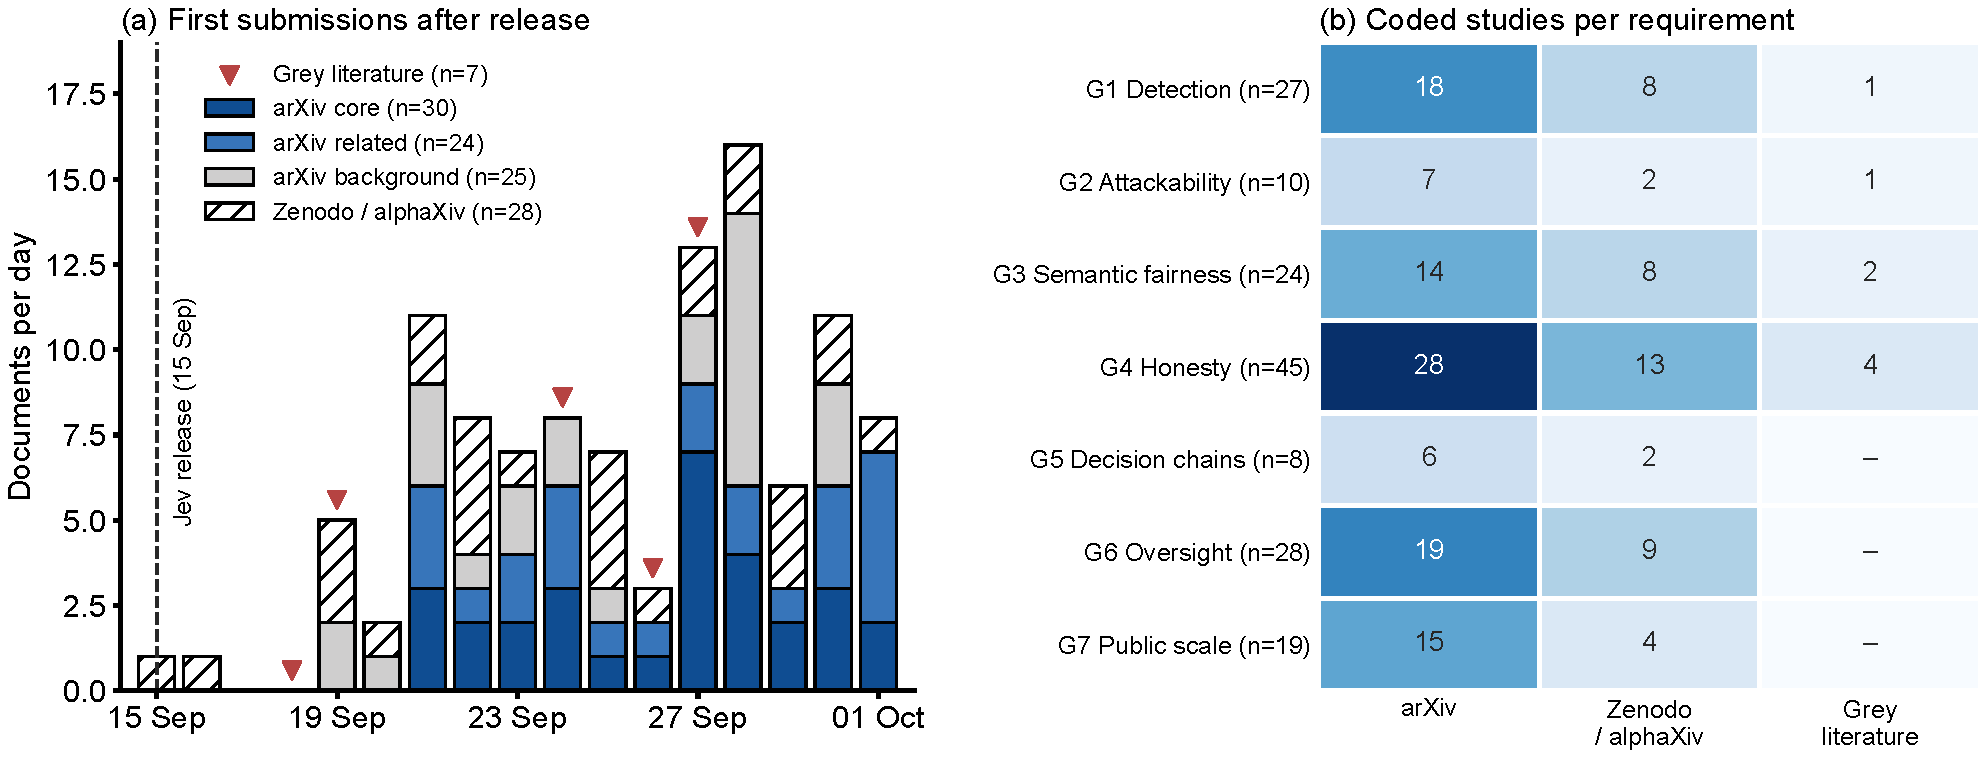
\includegraphics[width=\linewidth]{figures/fig_corpus.pdf}
\caption{证据基础。（a）\jev{}发布后每日的首次投稿：arXiv 论文按层级显示，Zenodo 和 alphaXiv 记录以阴影线表示；三角形标示灰色文献来源。（b）计入计数的已编码研究--要求对，按要求和来源划分；中间一栏含 44 个 Zenodo 对和 2 个 alphaXiv 对，一项研究可涉及多项要求。}
\label{fig:corpus}
\end{figure}

\subsection{数据提取与编码}

对每项研究，我们提取了实际测量的系统（托管的\jev{}、开源模型或二者兼有）、模型版本、任务、数据及其语言、样本量、对照、附有定位信息（节、表或图）的主要结果，以及作者本人陈述的局限。
每篇 arXiv 或 alphaXiv 研究被划入一个层级（\emph{核心}：与某项要求直接相关；\emph{相关}：补充证据；\emph{背景}：工程或其他领域，仅当其报告了与某项要求相关的测量时才予以编码）。
随后，按照对称编码手册（\cref{app:codebook}）对每个“研究--所涉要求”对进行编码，且一律针对\cref{sec:intro}所定义的\emph{检测器}用途：
若主要结果显示类型化模型履行该功能的表现至少与其对照相当，或达到研究自身设定的标准，且无需研究额外附加条件，则编码为\emph{支持}（S）；
若结果显示模型未能履行该功能，或明显逊于其对照，则编码为\emph{不支持}（N）；
若结果不一，或取决于某一附加条件，例如本地拟合的阈值、重新校准、语言或领域限制或人工审查，则编码为\emph{有条件}（Q）。
构成某项要求之检验本身的条件，例如 G2 中的对抗性内容或 G3 中的名称与顺序扰动，不属于附加条件。
对每个已编码的对，我们还记录了类型化模型在该要求上与任何生成式对照的比较结果（更好、相近、更差、不一或无）。
由于各研究的任务、指标和设计不同，我们不合并效应量；综合采用结构化叙述方式，并按 SWiM 指南~\cite{campbell2020swim}所述，对每项研究主要结果的方向进行计票。
编码、附定位信息的理由以及对照比较字段发布于 \nolinkurl{data/evidence_coding.csv}，并列于\cref{app:evidence}；编码计的是研究数量，并非效应量。

\paragraph{一致性。}
第二位编码者在不知第一次编码结果的情况下，仅依据全文和编码手册，对随机抽取的 \nKappaN{} 个研究--要求对进行了编码。
S/Q/N 编码的一致性为 \nKappaAgree{}（Cohen's $\kappa = \nKappa{}$，自助法 95\% CI \nKappaLo{}--\nKappaHi{}）；样本中第一位编码者的编码为 \nKappaMarg{}，因此该样本更多反映的是 Q 与其他编码之间的边界，而非 S 与 N 之间的边界。
两位编码者均为同一模型家族的 AI 智能体，这可能抬高一致性。
四处分歧通过重读原文得以解决，另有一项编码在审查后被修订；所有处理结果均记录于 \nolinkurl{data/coder_agreement.csv} 和 \nolinkurl{data/evidence_coding.csv}。

\subsection{质量评价与确定性}
\label{sec:appraisal}

每项已编码研究按三项条目进行评价：独立性（独立、作者评估自己构建的系统，或与厂商有关联）；设计（预注册；留出评估、交叉验证或重复运行；单次运行；案例研究；非实证）；以及是否报告了样本量和不确定性。
若研究为预注册或留出设计、报告了样本量并附区间或检验，\emph{并且}所评估的系统非作者自建，则评为\emph{设计较强}；若为单次运行、案例研究或非实证，或既未报告样本量也未报告不确定性，则评为\emph{设计较弱}；其余情形评为\emph{中等}，例如报告了样本量但未给出区间的留出研究。
在 \nAppraised{} 个经评价的来源中，\nStronger{} 个为较强，\nModerate{} 个为中等，\nWeaker{} 个为较弱（\nolinkurl{data/quality_appraisal.csv}）。
所有来源均未经同行评审；这一点对所有来源同等适用，因此不作为评级依据。

对于写入摘要或结论的每项发现，我们参照 GRADE~\cite{guyatt2008grade}的思路评定了证据的确定性。
GRADE 将非随机证据的起点定为\emph{低}；基准评测属于非随机证据，我们沿用这一起点。下述降级与升级规则是我们针对单模型基准研究所作的调整，并非 GRADE 本身的组成部分。
若某项发现仅依据单项研究、所依据的研究均非设计较强（例如两项中等研究），或在论断涉及托管\jev{}或一般类型化模型时仅依据开源模型证据，则评为\emph{极低}；若至少两项研究方向一致且其中至少一项设计较强，则评为\emph{低}；若至少三项彼此独立的设计较强研究方向一致，且其中至少一项为预注册或经独立重复，则升为\emph{中等}。包含多个分句的发现，取其各分句中的最低评级。
一项研究只有在以下条件下才计为\emph{独立重复}：其作者与原研究不同；使用自己的数据或重新实现，而非在原数据上重跑原代码；且其设计至少为中等（在原数据上重跑原代码属于再现）；在上述计数中，有共同作者的研究计为一项研究。
每项发现都有其范围，见\cref{tab:keyfindings}：托管\jev{}、开源模型，或一般类型化模型（二者兼有）。证据按系统组计数：同时测试了托管\jev{}与开源模型的研究包含一个托管组和一个开源组，其支持还是反对某项发现，依据被计数的那一组的结果判断。对于关于托管\jev{}或一般类型化模型的发现，评级仅根据托管模型证据计算，即托管\jev{}的研究以及混合研究的托管组；开源模型证据（开源模型研究以及混合研究的开源组）可以佐证此类发现，但不能提高或降低其评级，也不能使其评级有争议。对于关于开源模型的发现，评级根据开源模型证据计算。
这些规则同样向下起作用。若某项研究针对发现所指的系统和情境、就发现所陈述的结果报告了方向相反的结果，则该研究为该发现的\emph{相反研究}；在该结果上兼有两个方向结果的研究，按其主要结果所在的一方计入；超出论断范围的结果，例如论断所指以外的系统、其他结果或论断所排除的情境，既不支持也不反对该发现。
研究按设计评级排序（较强高于中等，中等高于较弱）；在同一评级内，预注册或经重复的研究排在其他研究之上。
任何相反研究都会使该发现被标记为\emph{有争议}；若最强的相反研究的排序不低于最强的支持研究，评级还会下降一级。
对于有关升级的发现，若在同一研究中、在检验升级的任务上，第二阶段比第一阶段更准确，则第二阶段计为\emph{更强的推理模型}；若差异处于抽样误差范围之内，或各准确率指标的方向相反，则视其为同级。
我们将这些规则应用于每一项发现，并纳入所有与之相关的已编码研究，而不仅限于为其引用的研究。凡在某项发现所涉要求上编码的研究，均按系统组列为支持、相反、佐证或不在范围内，并附理由，见 \nolinkurl{data/certainty_evidence.csv}；评级由 \nolinkurl{scripts/rate_certainty.py} 根据该文件与设计评级计算得出，该脚本还核查\cref{tab:keyfindings,tab:certchanges}中列出的评级与其输出是否一致。
\cref{tab:keyfindings} 的最后一个评级行是对照比较编码的计数，而非一组研究，属于描述性内容：该规则不适用于它；我们依判断将其评为低，因为对照比较字段只编码了一次，其一致性未经测量。

这些规则并非最初所采用的规则。10 月 4 日的评级只计入被引用的研究，且该规则无法降低任何评级。该规则在第 12--15 轮审查期间、即更新研究完成编码之后被修订，起因是审查者指出它只能向上起作用、未定义相反研究，且只计入被引用的研究；随后，所有发现均以修订后的规则、基于主窗口与更新检索的全部已编码研究重新评级。由于更新方案冻结了主窗口评级（\cref{sec:search}），这构成对该方案的偏离，\cref{tab:keyfindings} 同时列出 10 月 4 日的评级与当前评级。
10 月 4 日一栏列出的是当日给定的评级。若以当前规则、基于当日引用的研究重新计算，其中一项将为极低（注~$a$）：“预先设定的阈值在新数据上达不到错误目标”当时被评为中等，原因在于为其引用的四项研究中有两项（包括唯一一项预注册研究）测试的是开源模型，第三项在一个数据集上达到目标、在另一个数据集上未达到（\cref{sec:certainty-detail}）。与当日给定的评级相比，一项发现由极低升为低，一项由中等降为低，四项新被标记为有争议；没有发现达到中等确定性，其余评级不变（\cref{tab:certchanges}）。

\subsection{评审者与工具}

本分析由一位作者完成，并大量使用 AI 智能体（所有智能体角色均为 Anthropic 的 Claude Opus 5.5）。
AI 智能体执行了检索，筛选了标题和摘要，从全文中提取数据并附定位信息，提出并应用编码，评价研究质量，担任盲法第二编码者，并由同一模型的新智能体在独立的审查轮次中将正文数字与其来源进行核对；给予智能体的指令、其发现及处理结果均随数据一并发布。
作者确定了研究问题和各项要求，制定了编码手册和判定规则，并对本文的每一项判断负责；在本次发布前，作者未亲自重新编码或逐一复核各项编码。
没有任何人工进行重复筛选、提取或编码，因此未满足 Cochrane 关于由两名人员对至少五分之一记录进行双重筛选的建议~\cite{garritty2021cochrane}。

\subsection{相对于早期发布的变更}

本研究未事先撰写或注册方案。
早期基于摘要的数据集发布~\cite{survey01}未使用编码手册；本分析以全文阅读、对称编码手册、盲法第二编码者、质量评价与确定性评级以及重新执行的 arXiv 检索取而代之，并将一篇未测量任何类型化模型的论文重新归类为背景文献。

\section{按要求分述的证据}
\label{sec:evidence}

各小节先给出简要回答及该要求的编码计数，再介绍起决定作用的研究，并将发现与已有工作相联系；建议汇总于\cref{sec:design}。
“\jev{}”指托管模型；凡研究报告了版本，其版本为 \texttt{jev-1.13}，未报告版本的研究另行标注。
开源模型均标明名称。
标有 \zmark{} 的来源为 Zenodo 记录，标有 \gmark{} 的来源为灰色文献；所有来源均经全文阅读。
\Cref{fig:framework} 汇总各项编码，\cref{tab:keyfindings} 汇总各项发现及其确定性，\cref{app:evidence} 列出全部已编码研究。

\begin{figure}[t]
\centering
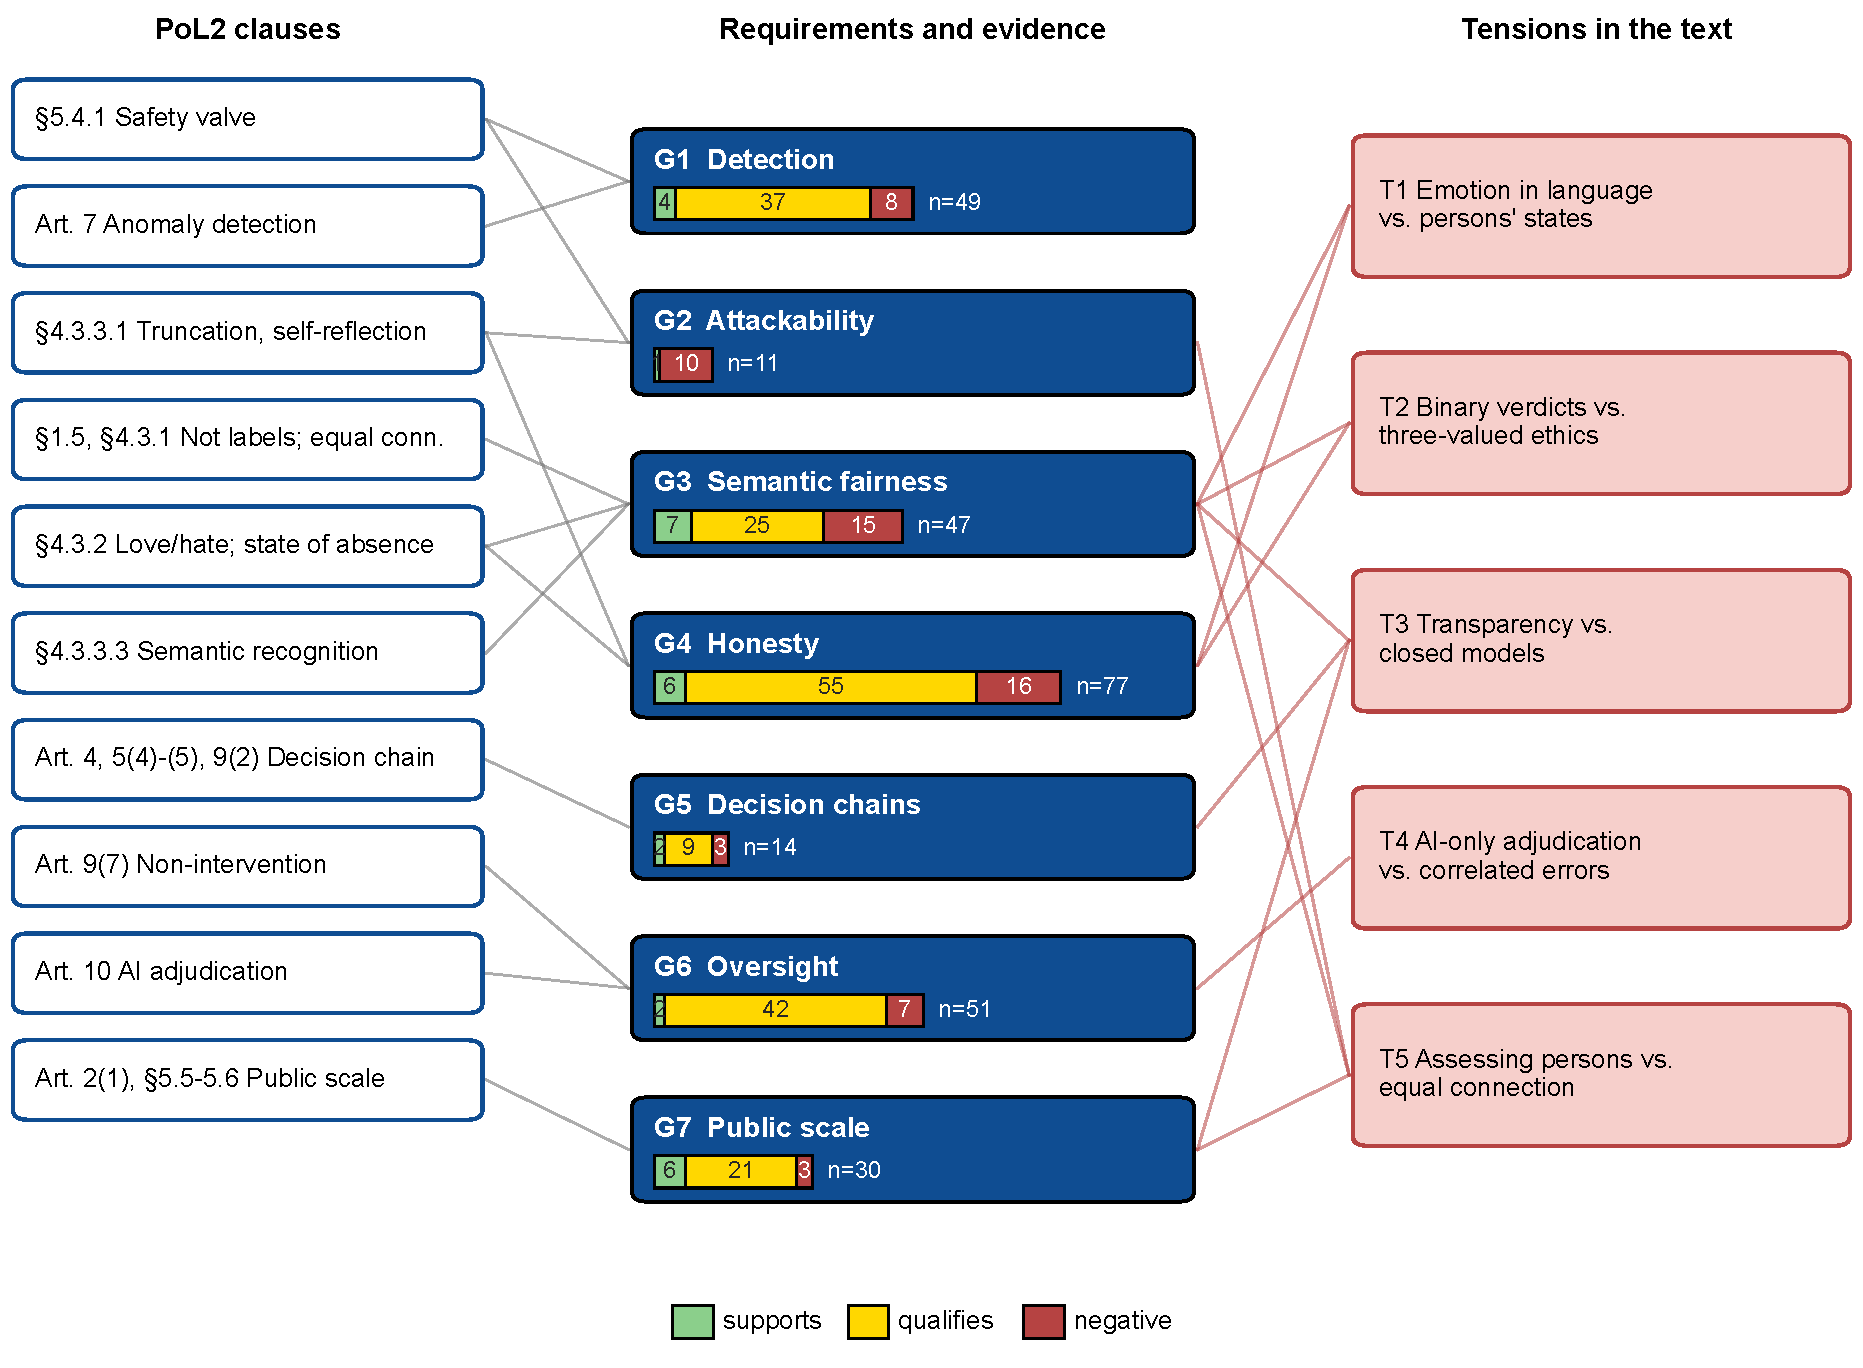
\includegraphics[width=0.95\linewidth]{figures/fig_framework.pdf}
\caption{从条款到张力。左：要求或约束机器判断的 \pol{} 条款。中：七项要求，以及为各要求提供依据的研究在检测器用途上的编码（支持、有条件、不支持；\cref{app:codebook}）；条形图计数的是研究数量，不衡量效应量或确定性，非实证文献不计入。右：\cref{sec:synthesis} 的五项张力，与其所引证据对应的要求相连。}
\label{fig:framework}
\end{figure}

% ---------------------------------------------------------------------------
\subsection{G1——类型化保障机制能否检测违规？}
\label{sec:g1}

\begin{answerbox}
作为排序可以，作为决策尚不可以。
在英文基准上，类型化模型对有害或未对齐内容的排序效果良好，成本仅为生成式评估器的一小部分，优于低成本评估器，但常低于最佳评估器；在一种情境下拟合的阈值在另一情境下失效，且错误集中于被总体分数掩盖的子类型。
编码：S~2，Q~20，N~5；与生成式对照相比，类型化模型在 21 组配对中有 6 组更好或相近，10 组不一，5 组更差。
\end{answerbox}

\paragraph{零样本排序。}
\emph{Just Ask Jev}~\cite{arx29429} 在 44 个基准、7{,}193 个实例上，针对十类对齐失效对 \jev{}（\texttt{jev-1.13.0}）进行了基准测试。
在两类样本均存在的 31 个基准上，一个通用的是/否问题在未经训练的情况下取得了 0.886 的中位 AUROC（受试者工作特征曲线下面积；95\% 置信区间 CI 为 0.821--0.952），并在其中 25 个基准上胜过域内 TF-IDF 分类器和响应长度基线；在由 API LLM 评估器评分的 19 个基准上，其每轮成本为 0.30 美元，而后者为 18.96 美元。
针对每个基准定制问题仅使中位 AUROC 变化 $+0.006$（CI $-0.004$ 至 $+0.015$）；更重要的是向模型\emph{展示}什么，因为许多失效是相对于某一参照（如用户陈述的信念或注入的指令）来定义的。
在对托管 \jev{}、七个开源类型化模型、经训练的分类器和 LLM 的匹配比较中，\jev{} 是最准确的类型化模型，并以 AUROC 0.921 区分出不在范围内的请求，但在意图检测上，基于标签微调的小型分类器胜过它（0.940--0.948 对 0.913）~\cite{arx00346}。
在七项公开的审核、幻觉、推理和注入任务的共享样本上，\jev{} 在全部六项二分类任务上的 AUROC 均为低成本生成式评估器中最高，但一个成本为其 42--97 倍的前沿模型在七项中的两项上胜过它~\cite{zen22885291}\zmark{}。与最强的生成式评估器相比，它往往准确性较低：在 15 项预注册的社会科学标注任务中，它有 14 项落后于最佳 LLM，macro-F1 的中位差距为 11.6 个百分点~\cite{arx24574}；在合同推理上，其准确率（77.38\%）低于全部七个托管 LLM 的点估计，但并非显著低于每一个，且成本最低~\cite{arx27678}。在智能体轨迹上，其正类 F1（精确率与召回率的调和平均数）为 77.8，而最强生成式评估器为 74.1，但其精确率较低，且在四个基准中的两个上胜出（版本未报告）~\cite{arx34862}。

\paragraph{阈值不可迁移。}
在 \emph{Just Ask Jev} 中，中位 F1 从默认阈值 0.5 下的 0.706 升至交叉验证阈值下的 0.822；增益主要来自采用规则或评估器评分标签的基准，而在经人工验证的标签上，默认阈值表现相当（0.721 对 0.694）~\cite{arx29429}。
另一团队的再现研究在 \texttt{jev-latest} 别名上重新运行了作者的代码和数据，覆盖其 44 个基准中的五个（与原文的中位绝对差为 0.0036），并发现了极端情形：在 TensorTrust 劫持任务~\cite{toyer2024tensor}上，AUROC 为 0.95，但 F1 在阈值 0.5 下为 0.158，在经二折交叉验证选定的阈值 0.35 下为 0.947；其拟合的五个阈值中没有一个是 0.5~\cite{jkf87_2026replication}\gmark{}（\cref{fig:fragility}a）。
在一项语义数据库工作负载中，固定阈值 0.5 下的 \jev{} 平均 F1 为 63--66\%，按谓词不同从 24\% 到 89\% 不等~\cite{arx02046}。
对一个领域的拟合可能以另一领域为代价：一个基于中文合规查询微调的开源 Laya 护栏，在其自身测试划分上将良性误报率从 35.71\% 降至 0.42\%，但在一个通用中文安全基准上准确率下降（60.33\% 降至 56.81\%），除非在微调中回放早期数据~\cite{arx33671}。

\paragraph{总体指标掩盖集中的失效。}
在智能体安全筛查中，\jev{} 在三项任务中的两项上是最强的类型化模型（交互风险 AUROC 0.961，Laya 为 0.533），但它漏掉了\emph{全部} 130 条不含显式指令的提示注入，对每一条给出的不安全概率均低于 0.1；它在该基准上的 167 次漏检中有 130 次发生在置信度 $\geq 0.95$ 时~\cite{arx33401}。
一个开源 Laya 评估器在答案被显式陈述时近乎完美，但在需要察觉某事物\emph{缺失}时降至 0.31，而一个生成式评估器在相同条目上得分 1.00~\cite{zen22901853}\zmark{}。
在警方交通事故叙述中，\jev{} 在正则表达式标记的分层内几乎完美地识别出有记录的妊娠，但在低流行率分层中，42 个经裁定的阳性中仅有 14 个得到确认，因此在一个分层中测得的错误率不能推及另一分层~\cite{arx00213}。

\paragraph{证据并非文本时。}
在数值型网络流特征上，零样本 \jev{} 的得分低于始终预测多数类（9.8\% 对 22.8\%），即使在上下文中提供 150 个带标签样例，也仍远低于基于标签训练的小型树模型~\cite{arx00376}。
在一个较陈旧的入侵检测基准上，每类提供一个带标签样例时，它的 F1 达到 0.856，略低于一个生成式对照（0.880），每次运行约有 43 次误报，而在每类同样仅一个样例的条件下，随机森林约为 764 次（每类八个样例时，随机森林的 F1 略高）~\cite{arx01079}。
在一项供水管网筛查中，它与专家规则树相当（macro-F1 0.63 对 0.59），并在训练时留出的事件子类型上胜过一个监督分类器，但仍低于完全监督模型和两个前沿 LLM~\cite{arx02048}。

\paragraph{与已有工作的关系。}
这些结果在类型化模型上重现了读取概率的安全分类器的已知特性~\cite{inan2023llama,markov2023holistic}：排序良好，阈值难以迁移，失效集中于子类型~\cite{rottger2021hatecheck}。
静态分数也会过时：在英文中，将一个词替换为含义相同的新近造词，使 20 个零样本模型中有 6 个对超过 10\% 的句对翻转了仇恨言论标签，且多数模型对较晚年份仇恨帖子的检测效果较差~\cite{dibonaventura2025hatevolution}。
新的是价格：对每条消息进行排序如今已廉价到足以成为默认做法。

% ---------------------------------------------------------------------------
\subsection{G2——受审内容能否操纵保障机制？}
\label{sec:g2}

\begin{answerbox}
能。
凡以待判内容攻击类型化模型的研究，均发现攻击取得了一定成功，且有效的攻击未必看起来像攻击：一条插入的观点、流畅的背景文本或一个词汇诱饵；唯一被编码为支持的研究发现，注入很少选中攻击者的目标，而针对 \jev{} 的其他攻击使这一发现有争议（\cref{tab:keyfindings}）。
在同一研究中受到攻击的其他系统同样易受攻击。
编码：S~1，Q~0，N~9；这是编码最一致地为不支持（N）的要求。
\end{answerbox}

\paragraph{注入与插入内容。}
在 510 个重构的 InjecAgent 案例上，恶意内容改变了 \jev{} 的动作概率，但仅在 9 个案例（1.8\%）中选中攻击者的目标；“ignore previous instructions”（忽略先前指令）标记反而\emph{削弱}了效果，利用分数反馈的自适应攻击者在新调用上达到 3.5\%（510 中的 18 个；CI 0--10\%）~\cite{arx28613}。
\emph{JevOut}~\cite{arx30243} 利用模型自身的概率，在 64 次被接受的查询内搜索简短流畅的上下文附加内容，这些内容受约束且经另一模型核查，以保持问题和正确答案不变；它们将 508 个初始正确的 \jev{} 决策中的 312 个（61.4\%）引导至攻击者选定的错误选项，而另外三个决策系统（包括一个基于 Qwen3-1.7B 构建的类型化接口）在其各自的正确决策上有 64.9--73.2\% 被引导（\cref{fig:fragility}b）。
在 \emph{JevAdvBench}~\cite{arx31142} 中，在状态后附加一条未经核实的观察者观点，即翻转了 \jev{} 12.1\% 的决策（CI 8.5--15.5），与冒充权威（最强的注入指令）在统计上持平，尽管该指令须置于问题中，而观点只需置于状态中；对问题的良性改写所引起的变化处于重复运行噪声范围之内。
当正确动作需要一个未明示的推理时，状态中与某一选项呼应的词语会起到诱饵作用：在一个家务任务基准的误导性步骤上，\jev{} 的正确率为 36\%，选择诱饵的比例为 56\%~\cite{arx01834}。
与问题无关但主题相关的段落使其问答准确率从 0.84 降至 0.75，而其置信度保持在 0.83~\cite{arx01006}。

\paragraph{自适应与伪装攻击。}
针对一个基于 \jev{} 的尽职调查应用（版本未报告）运行的三个多轮自适应攻击智能体中，最强者在 27 次运行中成功 25 次，平均在第四轮得手，而将内容标记为不可信并无实质影响；作者称其为针对单一应用的方向性研究~\cite{checkpoint2026jev}\gmark{}。
在一项预注册的供水管网研究中，设计成看似正常运行的攻击是最难识别的一类（召回率 0.34），在一个相似样本集上，被一致性门控接受为良性的 76 个窗口中有 21 个是攻击~\cite{arx02048}。
在开源的 \jev{} 兼容模型 Kev-0.8B 中，多问题调用里一条植入的注释即可同时改变若干治理答案~\cite{zen23038928}\zmark{}。

\paragraph{与已有工作的关系。}
这些是提示注入和对抗优化~\cite{perez2022ignore,greshake2023not,zou2023universal}在类型化模型上的实例。
类型化模型特有的一点是，使其有用的概率向量同样为攻击者提供指引：有概率反馈时成功率为 63.6\%，仅有标签时为 56.4\%，但没有概率反馈时攻击也能奏效~\cite{arx30243}。

\begin{figure}[t]
\centering
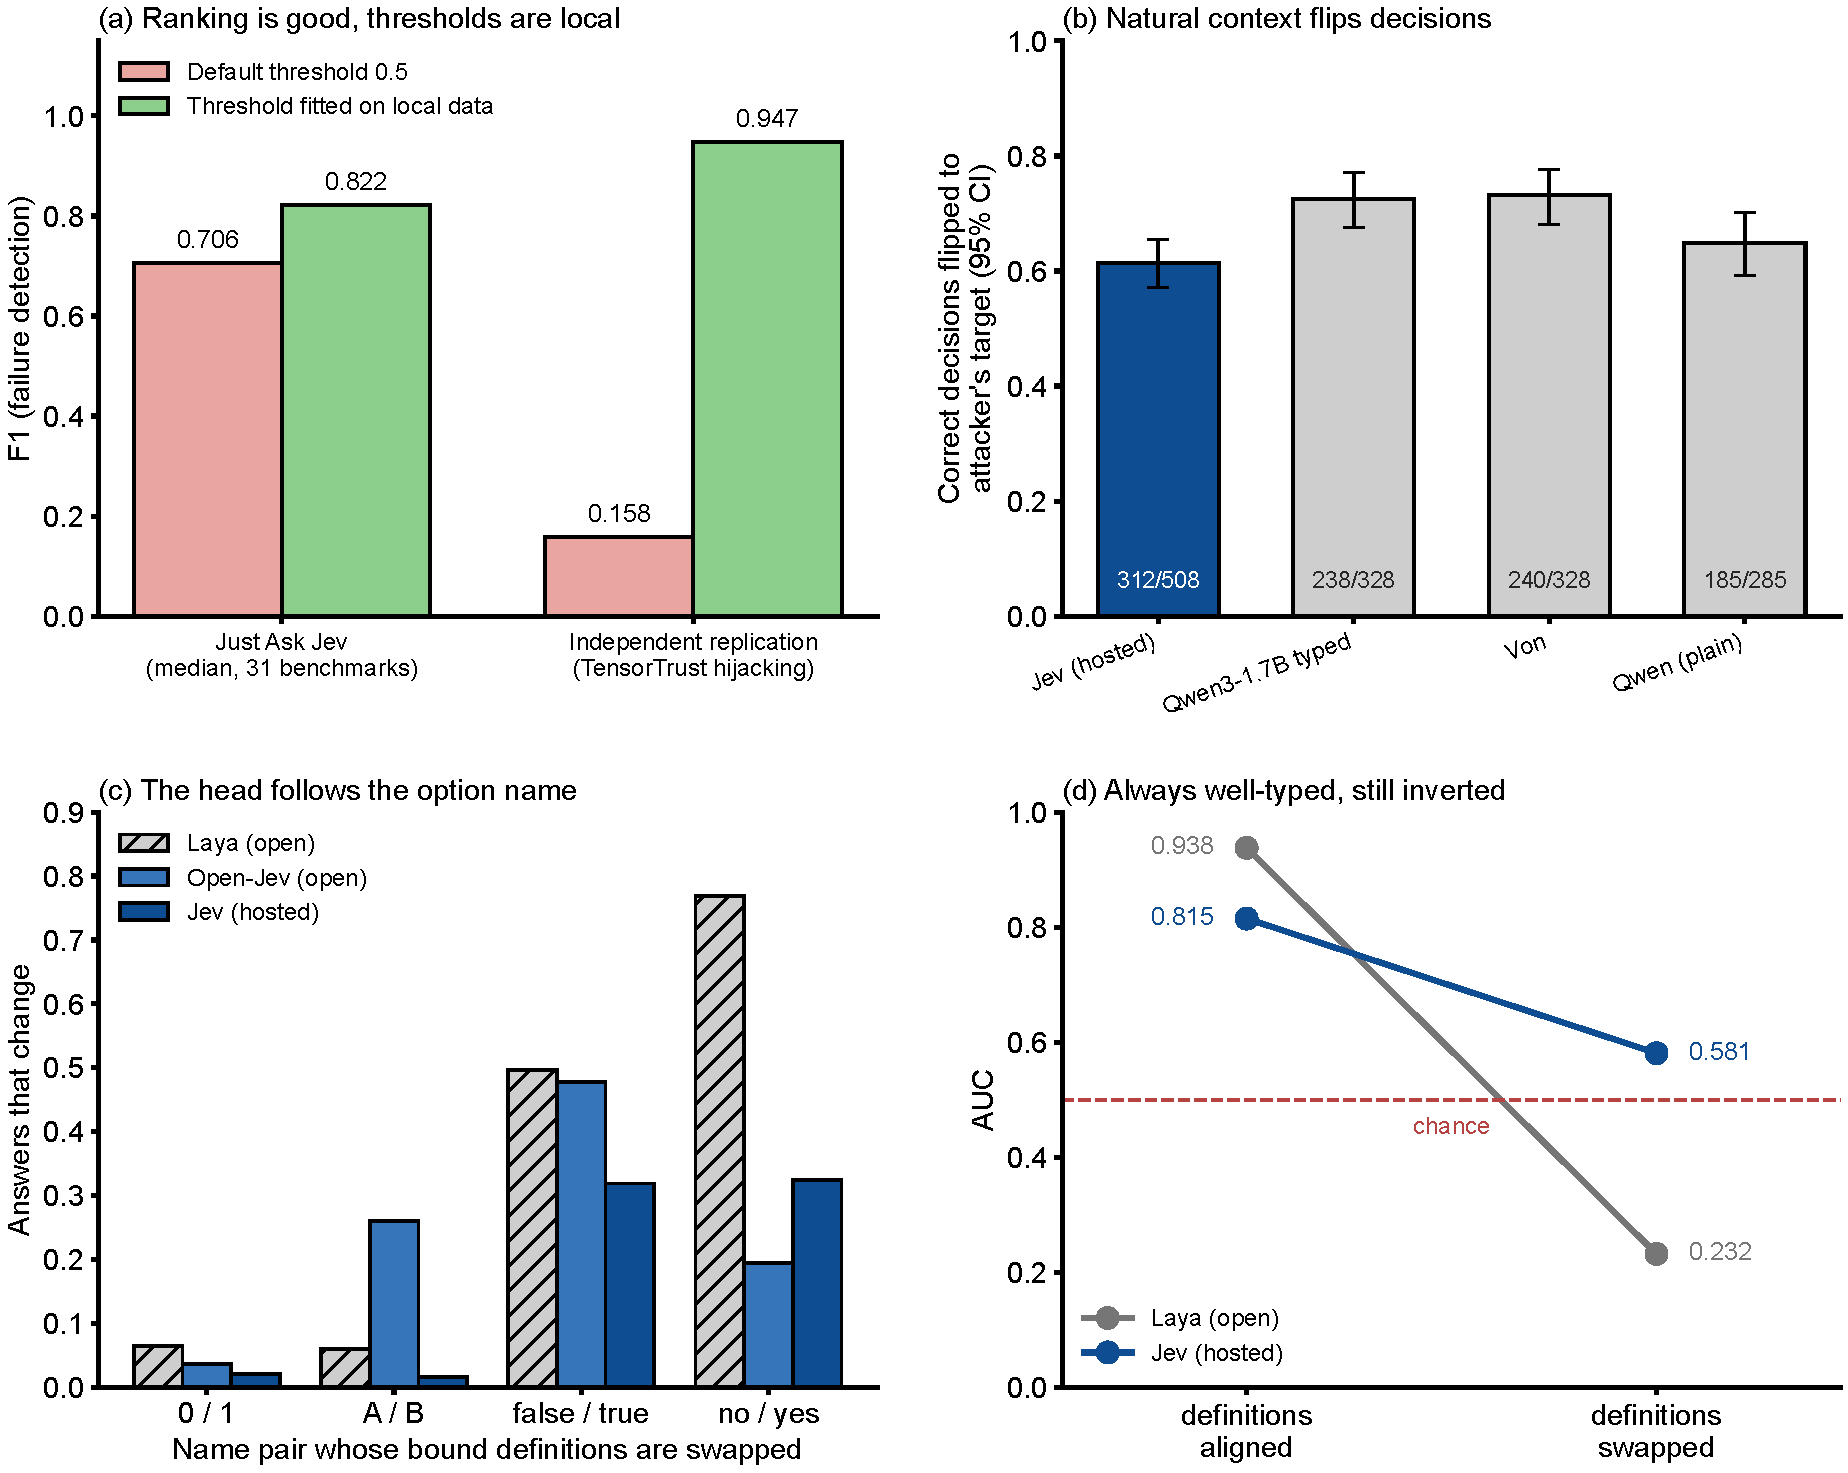
\includegraphics[width=0.9\linewidth]{figures/fig_fragility.pdf}
\caption{G1--G3：一个检测器，而且是脆弱的检测器。
(a) 默认阈值下的 F1 与基于本地数据拟合的阈值下的 F1~\protect\cite{arx29429,jkf87_2026replication}。
(b) 经优化的流畅上下文附加内容将初始正确决策引导至攻击者选定的错误选项的比例，各系统均以其自身的正确条目计；“Von”是该研究所评估的一个开源类型化模型；误差线为根据所报告计数计算的 Wilson 95\% 区间~\protect\cite{arx30243}。
(c) 在问题、状态、名称和定义文本均不变的情况下，交换绑定于一对选项名称的定义后发生变化的答案比例；Open-Jev 基于 1{,}800 个问题，Laya 和 \jev{} 基于 1{,}200 个问题~\protect\cite{arx26758}。
(d) \texttt{yes/no} 定义与名称对齐或互换时的 AUROC；类型错误率始终为 0\%~\protect\cite{arx26758}。
(a) 和 (b) 使用 \texttt{jev-1.13.0} 或 \texttt{jev-latest} 别名；(c)--(d) 所涉研究未报告托管版本。}
\label{fig:fragility}
\end{figure}

% ---------------------------------------------------------------------------
\subsection{G3——语义判断是否稳定且公平？}
\label{sec:g3}

\begin{answerbox}
默认情况下并非如此。
决策可能跟随选项名称而非绑定于其上的定义，取决于顺序和措辞，并偏向某一种文化的价值观；中性的选项标识符和选项轮换可消除其中很大一部分。
稳健性因模型而异：托管 \jev{} 受影响程度低于 Laya，但高于某些更大的开源解码器。
编码：S~2，Q~10，N~12。
\end{answerbox}

\paragraph{选项名称可能压过定义。}
\emph{Type-Safe Is Not Error-Free}~\cite{arx26758} 固定问题、状态、选项名称和定义文本，仅交换哪个定义绑定于哪个名称。
对 Laya 而言，交换绑定于 \texttt{yes} 和 \texttt{no} 的定义改变了 76.9\% 的答案，而对 \texttt{0} 和 \texttt{1} 仅为 6.5\%，其 AUROC 从 0.938 降至 0.232，这种反转是类型检查无法发现的；托管 \jev{}（版本未报告）改变了 32.5\% 的答案，约为其重测下限的 24 倍，其 AUROC 从 0.815 降至 0.581（\cref{fig:fragility}c--d）。
在匹配的测试框架下，针对固定评分细则的同样交换使 \jev{} 1.13.0 每 100 个答案中翻转 50.5 个（下限 1.3），而数字或随机字符串标识符使其接近下限；Laya 翻转 91.3 个，四个更大的开源解码器翻转 4.2--6.5 个~\cite{arx00346}。

\paragraph{顺序、措辞与文化。}
在 ANLI 上，尽管选项位置是平衡的，\jev{} 仍将 38.8\% 的预测和 51.3\% 的错误落在“neutral”（中立）选项上；在六个数据集上，同一组有序选项的两种随机排列在 74.4\% 的条目上一致~\cite{arx38827}。
在 20 个选项的任务上，倒转选项列表使开源 LLM 的类型化读出约三分之一的答案发生变化，对多种轮换取平均可将其降至 14--18\%~\cite{arx00831}；对 \jev{} 而言，在某一基准所测试的科目上，轮换选项未改变准确率~\cite{arx37647}。
在道德困境上，\jev{} 在多次运行间保持稳定，但改写措辞使其答案变化大得多~\cite{zen23023694}\zmark{}。
当以群体间强制选择的形式提问时，在八项特质中“White”（白人）占 \jev{} 首选的 51\%，尽管对直接的优越性主张，它通常以约 3\% 的“yes”概率予以否定；这项单一的非正式测试（版本未报告）未对选项顺序进行平衡~\cite{simmons2026saidno}\gmark{}。
在无人设时，\jev{} 回答跨文化价值观调查的方式与其自身的美国人设相似；沙特人设在英文中重现了人类沙特--美国差异的 87\%，在阿拉伯文中则为 62\%~\cite{arx36399}。
在一项研究中，论证由谁提出对 \jev{} 影响甚微，但它所用的评分细则与对话模型不同，因此本文未将其与后者排名比较~\cite{arx35286}。

\paragraph{语言。}
TypeSafe 称，英语以外的语言（包括中日韩文字）“handled but not equally well”（可处理，但效果不尽相同）~\cite{typesafe_models}。
一个以代码仓库形式发布的中文决策基准发现，托管 \jev{} 在中文语音路由上无需重新校准，在选项顺序互换下改变了 1.9\% 的语音路由决策（客户服务上为 2.9\%），在简体与繁体之间改变了 1.7\%（$n = 323$），而开源 Laya 多语言模型的选项顺序变化率为 10.8\%（语音路由）和 20.6\%（客户服务）~\cite{qin2026zhdecisionbench}\gmark{}。
在第二个中文基准上（由以 Laya 为初始化的中文模型的作者构建），托管 \jev{}（版本未报告）在通用任务上的校准误差为 11.45\%，而作者的通用模型为 3.78\%，后者准确率也略高于 \jev{}；其经领域微调的专用模型在医学上胜过 \jev{}，但在各专业领域的平均准确率为 \jev{} 的 92\%，且在这些领域校准更差（12.08\% 对 5.57\%）~\cite{arx36965}。
在一项基于印度英语方言文本的预注册测试中，\jev{} 的校准在 22 个模型中最佳（ECE 0.063），但仅限单一任务~\cite{arx24574}。在一个包含 37 个数据集的基准中，全部三个模型（类型化与生成式）在低资源语言上均出现性能下降~\cite{arx37647}。

\paragraph{与已有工作的关系。}
选项顺序和标签敏感性在 LLM 与 LLM 评估器中早有记载~\cite{zhao2021calibrate,pezeshkpour2024large,zheng2024large,wang2024fair}；类型化输出并未消除这一问题，名称--定义反转是其更尖锐的形式。
群体与文化方面的结果呼应了在仇恨言论分类器~\cite{sap2019risk,davidson2019racial}和标注者~\cite{sap2022annotators}中发现的偏差。

% ---------------------------------------------------------------------------
\subsection{G4——概率是否诚实，“不足”是否会被报告？}
\label{sec:g4}

\begin{answerbox}
部分如此。
托管 \jev{} 在熟悉的封闭选择任务上通常校准良好，一般优于生成式模型的自述置信度，与前沿模型相比则结果不一；但校准是局部的，相关概率并不总是一致，显式的“I don't know”（不知道）选项在其为正确答案时很少被选中，“none”（以上皆非）的选择也不一致。
另设一个关于证据是否充分的是/否问题，检测信息缺失的效果优于置信度（在一项研究中 AUROC 为 0.95 对 0.85），但其筛选答案的效果较差。
编码：S~3，Q~29，N~13；与生成式对照相比，类型化模型在 18 组配对中有 9 组更好，2 组更差。
\end{answerbox}

\paragraph{在熟悉任务上经过校准。}
本文语料库中覆盖面最广的基准包含 37 个数据集上的 346{,}009 次请求，发现 \jev{} 在 27 个数据集上比一个开源 27B 模型更准确（其中 11 个区间不重叠），且合并计算时在 Choice 问题上校准良好（期望校准误差，ECE，0.028；未加权均值 0.061），其置信度可支持选择性作答~\cite{arx37647}。
一项博客测试在 3{,}066 个词义语境对上，于提示针对该数据集调优后测得 ECE 为 0.027~\cite{grazian2026calibrated}\gmark{}。在一项涵盖 575{,}442 次调用的受控审计中，\jev{} 在熟悉的封闭选择任务上的平滑校准误差为 0.015--0.033~\cite{arx01006}。
其标注置信度的校准优于 19 个 LLM 中 16 个的自述置信度，但三个前沿模型的中位误差更低，且区间重叠（0.066 对 0.157）~\cite{arx24574}。其他前沿比较对 \jev{} 更有利：在三个医学基准中的一个上，其概率的校准优于一个前沿推理模型（ECE 0.063 对 0.146），在另外两个上误差相近~\cite{arx34024}；在六项公开二分类任务上，其原始 Brier 分数为所有受测系统中最低，但经重新校准后，一个前沿模型的分数略低（0.071 对 0.076）~\cite{zen22885291}\zmark{}。一个由作者构建的医学类型化模型的校准误差也低于匹配的生成式基线~\cite{arx00381}。

\paragraph{校准是局部的。}
在交通事故叙述的 2{,}416 个盲法人工标签上，\jev{} 的原始概率总体偏高，将流行率高估约 80\%，且过于靠近中间值；折外重新校准将合并 ECE 从 0.0231 降至 0.0069~\cite{arx24052}。
在放射学语句上，基于留出集的重新校准将 ECE 从 0.1235 降至 0.0077，一个开源基线的改善幅度相近~\cite{arx27607}（\cref{fig:honesty}c）。
以零样本方式判断另一模型的答案是否正确时，\jev{} 无法开箱即用（ECE 0.133）~\cite{arx24881}；在 ChaosNLI 中标注者分歧最大的条目上，其 Choice 概率的 ECE 升至 0.339，而在一致性最高的四分之一条目上为 0.076，该预注册研究同时发现，它的校准远优于一个本地生成式基线，且其置信度仍能对有争议的条目进行排序（AUROC 0.744）~\cite{zen23032384}\zmark{}。在提示针对该数据集调优后，一项博客测试在 ChaosNLI 的 612 个二分 $\alpha$NLI 条目上测得 ECE 为 0.025，以全部条目上的群体比例为评分基准~\cite{grazian2026calibrated}\gmark{}。
这是分布偏移下校准的一般规律~\cite{ovadia2019trust}；这些研究之间的 ECE 数值不可比较。

\paragraph{加总不为一的概率。}
在 480 对“标签是 X”与“标签不是 X”的陈述上，\jev{} 的两个概率之和偏离 1 的平均幅度为 0.064，是其自身重复噪声的五倍（\cref{fig:honesty}a），且偏离集中于其不确定之处~\cite{arx33209}。
在 1{,}000 个合成案例中，其是/否接口与 Choice 接口在 32.8\% 的案例上导致不同的“执行或暂缓判定”决策（一个经后训练的开源模型：34.2\%）~\cite{arx37470}。
基于 738{,}164 个答案对厂商置信度公式的重构表明，填充选项集会抬高所报告的置信度~\cite{yurin2026confident}\gmark{}。

\paragraph{缺失的“不足”。}
在一个医学基准上提供“I don't know or cannot answer”（不知道或无法回答）选项时，在该选项为正确答案的 162 个条目中，\jev{} 选择了其中 17 个（10.5\%），与一个前沿生成式模型（8.6\%）相近；在“None of the above”（以上皆非）为正确答案的条目中，\jev{} 选择它的比例为 53.9\%，而同一前沿模型为 73.9\%~\cite{arx34024}。
当所列答案全部错误且识别这一点需要算术运算时，它仅在 7\% 的条目上选择显式的“None”，而在含有正确答案的条目上 99\% 回答正确；对该选项重新命名，或在清点类案例中移动其位置，几乎没有改善，而逐候选的是/否核验达到 99\%，一个推理型生成式模型能正确拒绝，在开发数据上选定的“None”概率阈值将正确拒绝率提高到 79\%~\cite{arx39496}。
在没有相关信息时，\jev{} 仍会将高达 0.80 的概率置于一个显著选项上；另设一个询问证据是否充分的问题，在多跳问题上区分完整与不完整证据的 AUROC 为 0.95，而置信度为 0.85，但作为接受答案的筛选器，其准确率比置信度低 2--6 个百分点~\cite{arx01006}。
在一项小型案例研究中，\jev{} 对冲突与无知的是/否概率落在同一区间，而一个同时列出这两种状态的 Choice 问题在全部四个案例中将二者区分开来~\cite{zen22848952}\zmark{}。
对一个开源读出进行窄域微调，压制了“none of the above”并使其偏向“yes”，而验证损失仍在持续改善~\cite{arx02076}。

\paragraph{与已有工作的关系。}
校准的局部性及其在分布偏移下的失效已有定论~\cite{guo2017calibration,ovadia2019trust,hebertjohnson2018multicalibration}，置信度与弃权之间的差距亦然~\cite{kamath2020selective,wen2025know}。
新的是如下证据：对类型化模型而言，就充分性\emph{发问}比读取置信度更能检测信息缺失。

\begin{figure}[t]
\centering
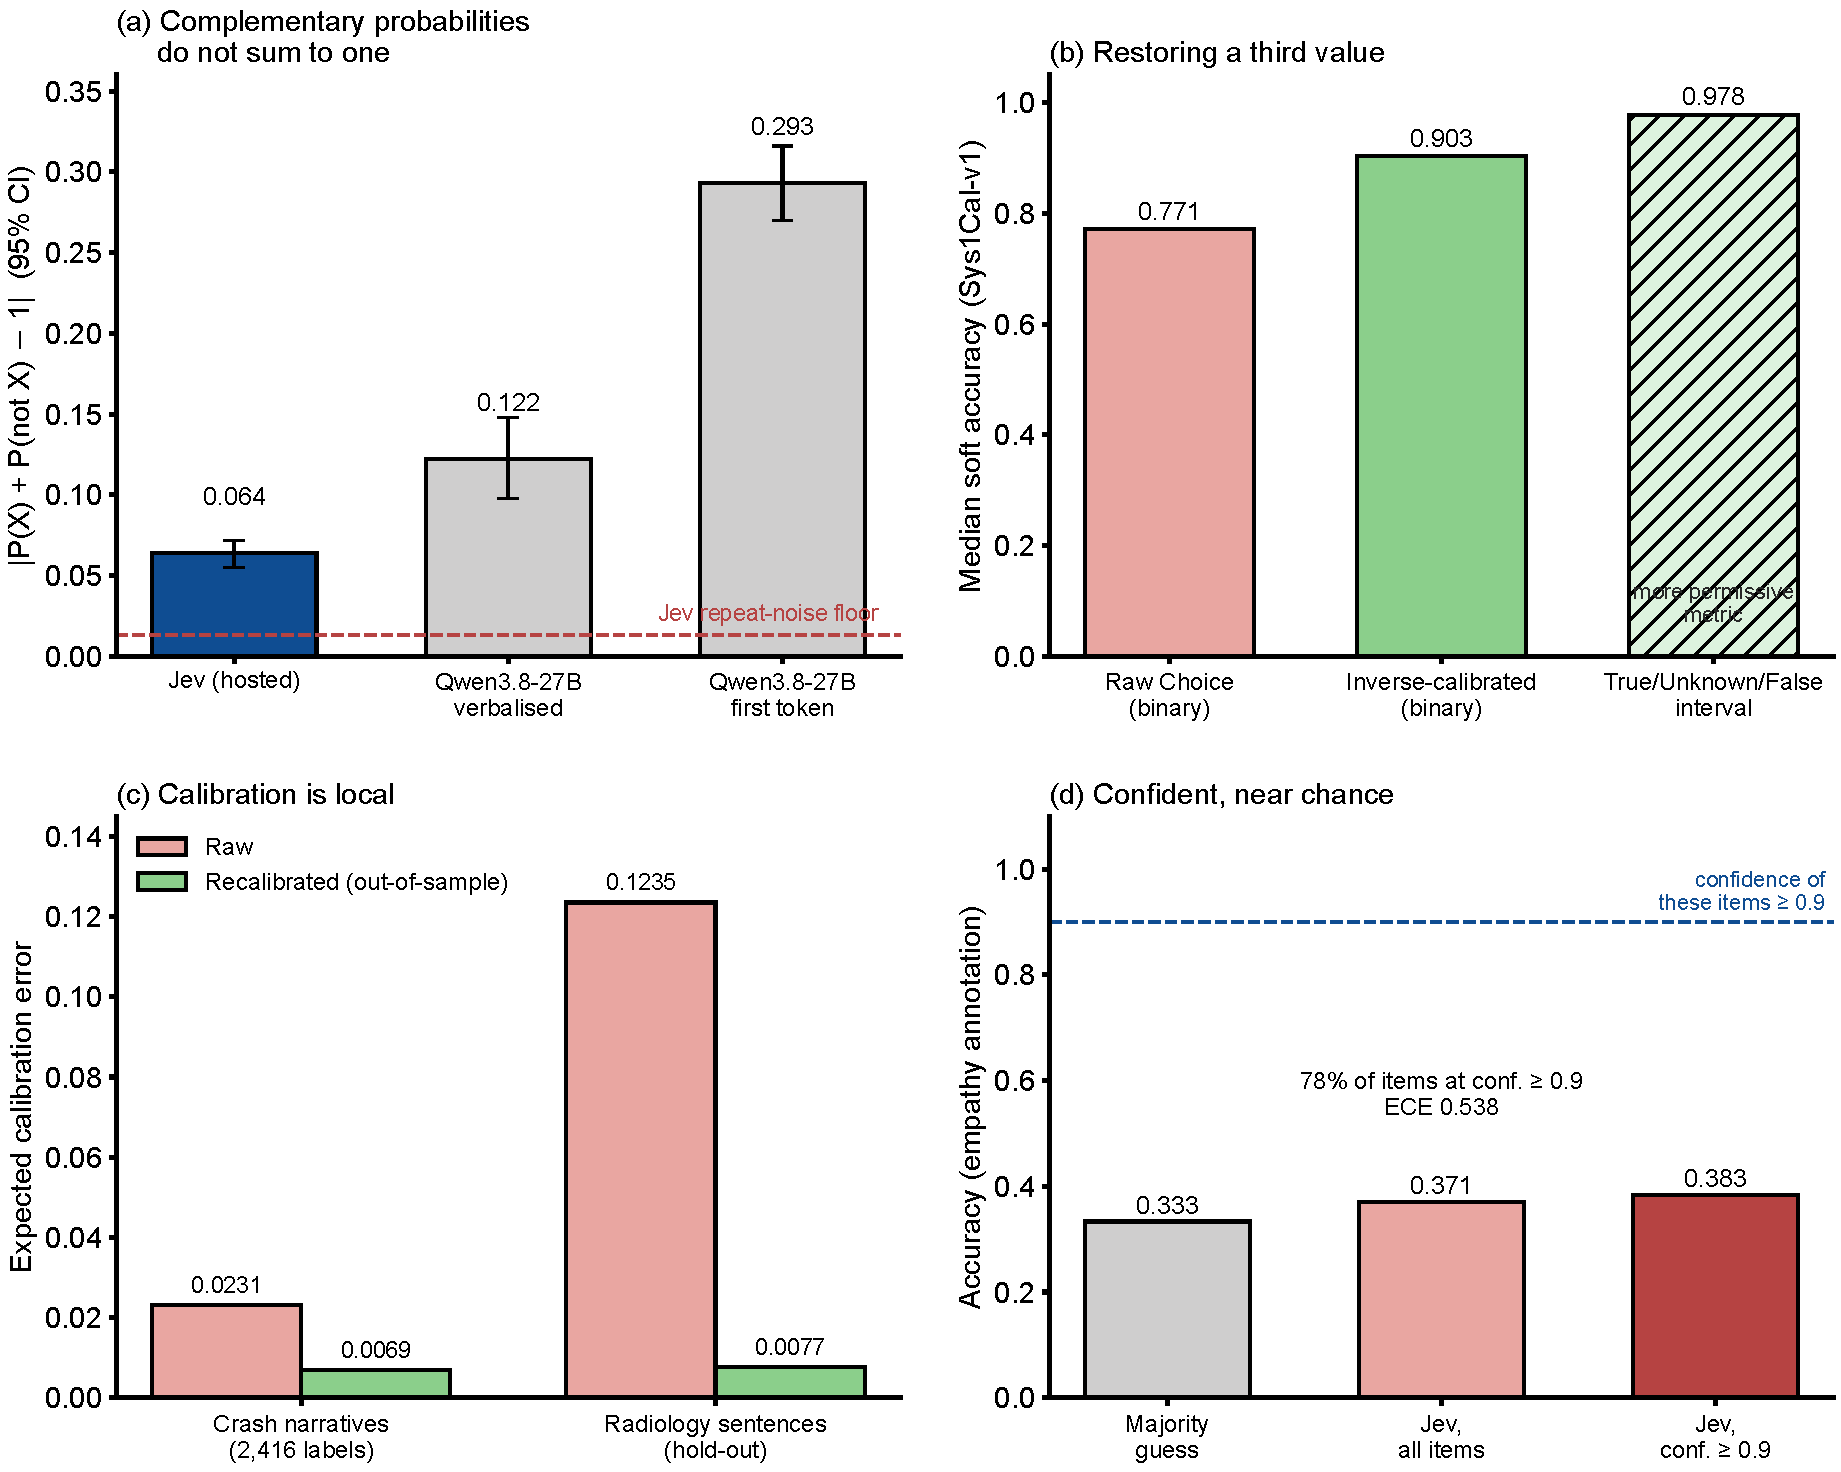
\includegraphics[width=0.9\linewidth]{figures/fig_honesty.pdf}
\caption{G4：诚实性。
(a) 480 个否定对上 $P(X)+P(\neg X)$ 偏离 1 的平均绝对偏差，与 \jev{} 的重复噪声下限对照~\protect\cite{arx33209}。
(b) Sys1Cal-v1 上的中位软准确率：原始 Choice 答案、校正被压制的“unknown”概率质量后（该研究的一个假设），以及采用更宽松的真/未知/假区间指标时（阴影）~\protect\cite{arx35342}。
(c) 基于本地标签重新校准前后的 ECE，采用折外方式~\protect\cite{arx24052}或留出集~\protect\cite{arx27607}。
(d) 共情标注（三个平衡类别）：\jev{} 在全部条目上及在其以置信度 $\geq 0.9$ 作答的条目上的准确率，与多数类基率对照~\protect\cite{arx24574}。}
\label{fig:honesty}
\end{figure}

% ---------------------------------------------------------------------------
\subsection{G5——仅为一个数值的决策能否被审计和解释？}
\label{sec:g5}

\begin{answerbox}
可以被记录和分解，但无法被解释。
类型化决策不返回理由，由多个问题或接口组合而成的决策未必一致；将中间事实作为独立步骤写入状态，可使链路可检查，且当这些事实正确时，可提高准确性，但在两项较晚的研究中，分解并未提高准确性（\cref{sec:update}）。
编码：S~2，Q~3，N~3。
\end{answerbox}

\paragraph{有记录而无理由。}
类型化模型只返回一个概率，别无其他，因此其输出中没有任何内容能表明是输入的哪一部分产生了判定~\cite{willison2026jev}。
一篇 Zenodo 评论认为，去除推理轨迹在结构上使责任归属更加困难~\cite{zen22847531}\zmark{}；另一篇认为，类型化推断可能将治理承诺转移到其开发者编写的模式、选项集、评分细则和阈值之中~\cite{zen22866847}\zmark{}。
当求解器在修改其逻辑谜题答案时被展示 \jev{} 的概率，其表现并不优于单纯再看一遍~\cite{zen22849329}\zmark{}。

\paragraph{可组合与不可组合的链路。}
在十个科学工作流中，\jev{} 正确完成了全部中间语义选择，而对照模型的七次错误选择（全部出现在同一问题上）改变了下游计数却未改变最终标签：仅凭最终标签准确率无法发现这些错误~\cite{arx24965}。
通过两种接口提问时，同一决策在 32.8\% 的案例中导致不同动作~\cite{arx37470}；由细粒度答案重构的类别概率与直接询问所得概率的平均总变差为 0.22--0.35~\cite{arx33971}；当条件发生变化时，逐步校准审计可能遗漏链路层面的错误~\cite{zen23064668}\zmark{}。
分解可以有所帮助：当 \jev{} 对对手动作的预测被写入状态时，其在误导性博弈中的决策正确率从 33\% 升至 94\%，但在给定一个错误的书面前提时，它在 26 次调用中有 24 次遵循该前提，这使书面事实本身成为审计点~\cite{arx01834}。

\paragraph{与已有工作的关系。}
决策后生成的解释未必反映产生该决策的因素~\cite{doshivelez2017towards}，而文档标准~\cite{mitchell2019model,gebru2021datasheets}描述的是模型和数据，而非单个决策；类型化保障机制需要一份决策记录，以及一份独立来源的理由陈述。

% ---------------------------------------------------------------------------
\subsection{G6——“有把握则执行，无把握则升级”是否可行？}
\label{sec:g6}

\begin{answerbox}
取决于升级的去向以及阈值的设定方式。
在若干研究中，将不确定案例升级至更强的推理模型，或仅接受经独立构建的规则确认的判定，节省了四分之一至一半以上的成本，且准确性无损失，但一项较晚的研究使这一发现有争议（\cref{sec:update}）；升级至同类模型则保留了高置信错误；在设定了预先固定阈值的研究中，多数研究的阈值在新数据上未能达到其错误目标，但在若干研究（包括一项预注册研究）中，\jev{} 的阈值达到了目标（\cref{tab:keyfindings}）。
编码：S~1，Q~23，N~4。
\end{answerbox}

\paragraph{有效的升级。}
\emph{JEV-as-a-Judge}~\cite{arx26550} 发现，在判定可直接从文本中读出的情形下，\jev{} 与 GPT-6 相差不超过三个百分点，费用仅为后者的 0.36\%，而在判定须经推导的情形下则明显落后。采用预先冻结的阈值，级联在 1{,}610 个留出配对上（83\% 来自 RewardBench；在 JudgeBench 上低 0.74 个百分点）以 GPT-6 费用的 41.4\% 超过 GPT-6 0.93 个百分点（CI 0.24--1.66），在针对两个新工作负载的前瞻性实时测试中，以各自 100 个本地标签设定阈值，它以 75.5\% 的费用与 GPT-6 持平（\cref{fig:escalation}a）。
在一项基于模拟网络数据、采用封存测试轮次的预注册研究中，仅当一个独立构建的规则树同意时才接受 \jev{} 的良性判定，使前沿 LLM 审核者得以跳过 34.5--38\% 的案例而 macro-F1 无损失，迁移至另外两个网络时亦然，但伪装攻击仍能通过（\cref{sec:g2}）~\cite{arx02048}。
一个预注册的标注级联以四分之一至一半的成本达到了仅用 LLM 的质量~\cite{arx24574}；一个采用不确定区间升级的语义数据库将平均 F1 从 63--66\% 提高到 96--98\%~\cite{arx02046}。

\paragraph{同类之间的升级。}
在一项评分细则打分研究中，\jev{} 的准确率与三个低成本生成式评估器之间，在 27 组配对比较中至多 8 组存在显著差异，而成本仅为后者的 $1/16$ 至 $1/325$~\cite{arx29769}。在七个有序评分面板上各取 \jev{} 置信度最高的 12 个错误（共 84 个条目），三个低成本生成式评估器在 252 次判定中有 242 次（96.0\%）给出了与 \jev{} 相同的错误答案，而若错误相互独立，预期比例为 50.3\%；由于这些条目是按 \jev{} 置信度最高的错误选出的，我们将此视为错误相关性的上界，尽管这正是对升级而言关键的条目集合~\cite{arx29769}（\cref{fig:escalation}b）。
重放已记录的判定时，最佳级联相对最佳单一评估器的平均增益至多为 1.5 个百分点，且在九个面板中的六个上低于后者（\cref{fig:escalation}c）。
在智能体安全筛查中，生成式评估器至多捕获了 \jev{} 130 次高置信漏检中的 5 次~\cite{arx33401}。
在另一项研究中，将 \jev{} 的不确定区间升级至低成本 LLM 从未带来显著帮助；只有成本为其 42--97 倍的前沿模型有所帮助，且仅在 30 个级联中的 2 个上，因此在低成本层级内，作者建议将该区间交由人工处理~\cite{zen22885291}\zmark{}。

\paragraph{阈值与门控。}
在 1\% 漏检限制下，对称的放行/阻断/审查策略在提示注入上对 \jev{} 未实现任何自动化，而独立阈值使 47.03\% 的交互风险案例实现自动化，且几乎全部通过额外的\emph{阻断}实现~\cite{arx33401}。
在一项预注册的标注研究中，预先固定的 0.9 置信度阈值本应带来至少 0.85 的准确率；实际中位准确率为 0.815，且在 14 项任务中有 8 项未达到~\cite{arx24574}。
在基于留出数据选定阈值的情况下，在一个匹配基准中，除一个模型外，每个模型实际风险的单侧上界均超过 5\% 的目标，而 \jev{} 的实际风险在一个数据集上达到目标（0.049），在另一个上未达到（0.058）；且为范围内请求设定的阈值使 \jev{} 接受了 31.0\% 的不在范围内的请求（设有显式“不在范围内”选项时为 19.5\%）~\cite{arx00346}。
基于置信度的暂缓判定在同分布条件下对一个由作者构建的医学类型化模型有效，其风险--覆盖率曲线下面积在四个任务族中的三个上低于匹配的生成式基线~\cite{arx00381}，且 \jev{} 自身的风险--覆盖率曲线在六项公开二分类任务上均为单调~\cite{zen22885291}\zmark{}；但在医学基准上，\jev{} 的选择性预测在三个中的两个上差于一个前沿模型~\cite{arx34024}。
0.8 的置信度门控放过了 12.6\% 由攻击引起的翻转，而一条插入的观点将 38.0\% 的高置信答案压至该门控以下~\cite{arx31142}。
一个基于 Laya 置信度构建的共形门控在名义水平 0.05 下返回的风险为 0.585~\cite{zen23041163}\zmark{}，一项预注册再现研究中冻结的 Laya 门控未达到其错误目标（0.140 对 0.10）~\cite{arx33843}。
在网络控制中，一个经微调的开源模型预先设定的门控未能迁移至变化后的问题：它在其中至多 0.801 的问题上错误执行，并在 7 个变化模板中的 6 个上超过 0.05 的目标；而 \jev{} 的门控（它会读取问题）在 7 个中的 6 个上保持在目标之内，在第七个上为 0.143，仍处于该研究的偏移界限之内；且一个共形标签下限意味着，要在 5\% 错误水平上认证对某一新问题类型的执行，至少需要该类型的 19 个标签~\cite{arx33689}。门控也可能有效：对 Kev-0.8B 而言，按覆盖率设定而非固定为 0.8 的阈值将所有被攻击从正确翻转为错误的答案送交审查，但强化既有错误的攻击可能通过~\cite{zen22959854,zen23038928}\zmark{}。

\paragraph{与已有工作的关系。}
级联与习得式暂缓判定已有定论~\cite{chen2023frugalgpt,madras2018predict,mozannar2020consistent}，模型间的相关错误亦然~\cite{goel2025great,verga2024replacing}；风险受控阈值~\cite{bates2021distribution,angelopoulos2024conformal}假定校准数据与部署数据之间可交换，而 G2 和 G4 的证据表明，在攻击或漂移下这一假定不会成立。
新的发现是，独立性必须被构建出来：一个以不同方式构建的规则有所帮助，同类模型则没有。

\begin{figure}[t]
\centering
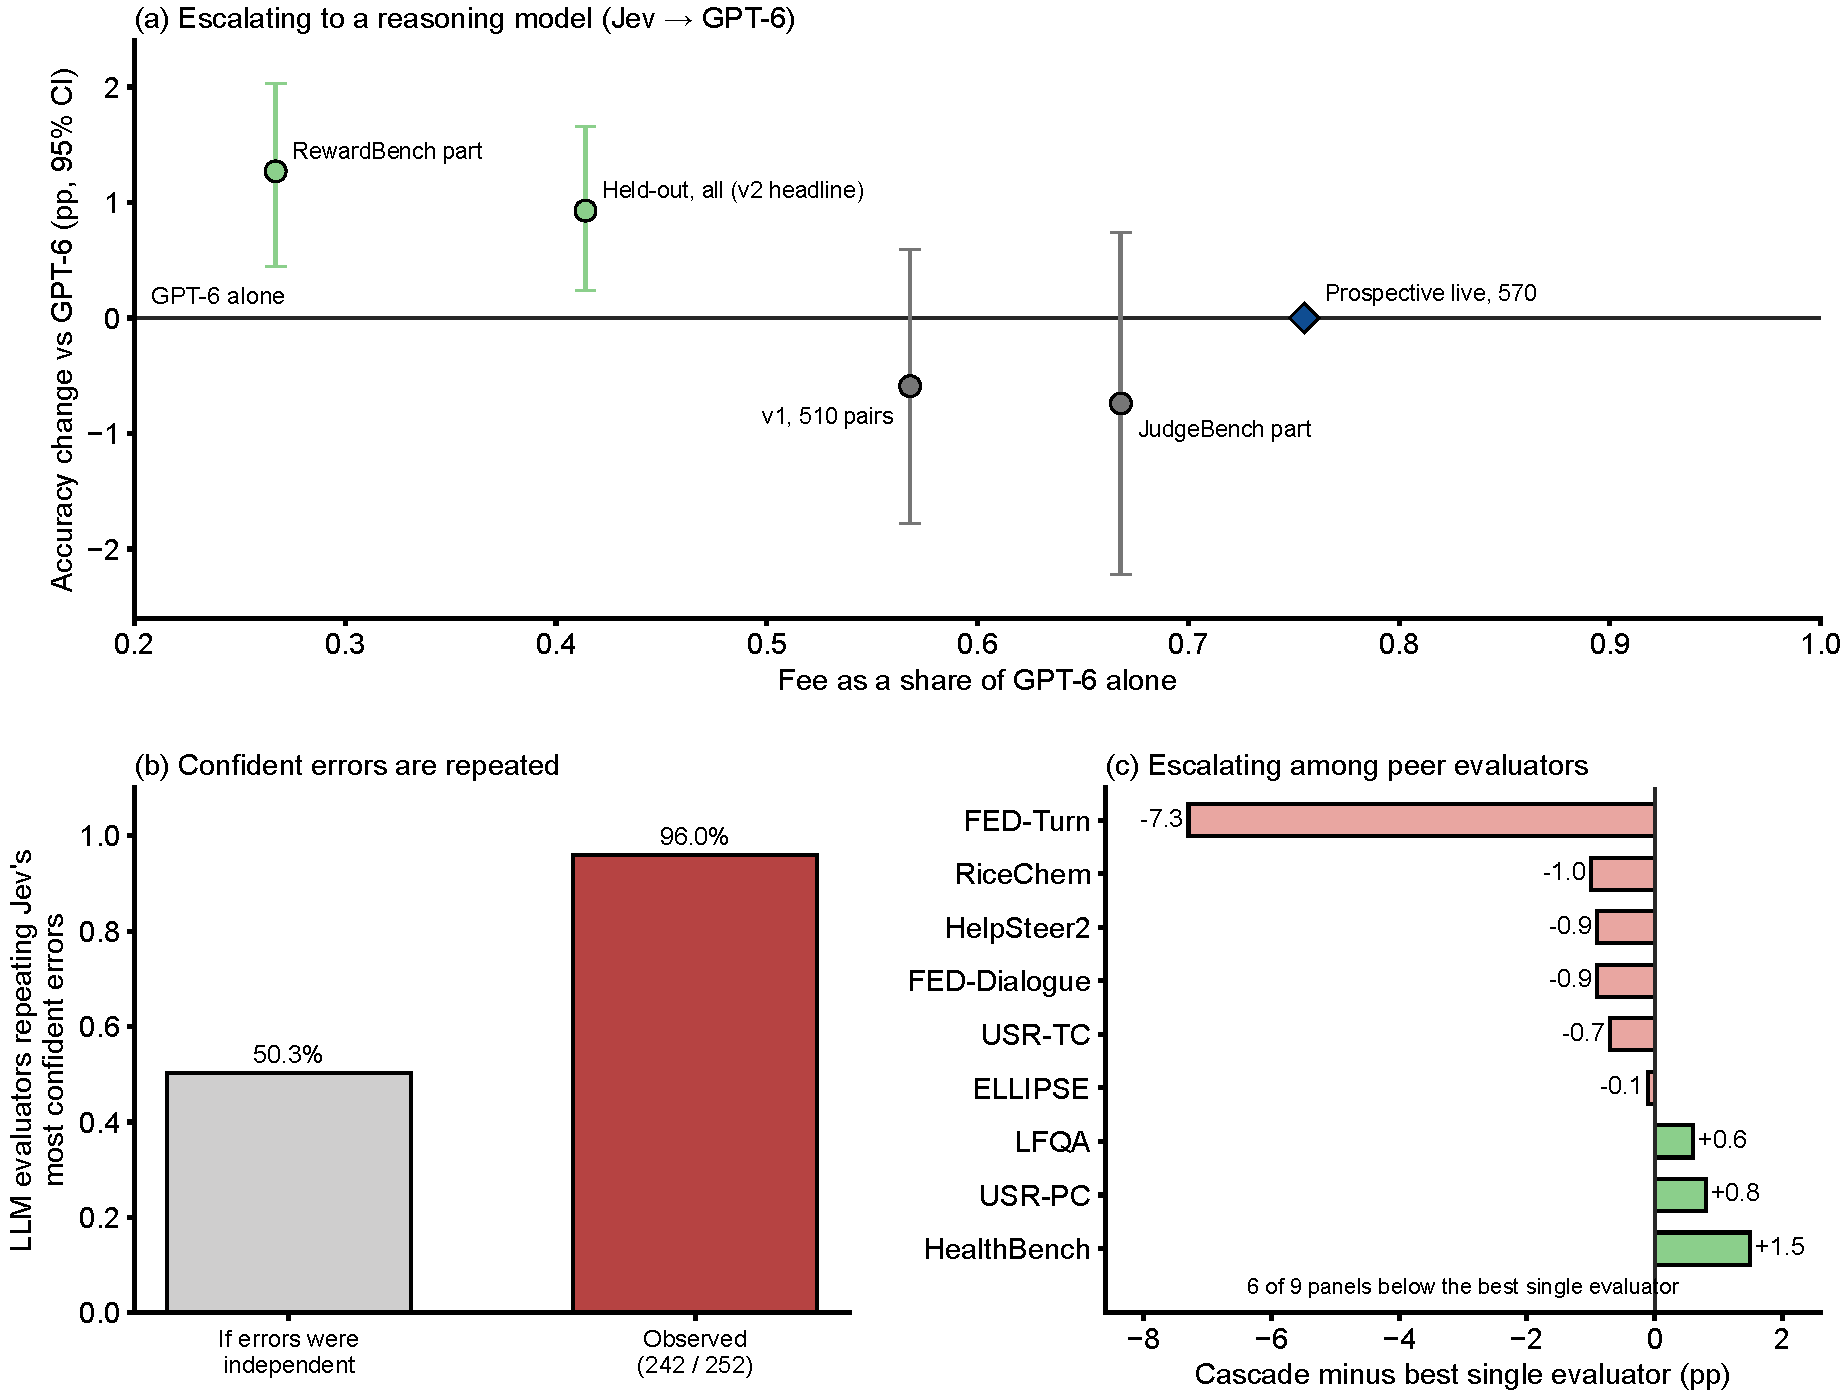
\includegraphics[width=0.9\linewidth]{figures/fig_escalation.pdf}
\caption{G6：升级。
(a) 从 \jev{} 到 GPT-6 的“有把握即接受”级联：准确率变化与费用占比~\protect\cite{arx26550}；灰色点的区间包含零，菱形为前瞻性实时测试。
(b) \jev{} 置信度最高的错误被低成本生成式评估器重复的比例，与错误相互独立时的预期比例对照~\protect\cite{arx29769}。
(c) 全部九个面板上交叉拟合级联减去最佳单一评估器的差值~\protect\cite{arx29769}。}
\label{fig:escalation}
\end{figure}

% ---------------------------------------------------------------------------
\subsection{G7——公共规模的判断与模拟}
\label{sec:g7}

\begin{answerbox}
类型化模型使人口规模的阅读与模拟变得廉价，部分研究展示了如何诚实地做到这一点：抽样审计，并将测得的与真实人群之间的差距带入每一项结论。
模拟公众偏向某一人群并低估分歧，且部署依赖于单一闭源厂商。
编码：S~5，Q~12，N~2。
\end{answerbox}

KITE~\cite{arx27535} 对每个唯一状态调用 \jev{} 一次，通过查表在一秒内模拟一百万个智能体，并将测得的人类--模型差异作为共享误差项传递至每一项结论；在 37 项未见研究上，该误差项在名义 80\% 和 90\% 水平下给出的回溯覆盖率分别为 0.93 和 0.96，高于名义水平，可能偏保守，但其预注册的主要终点未显示明显增益。
一项全州范围的研究用 \jev{} 阅读了约五十万份警方叙述，通过盲法人工裁定审计了一个按概率分层的样本，并报告了带区间的、经误分类校正的计数，同时发现在两轮脱敏后，记录胎儿伤害的叙述中有 43\%、裁定样本中有 37\% 仍残留个人标识信息~\cite{arx00213}。
在无人设时，\jev{} 回答价值观问题的方式与其美国人设相似，并在标注者意见分歧之处保持高置信（\cref{sec:g3,sec:g4}），因此模拟公众偏向某一人群并低估分歧~\cite{arx36399,zen23032384}\zmark{}。
匹配基准显示，托管 \jev{} 每千次决策成本不足一美分，中位延迟为 138\,ms~\cite{arx00346}；其权重未公开，也不提供自托管，这促使一项路由研究将其接口设计为与分类器无关，并配备自托管的后备方案~\cite{arx28919}。
一篇概念性论文认为，更廉价的评估可能增加而非减少评估总量和异常处理~\cite{arx01231}。
此处的诚实性条件即调查方法论和关注分歧的标注~\cite{davani2022dealing,plank2022problem}所要求的条件。

% ---------------------------------------------------------------------------
\subsection{跨要求综合}
\label{sec:across}

在 \nRows{} 个已编码的研究--要求配对中，\nS{} 个支持检测器用途，\nQ{} 个为有条件（Q），\nN{} 个为不支持（N）（\cref{fig:framework}）。
仅保留较强设计的研究时（\nStrongRows{} 个中 \nStrongS{}、\nStrongQ{} 和 \nStrongN{} 个），或剔除 Zenodo 记录时（Zenodo 记录被编码为 N 的比例高于 arXiv 论文：44 个配对中 19 个，对 107 个中 25 个；剔除后为 \nNoZenRows{} 个中 \nNoZenS{}、\nNoZenQ{} 和 \nNoZenN{} 个），各比例变化约六个百分点或更少。
七十六个配对在同一要求上将类型化模型与生成式评估器进行了比较：类型化模型在 23 个中更好，17 个中相近，28 个中不一，8 个中更差。
具体就失效而言，图景更为单薄且更不利：在有对照的 14 个 N 编码中，类型化模型在 6 个中更差，4 个中相近，3 个中不一，1 个中更好；而 48 个 N 编码中有 34 个完全没有对照。
因此，证据既未表明类型化模型总体上差于生成式评估器，也未表明其失效与后者共有；对多数失效而言，这一比较尚未进行。
有两种失效模式源于类型化接口本身：所报告的置信度可能因填充选项集而被抬高（G4），且决策不附带理由（G5）；第三种，即概率向量为攻击者提供指引，仅在一项研究中得到证明（G2）。

综合来看，这些编码仅在全文所用的限定意义上支持检测器用途：几乎每一项成功都依赖于某一附加条件，如本地拟合的阈值、第二道独立核查或人工审查；而 G2 和 G4 中的失效是检测器本身的失效，因为被操纵或沉默的检测器会漏掉违规。因此，\cref{sec:design} 的建议并非认为类型化检测器可靠，而是认为：在检测器角色中（每一项具有实质后果的动作都须经过另一道核查），其失效比在裁决者角色中（没有任何此类核查）更易于以较低代价加以控制。

\Cref{tab:keyfindings} 列出了被纳入\cref{sec:synthesis,sec:design}及摘要的发现，并给出各自的确定性：按\cref{sec:appraisal}的规则评定，纳入主窗口和更新检索中与该发现相关的全部已编码研究；为便于比较，同时列出 10 月 4 日给定的评级。没有任何发现达到中等确定性，有四项发现有争议。

\begin{table}[!htbp]
\centering
\footnotesize
\setlength{\tabcolsep}{3pt}
\caption{主要发现及证据确定性。\emph{范围}：托管 \jev{}、开源模型或两者（泛指类型化模型）；关于托管 \jev{} 或两者的发现仅依据托管模型证据评级，按系统组计数。\emph{编码}：支持研究的编码。\emph{来源}：先列主要支持研究，再列相反研究（计入的每项研究及其方向均列于 \nolinkurl{data/certainty_evidence.csv}）；“更新：”为更新检索研究；“开源：”为开源模型研究，起佐证作用（标为“开源，反向：”者则指向相反方向），但不计入评级。确定性的定义见\cref{sec:appraisal}；$^{c}$~在该范围内有争议；$^{j}$~依判断评级的描述性计数。\emph{10 月 4 日}：10 月 4 日给定的评级（所引研究，旧规则）；$^{a}$~按现行规则为极低（\cref{sec:certainty-detail}）。\emph{当前}：现行规则，纳入全部已编码的主窗口与更新研究（仅主窗口：\cref{tab:certchanges}）。由 \nolinkurl{scripts/rate_certainty.py} 根据 \nolinkurl{data/certainty_evidence.csv} 计算。}
\label{tab:keyfindings}
\begin{tabularx}{\linewidth}{@{}L>{\raggedright\arraybackslash}p{0.06\linewidth}>{\raggedright\arraybackslash}p{0.055\linewidth}>{\raggedright\arraybackslash}p{0.12\linewidth}>{\raggedright\arraybackslash}p{0.17\linewidth}>{\raggedright\arraybackslash}p{0.08\linewidth}>{\raggedright\arraybackslash}p{0.08\linewidth}@{}}
\toprule
发现 & 范围 & 编码 & 与生成式比较 & 来源 & 10 月 4 日 & 当前 \\
\midrule
零样本下对有害或未对齐内容排序良好，成本仅为一小部分；常不及最佳 LLM 准确 & 托管 & S/Q/N & 更好（低成本）；更差（最佳） & \cite{arx29429,jkf87_2026replication,zen22885291,arx33401,arx24574,arx27678} & 低 & 低 \\
固定阈值不可迁移；需本地拟合 & 两者 & Q & -- & \cite{arx29429,jkf87_2026replication,arx00346,arx01006,arx26550,arx24574,arx02046}；相反：\cite{arx33689}；更新：\cite{arx03387,arx02267,zen22935043} & 低 & 低$^{c}$ \\
错误集中于被总体指标掩盖的子类型 & 托管 & Q & 不一 & \cite{arx33401,alphaRAG,arx02046}；更新：\cite{arx07953,arx03324,arx08675,arx10321} & 极低 & 低 \\
插入的观点、经优化的上下文和词汇诱饵可操纵决策 & 两者 & N & 相近 & \cite{arx31142,arx01834,arx01006,arx30243,arx02048}；开源：\cite{zen22959854,zen23038928} & 低 & 低 \\
指令注入很少选中攻击者的目标（原始 1.8\%，自适应 3.5\%） & 托管 & S & -- & \cite{arx28613}；相反：\cite{arx31142,checkpoint2026jev}；更新，相反：\cite{arx04985} & 极低 & 极低$^{c}$ \\
选项名称可能压过定义；中性标识符可消除其大部分 & 两者 & N & -- & \cite{arx26758,arx00346}；更新：\cite{arx07953}；开源：\cite{arx02586} & 低 & 低 \\
默认偏向某一种文化的价值观 & 托管 & N & -- & \cite{arx36399} & 极低 & 极低 \\
在熟悉的封闭选择任务上校准良好，与前沿模型相比结果不一；校准是局部的 & 托管 & S/Q & 更好或不一 & \cite{arx37647,arx01006,arx24052,arx27607,arx24574,arx34024,zen22885291} & 低 & 低 \\
显式“不知道”在正确时很少被选中；“以上皆非”的选择不一致 & 托管 & Q/N & 相近或更差（前沿）；更差（推理） & \cite{arx34024,arx39496,arx01006}；更新：\cite{arx03387,arx06425} & 低 & 低 \\
另设的充分性问题可检测信息缺失，但筛选答案的效果不如置信度 & 托管 & Q & -- & \cite{arx01006} & 极低 & 极低 \\
升级至更强的推理模型可在可读出的判断上节省成本且准确性无损失 & 两者 & Q & 相近 & \cite{arx26550,arx24574,arx02046}；开源：\cite{zen22922769}；更新，相反：\cite{arx02267}；开源，反向：\cite{arx07177,arx03324} & 低 & 低$^{c}$ \\
以与独立构建规则一致为接受条件，macro-F1 无损失，但被标记的伪装攻击更少 & 两者 & Q/N & 相近 & \cite{arx02048}；更新，开源：\cite{zen22904595} & 极低 & 极低 \\
同类评估器重复 \jev{} 置信度最高的错误（上界） & 托管 & N & 相近或不一 & \cite{arx29769,arx33401} & 低 & 低 \\
预先设定的阈值在新数据上未达到错误目标 & 两者 & Q/N & -- & \cite{arx33401,arx24574}；相反：\cite{arx33689}；开源：\cite{arx33843,zen23041163,arx07177}；更新：\cite{arx03387,arx02267}；更新，相反：\cite{zen22935043,zen23075657} & 中等$^{a}$ & 低$^{c}$ \\
类型化模型总体上并不差于生成式评估器；多数失效缺乏对照比较 & 两者 & -- & 76 个中 23 个更好、8 个更差 & \cref{app:evidence} & 低 & 低$^{j}$ \\
尚无研究测量 \pol{} 构念（三值、中文） & -- & -- & -- & -- & -- & -- \\
\bottomrule
\end{tabularx}
\end{table}

\FloatBarrier

% ---------------------------------------------------------------------------
\subsection{更新检索（2026 年 10 月 2--8 日）}
\label{sec:update}

更新检索（\cref{sec:search}）新增 \nUCoded{} 个已编码来源：\nUSetPostWindow{} 个于 10 月 2--8 日首次发布，\nUSetLateIndexed{} 篇为迟索引的 arXiv 论文，\nUSetReScreened{} 条为重新筛选的 Zenodo 记录。
其 \nURows{} 个研究--要求配对的编码为 S~\nUS{}、Q~\nUQ{}、N~\nUN{}（仅较强设计研究：\nUStrongRows{} 个中 \nUStrongS{}、\nUStrongQ{} 和 \nUStrongN{} 个）；这些配对未合并入上文的计数，\cref{tab:update} 将其与主窗口并列。
作为敏感性检验，我们将日期在主窗口之内的 18 条记录（36 个配对：S~5，Q~28，N~3）加入主计数；这不改变任何简要回答，最常见的编码仅在主窗口中 Q 与 N 几乎持平之处发生变化（G3：N~12 对 Q~10 变为 Q~14 对 N~13；G5：3--3 持平变为 Q~4 对 N~3）。
该检验仅涉及编码的方向；它不重新计算对照比较的比例，而\cref{tab:keyfindings} 中的确定性评级是在加入全部更新研究（包括这 18 项）后评定的。
更新集合中 N 编码的比例低于主窗口（配对的 12\% 对 30\%）：仅有一项新研究攻击了类型化模型（G2，即编码最为不支持的要求），且多数新配对的结果不一。
在其 14 个 N 编码中，9 个有生成式对照，其中类型化模型在 6 个中更差，这 6 个中有 4 个仅涉及开源模型；两个集合合计，62 个 N 编码中仍有 39 个缺乏对照。

没有任何简要回答被推翻。
新证据限定了一项表述，即 G5 中关于分解链路的表述，该简要回答已相应修订；其他简要回答不变，新证据大多对其予以确认。
\cref{sec:appraisal} 的确定性规则在评审期间（这些研究完成编码之后）进行了修订，每项发现均依据全部已编码的主窗口和更新研究按该规则重新评级；这构成一项方案偏离，因为更新方案原已冻结主窗口的评级。
与仅依据主窗口研究相比，更新研究改变了一项评级：两项关于托管 \jev{} 的较强设计研究将“预先设定的阈值在新数据上未达到错误目标”这一发现从极低提升至低，但仍有争议~\cite{arx03387,arx02267}，另有两项研究的阈值达到了目标，增加了相反证据~\cite{zen22935043,zen23075657}\zmark{}。更新研究还使“升级至更强的推理模型”这一发现有争议，因为一项 \jev{} 预筛仅使一个安全审核者的成本降低 4.3\%~\cite{arx02267}；并为注入发现（主窗口中已有争议）增加了一项相反研究。
各项发现的推导过程及相对 10 月 4 日的变化见\cref{sec:certainty-detail}。
下文按要求逐项给出与 \pol{} 最直接相关的研究。

\begin{table}[!htbp]
\centering
\footnotesize
\caption{主窗口与更新检索中按要求划分的编码（S/Q/N）。\emph{更新}：全部更新配对；\emph{窗口内}：来自 \nUSetLateIndexed{} 篇迟索引 arXiv 论文和 \nUSetReScreened{} 条重新筛选 Zenodo 记录、日期在主窗口之内的配对；\emph{主窗口 + 窗口内}为敏感性检验。最后一列：有生成式（生成）对照的更新配对中，类型化模型更好、相近、不一或更差的数量，以及无对照的配对数。数据：\nolinkurl{data/evidence_coding_update_2026-10-08.csv}。}
\label{tab:update}
\begin{tabular}{@{}lccccc@{}}
\toprule
要求 & 主窗口 & 更新 & 窗口内 & 主窗口 + 窗口内 & 更新与生成式比较；无 \\
\midrule
G1 & 2/20/5 & 2/17/3 & 1/9/0 & 3/29/5 & 1/4/7/3；7 \\
G2 & 1/0/9 & 0/0/1 & 0/0/0 & 1/0/9 & --；1 \\
G3 & 2/10/12 & 5/15/3 & 1/4/1 & 3/14/13 & 3/2/3/0；15 \\
G4 & 3/29/13 & 3/26/3 & 2/6/1 & 5/35/14 & 6/0/7/3；16 \\
G5 & 2/3/3 & 0/6/0 & 0/1/0 & 2/4/3 & 1/1/2/0；2 \\
G6 & 1/23/4 & 1/19/3 & 1/7/1 & 2/30/5 & 3/3/2/0；15 \\
G7 & 5/12/2 & 1/9/1 & 0/1/0 & 5/13/2 & 1/0/6/1；3 \\
\midrule
全部 & \nS{}/\nQ{}/\nN{} & \nUS{}/\nUQ{}/\nUN{} & 5/28/3 & 21/125/51 & 15/10/27/7；59 \\
较强设计 & \nStrongS{}/\nStrongQ{}/\nStrongN{} & \nUStrongS{}/\nUStrongQ{}/\nUStrongN{} & -- & -- & -- \\
\bottomrule
\end{tabular}
\end{table}

\paragraph{G1：得到确认。}
三项新研究检验了仇恨言论与内容审核，即安全阀的核心。
在未经任务训练的情况下，\jev{} 在四个英文数据集上的二分类仇恨言论 macro-F1 分别为 0.826、0.691、0.738 和 0.960，而 GPT-6 Sol 为 0.897、0.682、0.776 和 0.976；商用 LLM 仅在一个数据集上显著领先于每一个决策模型；所有模型（类型化与生成式）均难以区分仇恨言论与仅具冒犯性的语言（三分类：\jev{} 0.532，Sol 0.604，一个监督式 TF-IDF 分类器 0.639）~\cite{arx03324}。
这比“常低于最佳评估器”所暗示的更接近最佳 LLM，但仍在简要回答所述方向之内。
在在线内容审核中，\jev{} 在两个英文数据集上的 F1 与 Detoxify 持平或更高（但其在其中一个数据集上的准确率较低，74.4\% 对 81.0\%），在一个 Bluesky 基准上的 AUROC 为 0.89--0.90；但其在 Facebook 仇恨言论政策选择上的精确匹配准确率在无检索先例时为 29.4\%（有先例时为 51.6\%），在一个社区规则测试集上的得分低于始终回答“no rule broken”（未违反任何规则）（48.4\% 对 50.0\%）~\cite{arx07953}。
在 ToxicChat 上，基于 1{,}000 个开发标签选定的阈值，在一个由先前已观测条目构成、带混合标签的测试集上，以 3.24\% 的误报率取得 90.52\% 的召回率，处于该研究 5\% 的容差之内，而三种固定编码器条件的召回率为 35.6--58.9\%；在一项事后细分中，仅就人工标注的负例而言，误报率为 5.39\%~\cite{zen23075657}\zmark{}。
作为提示注入、越狱、有害内容和 AI 生成文本的零样本检测器，托管 \jev{} 在八个基准上的 AUROC 为 0.95--1.0，但其准确率（在六个安全基准上为 87--99\%）是在基于留出样例拟合的阈值下测得的；在 AI 生成文本上，准确率仅在采用此类阈值时才从默认阈值下的 78\% 升至 89\%~\cite{arx04985}；在一个智能体测试框架中，它对注入的筛查效果良好（AUROC 0.98），却放过了 25.5\% 的有害请求，且无法用作个人数据门控（误报率 63--66\%）~\cite{arx02267}。
在 AgentHarm 的有害性判断上，在单次运行中它与九种生成式配置中的最佳者持平（84.54\% 对至多 85.57\%）~\cite{arx03935}。
总体指标再次掩盖了子类型失效：在已编码字段同时记录了该因素的情形下，人工编码者确认了 \jev{} 交通事故叙述标记的 96--100\%，但对未系安全带的乘员为 15\%~\cite{arx10321}；该研究是对~\cite{arx24052}的扩展，出自同一作者并使用复用数据，因而与之并不独立。
两个开源类型化模型在相同基准上的得分低于生成式对照~\cite{arx06744,arx07177}；在工业故障检测中，托管 \jev{} 标记了 57--94\% 的无故障窗口，并且在九项偏移测试下，其表现并不优于标记每一个窗口~\cite{arx09937}。

\paragraph{情绪与中文文本（T1）。}
在八个情感基准上进行零样本测试，\jev{} 的平均 macro-F1 为 62.93\%，高于十种生成式配置中的五种，低于最佳者（67.28\%），成本比最佳者低 96\%；在中文情绪分类（CMMA）上，所有系统表现均弱（\jev{} 21.06，生成式模型 19.82--23.31）~\cite{arx08829}。
这项单次运行研究分类的是文本所表达的情绪，而非人的状态，因此它涉及的是 T1 会保留的边界一侧（\cref{sec:synthesis}）：如今为每条消息给出情绪分数已很廉价，而在中文文本上这些分数并不准确。
没有新研究在中文上操纵语言；一项基于中文请求构建的工程基准在 G4 下讨论~\cite{arx09896}。

\paragraph{G2：得到确认。}
一项新研究攻击了托管 \jev{}：一种针对 \jev{} 的注入和一个通用后缀在三项任务上达到 97--100\% 的攻击成功率，且投毒 5--10\% 的训练数据即在一个开源模型中植入了后门~\cite{arx04985}。
这一攻击的成功率远高于主窗口中那项支持研究中的攻击（1.8\% 的目标选中率）~\cite{arx28613}，后者使用的是不同的攻击和基准；该发现此前已因针对托管 \jev{} 的其他攻击而有争议~\cite{arx31142,checkpoint2026jev}，其确定性仍为极低。

\paragraph{G3：得到确认。}
为每个仇恨言论数据集提供其自身的定义，改变了决策模型 2.8--27.9\% 的预测，显著提升与显著下降同样频繁（28 次比较中各 8 次）；\jev{} 最不敏感，而一个经政策训练的生成式模型在四个数据集中的三个上一致性也有所下降~\cite{arx03324}。
将不透明的政策标识符替换为可读的仇恨言论政策名称，使 \jev{} 的二分类准确率下降 5.06 个百分点（CI 3.91--6.21）~\cite{arx07953}；在三个开源 Laya 检查点中，与其定义相矛盾的标签使准确率降至 0.14，低于无信息对照~\cite{arx02586}。
然而，中性标识符并非没有代价：在匹配对照中，它们使一个开源生成式读出对缺失答案的检测下降 20--31 个百分点~\cite{arx03387}。
选项顺序对托管 \jev{} 的影响远小于对开源类型化模型的影响（决策变化率 1.8\%，Laya 为 30.3\%~\cite{arx02267}；顺序敏感性 0.039，Laya 各变体为 0.37--0.59~\cite{arx02293}），且 \jev{} 的顺序一致性高于 Qwen3-32B~\cite{arx09188}，与“稳健性因模型而异”一致；但改写定义或以不同方式呈现相同证据仍会改变其答案~\cite{arx09937,arx08675}，且顺序翻转集中于其不确定之处~\cite{arx06625}。
一个基于挪威和奥地利登记册文本训练的开源模型，在奥地利测试集中 94.6\% 的规则类型上与参考一致，而在一个未见过的丹麦登记册上为 62.4\%~\cite{zen23225893}\zmark{}。

\paragraph{G4：得到确认。}
与前沿模型的比较结果仍然不一。
在一个包含 10{,}938 个问题的双语基准上，\jev{} 的 ECE 低于所有生成式配置（0.053 对 0.078--0.253），但它将 89\% 的概率质量置于众数上，而真实比例为 36\%~\cite{arx03935}；在八项人工标注的阅读任务上，它的校准优于一个前沿模型的词元概率，但在成对任务上，一个 27B 开源模型校准更好~\cite{arx06625}；在中文工程问题上，其 ECE 为 0.027，而三个旗舰 LLM 的自述概率为 0.031--0.061，尽管它在 5{,}000 条记录中有 678 条失败~\cite{arx09896}；在其自身生成的博弈状态中，它差于常数预测器（Brier 0.283 对 0.250），而一个通过选项概率读出的小型生成式模型胜过该常数预测器~\cite{zen23221456}\zmark{}。
在冒犯性语言和仇恨言论任务上，无检索先例时其概率校准不佳（OLID 上 ECE 14.9\%，HateXplain 上 33.2\%；有先例时为 9.7\% 和 20.2\%）~\cite{arx07953}。
在弃权方面，设有显式 NONE 选项时，\jev{} 在正确答案被人为移除的条目中拒绝了 63.7\%，错误拒绝率为 3.3\%（一个开源生成式读出：45.0\%），在第二项任务上为 82.4\%，但随着候选项增加，检测率下降~\cite{arx03387}；未针对该任务训练的托管 \jev{} 对 382 个不可回答条目中的 62.8\% 给出了确定答案，而作者的循环（looped）模型为 17.5\%~\cite{arx07730}；在一个开源 \jev{} 式读出中，显式 ABSTAIN 选项拒绝了 30 个无有效答案案例中的 28 个，但在 30 个有效案例中仅 17 个选择正确~\cite{arx07327}。
在提供拒绝或升级选项时，托管 \jev{} 在 48 份无有效候选的合同中有 45 份请求新候选，但在 120 个无可行路径的转发实例中仅升级了 4 个~\cite{arx06425}。
这些结果与简要回答相符：显式的“不足”选项仅部分有效，且“以上皆非”（none）的选择不一致——在关于托管 \jev{} 的各项研究中，对无答案条目的选择比例为 3--94\%~\cite{arx39496,arx03387,arx06425}。

\paragraph{G5：一项表述受到限定。}
两项研究将一个判断分解为若干标准问题并以固定规则组合：在仇恨言论上，这在 30 次比较中有 6 次提高、11 次降低了 macro-F1，且 \jev{} 的唯一一次提升可由调优后的阈值同样达到~\cite{arx03324}；在八个情感基准上，它使 \jev{} 的平均值从 62.93\% 降至 57.31\%，而将这些判断附加到状态中也未更准确（61.61\%）~\cite{arx08829}。
在另外两项研究中，仅暴露与当前步骤相关的字段，或将核查移入一个单独的门控，提高了正确决策数（120 个中从 90 增至 113；120 个中从 29 增至 84）~\cite{arx07327,arx06425}。
因此，分解可使链路可检查，但仅在部分情境下提高准确性，G5 的简要回答现已如此表述。
一个概念验证记录并重构了两个实时决策，但仅在其作者构建的确定性外壳之内，且输出不附带理由~\cite{zen23189584}\zmark{}，这确认了“可以被记录，但无法被解释”。

\paragraph{G6：得到确认，但一致性较低。}
预先固定的阈值在新数据上常常未达到其目标，但并非总是如此：在一项任务上校准的拒绝阈值，在 12 次迁移中有 6 次超过了 5\% 的错误拒绝目标~\cite{arx03387}；分裂共形预测达到了其边际目标，尽管在该方法下 \jev{} 的单标签答案在名义 5\% 水平下有 5.93\% 是错误的~\cite{zen22935043}\zmark{}；基于训练登记册拟合的弃权阈值在奥地利测试集上守住了预注册的 2\% 目标（1.3\%），但在一个未见过的登记册上产生了 14.3\% 的风险，而目标为 5\%~\cite{zen23225893}\zmark{}。
认证也可能拒绝给出：在同一研究中，一种界限为近似界限而非精确有限样本界限的程序，在 2{,}000 次划分中的任何一次上都无法为 \jev{} 在 AG News 上认证 5\% 的自动层级（在 SST-2 上为 2{,}000 次中的 191 次）；一种探索性的替代阈值规则在 2{,}000 次 SST-2 划分中认证了 1{,}776 次，但在 AG News 上仅 4 次~\cite{zen22935043}\zmark{}。
在内容审核中，仅接受置信度 $\geq 0.8$ 的 \jev{} 决策覆盖了一个 Bluesky 基准的 71.9\%，准确率为 94.3\%，但在仇恨言论政策选择上，被接受决策的准确率仅为 75.8\%，在社区规则上为 67.6\%~\cite{arx07953}。
升级至更强的推理模型在部分研究中有所帮助：以推理模型 30\% 的调用次数达到与之相当的水平~\cite{arx09683}；在一项探索性分析中，由前沿模型（GPT-6 Sol）复核 Laya 最不确定的五分之一条目提高了仇恨言论 macro-F1，但在三个数据集中的两个上未达到该前沿模型自身的水平，而转交一个更廉价的模型（GPT-5.6 Luna）则在一个数据集上使其下降~\cite{arx03324}；但在另一些研究中并无帮助：一个从接近随机水平的开源类型化评估器出发的预注册级联几乎将每个条目都升级~\cite{arx07177}，而在计入其自身词元后，\jev{} 预筛仅使一个 LLM 安全审核者的成本降低 4.3\%~\cite{arx02267}。
将 \jev{} 最不确定的重排序标签升级至 Qwen3-32B 从未带来帮助~\cite{arx09188}；在该任务上，Qwen3-32B 的准确性与 \jev{} 大致相当（与人工评分者的一致率 87.2\% 对 86.2\%，但重排序器 NDCG@10 略低，0.630 对 0.637），因此计为同类模型（\cref{sec:appraisal}），该结果正是简要回答对同类模型所预期的。
在由独立构建的核查掌握决定权之处，依据类型化决策采取行动是安全的~\cite{arx07327}；一个预先固定且带有基于规则后备方案的门控在新数据上保持有效~\cite{zen23088660}\zmark{}。
简要回答仍然成立，但关于升级可节省成本且准确性无损失的证据不如主窗口中一致：其确定性仍为低，且该发现现已有争议（\cref{tab:keyfindings}）。

\paragraph{G7：得到确认，并新增一项关于隐私的不支持证据。}
在 HateCheck 上，\jev{} 每 1{,}000 条文本的成本为 0.033 美元，中位延迟 336\,ms，而 GPT-6 Sol 为 1.177 美元和 1{,}426\,ms，\jev{} 的 macro-F1 比后者低 1.6 个百分点~\cite{arx03324}；但在七项政治学任务中的六项上，按批量价格计算，它并不比前沿模型便宜~\cite{arx06625}。
对 229{,}510 份交通事故叙述的两层概率抽样给出了经盲法人工层确认的全州计数，但这仅在逐因素的人工重新校准之后才实现~\cite{arx10321}，即简要回答所描述的设计。
作为群体投票分布的替代，\jev{} 的 Choice 概率在人们以 55 比 45 分歧的安全条目上报告了 0.88，表现差于均匀猜测~\cite{zen23179064}\zmark{}，这确认了它会低估分歧。
新的是关于隐私与双重用途的证据：用户输入中的条件指令使托管 \jev{} 仅凭其标签即在每个受测案例中泄露了隐藏的性别、年龄组、心脏病和族裔属性；\jev{} 被用作判定接口（oracle），提高了有害计划被评判的有害性；其 200 个标签将一个替身模型的一致率从 49\% 训练至 92\%~\cite{arx04985}。
这将不向不受信任的调用方提供概率的理由（\cref{sec:design}）扩展至放入检测器输入中的字段，以及不受信任的调用方可查询的任务。

\section{规范中的五处张力}
\label{sec:synthesis}

对照证据阅读，该规范在五处向两个方向拉扯，而低成本的类型化判断使其中每一处都从一个哲学问题变成一项工程默认设置。
对每一处张力，我们给出对文本最善意的解读、与之相关的证据以及若干选项，其中至少有一个选项保留原文不变。
在各选项之间作出选择，属于该框架的作者以及将来实施它的人。

\paragraph{T1. 理解语言中的情感与检测个人的情感状态。}
\Clause{4.3} 指出，“毫无必要让 PAI 检测一个人的情感状态”，因为情感状态是转瞬即逝的、个性化的、情境敏感的，并涉及人的尊严；\clause{4.3.3.1} 要求 PAI “理解人类情绪状态和过程”；\clause{4.3.3.3} 则以两个关于小狗狗的问句说明语义识别，二者的区别在于话语的意图。
将这些条款合读，可以得到一种一致的解释：识别话语的情感意义与意图，但绝不推断个人的内心状态。
然而，文本并未明示这一边界，而类型化模型使得为每条消息附加情绪分数几乎毫无成本，这正是该边界在实践中被越过的方式。
关于情感相关判断的证据薄弱且结果不一：在一项标注研究中，\jev{} 对大多数共情条目给出了高置信度，但在其置信度最高的条目上，准确率几乎不高于全部条目（0.383 对 0.371，三类均衡），作者在一个低成本生成式模型中也发现了同样的失效~\cite{arx24574}；而在多语言效价--唤醒度回归任务上，加装了一个针对标签拟合的监督层的 \jev{} 与最佳系统持平~\cite{arx35293}。
更广泛的文献则更为明确：从可观察信号推断情绪在科学上依据薄弱~\cite{barrett2019emotional}，在伦理上问题重重~\cite{stark2021ethics}。
\emph{选项：}明确写出这一边界，使保障机制判断话语的语义与意图，但绝不为个人赋予情感状态；并将情感相关判断保留给 PAI 审计其\emph{自身}输出之用，例如审计 \clause{4.3.2} 所称构成情感操控的虚假亲密关系。

\paragraph{T2. 二值判定与三值伦理。}
\pol{} 建立在爱/恨两极之上，但增设了不在场状态（\clause{4.3.2}），并告诫其概念服务于结构性分析而非道德标签（\clause{1.5}）。
“这是恨语吗？”这样的是/否问题把这两项限定都舍弃了。
证据从多个方向指向同一结论：选项名称可以左右判定结果~\cite{arx26758,arx00346}；在模型不确定之处，互补概率之和不等于一~\cite{arx33209}；显式的“不知道”选项在其为正确答案时很少被选中，“以上皆非”也只是不稳定地被选中（在一个医学基准上为 54\%，在识别它需要算术推理时为 7\%）~\cite{arx34024,arx39496}；是/否概率把冲突与无知置于同一区间，而一个分别列出这两种状态的 Choice 问题在四个案例中把二者区分开来~\cite{zen22848952}\zmark{}。
证据也表明了什么有帮助：单独询问证据是否充分的是/否问题，在发现信息缺失方面优于置信度，尽管它作为接受答案的筛选器较弱~\cite{arx01006}。
\emph{选项：}将每个爱/恨问题都设为三值，把不在场或信息不足列为显式选项，并将充分性作为单独的问题提出、监测其使用率；将“有争议”（人们意见分歧）作为一个单独的标记交由人处理，与“不在场”相区分；并通过把中性标识符绑定到定义、再以重命名加以检验的方式，使道德词汇不出现在选项名称中。
这些选项是在实施 \clause{1.5} 与 \clause{4.3.2}，而非改变它们。

\paragraph{T3. 完全透明与封闭模型。}
\Art{4} 与 \art{5}(4) 要求运行逻辑和决策过程“完全公开透明”，并要求技术“不应是黑箱”。
TypeSafe 既未公开托管版 \jev{} 的权重、架构、奖励，也未公开其训练数据，且不提供自托管~\cite{arx24574,arx28919,arx00346}。
一种善意的解读是，\art{4} 关注的是 NaturalDAO 的流程与资源流向的透明，而记录一个封闭组件的输入、输出、版本与校准数据可以部分满足这一要求；但此类日志无法显示该组件如何得出其输出，而仅凭开放权重也无法提供 \art{5}(5) 所要求的“推理步骤”。
开源模型使读出过程可被检查，但在若干比较中其准确性或鲁棒性较差：Laya 表现出最严重的名称反转，在交互风险筛查上接近随机水平~\cite{arx26758,arx33401}。
这一差距并非固定不变：更大的开源解码器在选项名称互换下比 \jev{} 更鲁棒~\cite{arx00346}；由 Laya 初始化的中文模型在其作者的通用基准上、以及经领域微调后在医学领域略微超过 \jev{}，尽管在各专业领域上的平均准确率为 \jev{} 的 92\%~\cite{arx36965}；而且已有一套开放的 RLCD 方案~\cite{arx38850}。
\emph{选项：}（a）仅将封闭模型用作外部基线，而在可自托管的模型上运行具有实质后果的判断，并在每条决策记录中固定其权重、版本与校准数据；或（b）允许封闭模型作为若干独立检测器之一，同时记录其输入、输出与版本。
选项（a）以已测得的准确性与鲁棒性换取可检查性；这一权衡应明确作出，并随开源模型的进步而重新审视。
公开决策记录还与不向攻击者泄露概率相冲突（见\cref{sec:g2}），\cref{sec:design} 通过延迟并粗化公开内容来化解这一冲突。

\paragraph{T4. 纯 AI 裁决与相关错误。}
\Art{2}(1) 规定 NaturalDAO “在与全人类密切协作的前提下”自主完成决策，\art{10} 将争议交由 AI 进行事实分析与伦理评估，并接受人类质询，\art{9}(7) 则规定人类监督“不直接干预”决策，质询中提出的问题由 NaturalDAO 自主处理。
文本并未说明协作这一前提如何约束具体决策。
证据从两方面涉及非干预原则。
升级可能保留错误：在基于评分细则的评分任务上，低成本生成式评估器在 96\% 的情形中重复了 \jev{} 置信度最高的错误（这是一个上界，因为条目是作为高置信错误被挑选出来的），而在智能体安全筛查中，评估器至多发现了 130 个高置信漏检中的 5 个~\cite{arx29769,arx33401}。
但当下一阶段是更强的推理模型或独立构建的规则时，升级也可以奏效~\cite{arx26550,arx02048}，尽管后来的一项研究使前一种情形有争议（\cref{sec:update}）。
人类作为终点在治理条目上能否做得更好尚未经检验：没有研究在此类条目上比较人类审核者与类型化模型，而监督相关文献表明，人们同样会过度依赖高置信系统，且彼此之间意见不一~\cite{parasuraman2010complacency,green2022flaws,bansal2021whole}。
\emph{选项：}（a）保留非干预原则，但使质询切实有效：公开发布对高置信决策的常设随机审计，规定 NaturalDAO 有义务对每一处差异公开回应，并升级至独立构建的核查器而非同类模型；或（b）通过 \art{11} 的修订程序界定一类福利决策，例如扣发福利（并通过对 \clause{5.4.1} 的相应修改，涵盖阻断某人的言论），人类审核者可在审查期间暂停其自动执行。
选项（a）保留了原文，但将具有实质后果的决策留给自动化组件，因而超出了\cref{sec:intro} 所界定的检测器角色；我们列出它是因为它保留了原文，而非因为证据支持它。选项（b）增加了一道核查，其价值从正当程序文献来看是合理的~\cite{citron2008technological}，且与现行法律相近（见下文），但尚未在该任务上检验；\cref{sec:design} 的参考设计实现了这一选项。

\paragraph{T5. 评估每个人与平等联结。}
在经过治理的 AI “可以”做的事项中，\clause{5.6} 列出了量化“每个人的爱语与恨语特征”，并配合激励措施引导行为。
\Clause{4.3.1} 认为，平等对待每一个人与平等对待每一个人的行为“不能划等号”，其上下文也拒绝依据人的所作所为给人贴标签。
类型化模型能以不到一美分的成本为每个人的每句话评分，因此逐人汇总在技术上轻而易举。
这些模型会从默认的文化立场回答价值问题~\cite{arx36399}，在一项非正式的强制选择测试中表现出群体偏见~\cite{simmons2026saidno}\gmark{}，在低资源语言上表现较差（在一个基准中，类型化模型与生成式模型均是如此~\cite{arx37647}），并且可被插入内容中的第三方观点所操纵~\cite{arx31142}。
若对一个人的历史进行汇总，此类错误可能不均衡地落在不同群体身上，并成为一个可被他人操纵的持久标签；目前尚无研究测量行为判断中按说话者群体区分的差异化错误。
社会评分系统的经验表明，此类评分如何成为控制的基础设施~\cite{creemers2018social,liang2018constructing}。
\emph{选项：}对事件与行为评分，绝不对人评分，且不保留任何持久的逐人汇总；或者，若实施 \clause{5.6}，则对任何逐人度量要求取得同意、允许本人查阅自己的记录、提供申诉途径，并按群体与语言公布错误率。

\paragraph{监管上的对应。}
这些张力没有一处是 \pol{} 所独有的，而欧盟法律已直接或以类比方式对其中若干处表明立场。
欧盟《人工智能法》~\cite{euaiact2024} 禁止在工作场所和教育机构中进行情绪识别，出于医疗或安全原因者除外（第 5 条第 1 款（f）项）；由于该法将情绪识别系统定义为依据生物识别数据推断情绪的系统（第 3 条第（39）项；序言第 44 段），仅依据文本进行的推断（即类型化模型所做的推断）不在该禁止范围之内，因此该条款是以类比方式而非直接适用的方式与 T1 相关；它还禁止社会评分，即依据人的社会行为或个人特征对其进行长期评估、且该评分导致其在无关情境中受到不利对待或受到不合理或不相称对待的做法（第 5 条第 1 款（c）项），这与 T5 相关。
对于高风险系统，该法要求有效的人类监督（第 14 条），并赋予受到基于其附件三所列特定高风险系统、具有法律效果或类似重大影响之决策的人，获得关于该系统所起作用及决策主要要素之解释的权利（第 86 条）。这两项规定仅适用于高风险系统，而言论过滤器和私人组织的福利决策均未列入附件三（其第 5（a）点涵盖由公共机构或代表公共机构作出的公共援助决策）；不过，第 8（a）点确实列入了用于替代性争议解决的 AI，当 \art{10} 下的争议裁决结果对当事方产生法律效果时，该点可能适用于此类裁决（序言第 61 段）。因此，就安全阀与福利决策而言，这两项规定是以类比方式与 T4 以及 \art{9}(2) 的解释义务相关，而 GDPR 则在处理个人数据的任何场合均适用。
《通用数据保护条例》（GDPR）限制仅基于自动化处理、产生法律效果或类似重大影响的决策，并在此类决策以合同或明确同意为依据时，至少要求保障获得人工干预、表达本人观点以及对决策提出异议的权利（第 22 条第 1、3 款）~\cite{gdpr2016}，这与 T4 的选项（b）相近。
在内容审核方面，《数字服务法》（DSA）要求托管服务提供者对每一项限制提供理由说明（第 17 条），要求在线平台设立内部投诉处理系统（第 20 条）~\cite{dsa2022}；《圣克拉拉原则》则要求通知、说明理由与申诉~\cite{santaclara2021}；这些都与阻断恨语的安全阀十分相近。
上述选项，即不对个人进行情感状态推断、不保留持久的逐人评分、阻断可由人暂停并附理由与申诉途径、公开决策记录，将使实施更接近这些规范。

\Cref{fig:framework} 显示了每处张力所涉及的要求。

\section{受条款约束的保障机制的参考设计}
\label{sec:design}

证据表明，类型化决策模型在诸如 \pol{} 安全阀这样的保障机制中可承担的合理角色是：一个快速、低成本、留有记录的\emph{检测器}，而非\emph{裁决者}。
\Cref{fig:architecture} 勾勒了一个基于这一原则、针对 \clause{5.4.1} 安全阀的设计；它适用于任何对 AI 系统的输入和输出进行筛查的治理层。
它与 NaturalDAO 治理工作组的试点协议相兼容；作者参与该工作组，该协议已区分 \texttt{conforming}、\texttt{violating} 与 \texttt{insufficient} 三种判定，以及放行、修复、阻断、澄清与复核五种动作~\cite{polgov}；本设计增加了临时性的\emph{暂扣}，并规定\emph{阻断}仅在人工确认后方为最终决定。
凡某项建议与该协议中已作出的选择相一致之处，我们均予以说明，以便读者判断推动该建议的是证据还是先前的设计。

\begin{figure}[t]
\centering
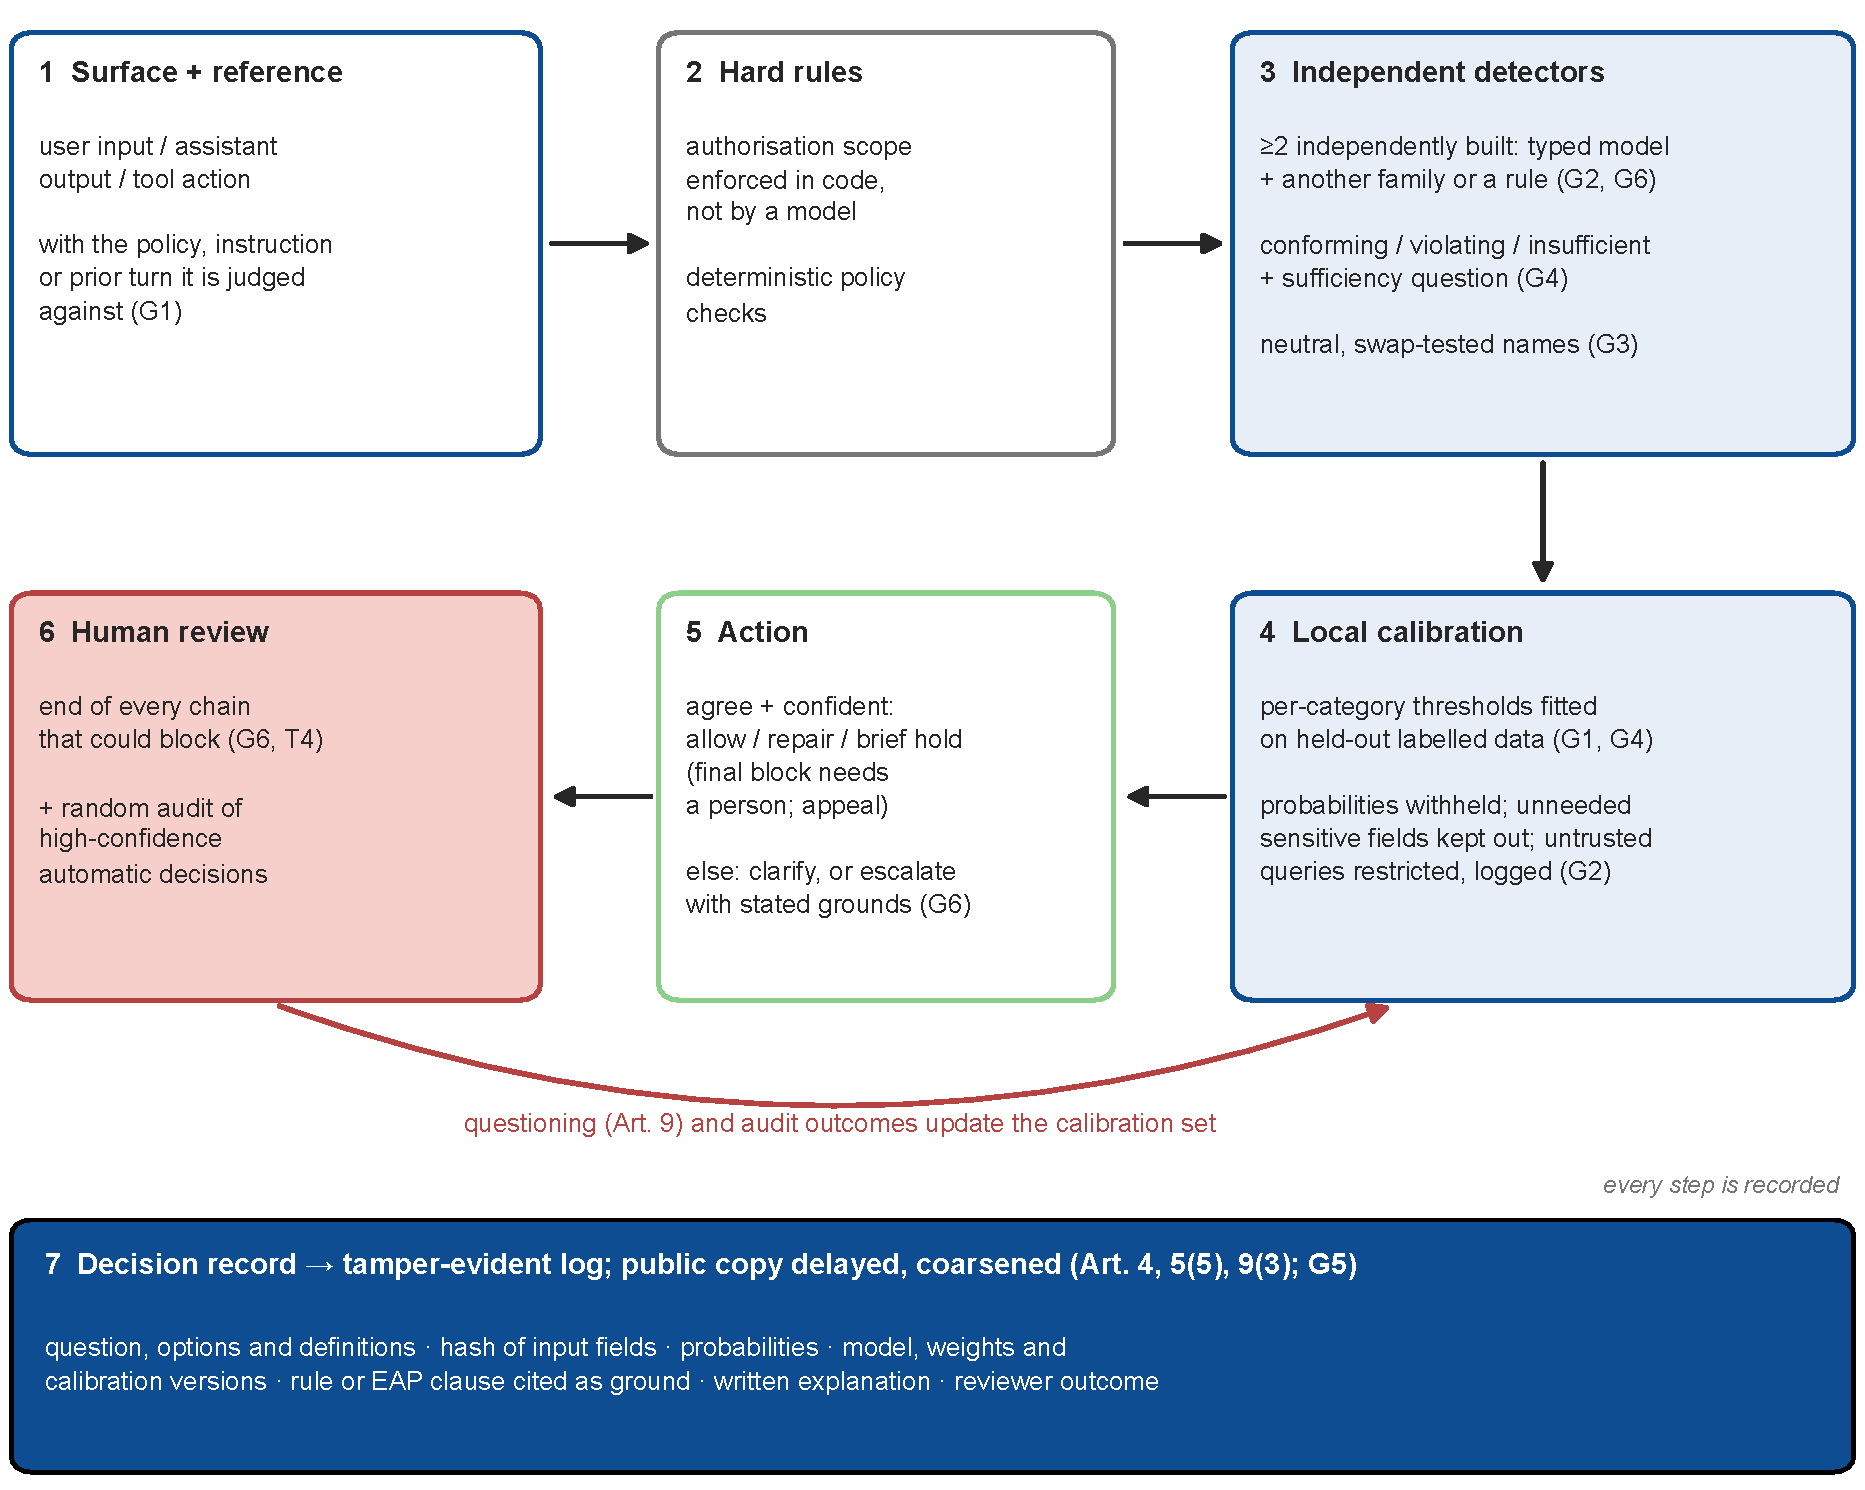
\includegraphics[width=0.8\linewidth]{figures/fig_architecture.pdf}
\caption{受条款约束的安全阀的参考设计。类型化模型作为检测器（3），其输出在任何自动动作（5）之前先经本地校准（4）；分歧与信息不足的情形予以澄清或升级，任何最终阻断均由人确认，高置信自动决策的随机样本由人审计（6）；每一步均写入决策记录（7）。括号中的标签给出促成各要素的要求或张力。}
\label{fig:architecture}
\end{figure}

该设计包含七个要素。
\begin{enumerate}
  \item \textbf{向检测器提供参照，而不仅是文本。} 许多失效是相对于某条指令、某项政策或某个先前陈述而界定的~\cite{arx29429}；受审内容始终与该语境配对提供。需要计算或推理的事实（求和、日期、后果）在代码中或在单独记录的步骤中计算并写入状态，而不交给检测器~\cite{arx39496,arx01834}。
  \item \textbf{在代码中强制执行权限范围。} 智能体是否停留在其授权范围之内，是外围系统的属性~\cite{arx22664}，应在调用任何模型之前通过能力检查强制执行。
  \item \textbf{使用至少两个独立构建的检测器。} 阻断信号要求构造不同的检测器之间取得一致，例如不同模型家族的模型，或一个模型与一条规则，因为同类模型会共享高置信错误~\cite{arx29769}；而与一条不同构造的规则取得一致，使审核者能够跳过约三分之一的案例而不损失 macro-F1，尽管被标记为非良性的伪装攻击有所减少~\cite{arx02048}。每个问题都是三值的（符合、违反、信息不足），充分性也作为单独的是/否问题提出~\cite{arx01006}，选项使用绑定到定义的中性标识符，并须通过重命名测试~\cite{arx26758,arx00346}。必须相互独立失效的标记（放行/阻断、风险等级、是否需要人工）在不同的调用中分别询问，因为在一个与 \jev{} 兼容的开源模型中，一条植入的注释就改变了同一调用中的多个答案~\cite{zen23038928}\zmark{}。在准确性足够之处，优先使用可自托管的模型（T3）。三值判定已是该工作组试点协议的一部分。
  \item \textbf{本地校准，不向不受信任的调用方提供概率，并限制其可查询的内容。} 阈值按类别在留出的本地数据上拟合~\cite{arx29429,arx24052,jkf87_2026replication}，在可交换性假设合理之处采用无分布风险控制~\cite{bates2021distribution,angelopoulos2024conformal}，并对每种新的问题类型重新认证~\cite{arx33689}，同时按既定时间表定期重新认证，且每当时间再验证未通过时（\cref{tab:checklist} 第~16 项）亦予重新认证。原始概率不返回给不受信任的调用方，因为概率有助于攻击者优化攻击，尽管仅凭标签攻击也能得逞~\cite{arx30243,arx28613}；决策所不需要的字段，尤其是敏感属性，不放入检测器的输入，因为一名获得该任务授权的用户通过在输入中植入条件指令，仅凭标签、每个状态两至六次查询即恢复了隐藏属性；不受信任的调用方的查询限于经授权的任务，因为标签曾被用来完善有害计划，且这些查询须予记录，因为标签还曾被用来训练替身模型~\cite{arx04985}。
  \item \textbf{仅在取得一致时自动行动，且对人的限制只能是短暂和可逆的。} 一致加上经过校准的置信度，允许自动\emph{放行}、自动\emph{修复} AI 系统自身的输出（例如 \clause{4.3.3.1} 的恨语截断，但绝不编辑人的消息），以及对人的内容进行有时限（例如至多 24 小时）且完全可逆的\emph{暂扣}。暂扣只有经人确认后，才成为对某人言论、某项福利或某个账户的最终阻断，并始终可以申诉。出现分歧或 \texttt{insufficient} 时，转入澄清，或升级至一个必须陈述其依据的更强推理模型~\cite{arx26550}。由于自动放行对任何受被放行内容伤害的人都具有实质后果，漏检率与误阻断率一并受到监测与治理。正是这一要素使类型化模型保持在\cref{sec:intro} 意义上的检测器角色。
  \item \textbf{每一条可能导致阻断的链路都以人为终点，并审计高置信决策。} 审核者查看每一项将以阻断告终的升级、每一项未解决的升级，以及高置信自动决策的随机样本，因为危害最大的错误是高置信且共享的~\cite{arx29769,arx33401}；审核结果以及依 \art{9} 进行的公众质询的结果，回馈到校准集中。
  \item \textbf{记录每一项决策。} 每条记录包含问题、选项集合与定义、输入字段的哈希值、概率、模型版本、权重版本与校准版本、作为依据援引的规则或条款、任何书面解释，以及审核者的处理结果。记录保存在向监督者开放的防篡改日志中（\art{9}(3)）；公开版本以粗化并延迟的方式发布概率，从而服务于 \art{4} 与 \art{5}(5)，而不致成为攻击者可反复试探的判定接口（oracle）。
\end{enumerate}

\paragraph{使人工复核切实可行。}
链路终点上的人只有在能够胜任这项工作时，才构成保障机制。
审核者需要容量：严格的错误上限会把工作量转移到复核与阻断上~\cite{arx33401}，插入的观点会把高置信答案推入复核~\cite{arx31142}，因此复核负荷必须与准确性一并纳入预算并予以报告，而更低成本的评估可能增加而非减少总负荷~\cite{arx01231}。
审核者容易产生自动化偏差与自满~\cite{parasuraman2010complacency,green2022flaws}，并可能成为系统失效责任的落脚点~\cite{elish2019moral}，因此在随机审计期间应隐藏模型的判定与概率，并测量审核者之间的一致性，而不仅是其与模型的一致性。
人们也恰恰在类型化模型最过度自信的那些有争议条目上意见分歧~\cite{pavlick2019inherent,davani2022dealing,zen23032384}\zmark{}，因此有争议的类别需要不止一名审核者，而受影响的人需要得到通知、理由说明和申诉途径~\cite{santaclara2021,dsa2022}。

\paragraph{本设计的权衡与已知局限。}
要求两个检测器在阻断前取得一致会降低灵敏度：更多违规会被漏检，这与通常靠更多阻断来满足的严格漏检上限相冲突~\cite{arx33401}；本设计转而接受更多暂扣与更多复核，其漏检率必须加以测量。
风险控制的保证以校准数据与部署数据之间的可交换性为前提；它们在良性漂移下而非自适应攻击下约束错误，而 G2 的证据表明自适应攻击是现实的。
就仇恨言论而言，这种分布偏移并非假设：在 20 个语言模型上，四个静态英文仇恨言论基准上的排名并不能预测其在带时间戳数据或新词替换数据上的排名（Spearman $\rho$ 介于 $-0.31$ 与 $0.19$ 之间，所有 90\% 区间均包含零），而各静态基准彼此之间相互一致（平均 $\rho = 0.36$）~\cite{dibonaventura2025hatevolution}。
为独立标记分别调用以及增加第二个检测器，会成倍增加成本与延迟，削弱类型化模型的主要优势，尽管已测得的成本留有很大余地~\cite{arx00346,arx01079}。
最后，大多数要素所依据的证据确定性为低或极低（见\cref{tab:keyfindings}）；本设计是一个有待在 \pol{} 的构念上检验的假设，而非经过验证的系统。

\Cref{tab:checklist} 将证据转化为一份核查清单，适用于任何拟用于此类保障机制的类型化模型。
第 1--4、9、14 和 15 项借鉴了~\cite{arx32160} 的 14 项中的 9 项（其 B1--B2、C1、C3--C4、R1--R2 与 T2--T3）；其余各项为治理保障机制而增设，该清单的 B3、T1、T4、R3 与 C2 未予采用。每一项都有一个暂定的通过标准；这些数值是供部署该保障机制者设定的起点，而非经实证验证的阈值。

\begin{table}[!htbp]
\centering
\footnotesize
\caption{用于治理保障机制中类型化决策模型的评估核查清单及暂定通过标准。“依据”给出相应的证据或条款；标有 $\circ$ 的条目是在~\protect\cite{arx32160} 的核查清单之外增设的。}
\label{tab:checklist}
\begin{tabularx}{\linewidth}{@{}rL>{\raggedright\arraybackslash}p{0.27\linewidth}>{\raggedright\arraybackslash}p{0.17\linewidth}@{}}
\toprule
\# & 要求 & 暂定通过标准 & 依据 \\
\midrule
1 & 与生成式模型的标签概率读出以及低成本生成式级联进行比较 & 在相同条目上报告 & \cite{arx32160} \\
2 & 在留出的本地数据上拟合阈值；报告拟合阈值与默认阈值下的 F1 & 拟合阈值以单侧风险界加以认证 & \cite{arx29429,arx00346} \\
3 & 按类别报告本地重新校准前后的校准情况 & 按类别报告 ECE 与斜率及其区间 & \cite{arx24052,arx27607} \\
4 & 选项名称互换测试 & 定义互换下的翻转率至多为重复噪声下限的两倍 & \cite{arx26758,arx00346} \\
5$^\circ$ & 包括 \texttt{insufficient} 在内的三个选项，外加单独的充分性问题 & 在成对的信息存在/缺失条目上，\texttt{insufficient} 的召回率至少为 0.5 & \cite{arx39496,arx01006,polgov} \\
6$^\circ$ & 互补问题与互斥问题的一致性 & 与总和为一的偏差在重复噪声的两倍以内 & \cite{arx33209} \\
7$^\circ$ & 以自适应的概率引导式添加、插入观点、诱饵与多轮攻击进行红队测试，并在已部署的输入与查询限制下进行仅凭标签的判定接口（oracle）攻击（属性推断、替身模型提取） & 按攻击类型报告攻击成功率，且低于预先设定的目标 & \cite{arx30243,arx31142,arx01834,checkpoint2026jev,arx04985} \\
8$^\circ$ & 按子类型（包括高置信错误）分解错误 & 没有召回率低于设定下限的子类型 & \cite{arx33401} \\
9 & 跨重复、接口与分解方式的决策层面稳定性 & 报告跨接口的分歧；每个问题固定一种接口 & \cite{arx27678,arx37470,arx33971} \\
10$^\circ$ & 与每个升级目标之间的错误相关性 & 高置信错误的重复率低于独立情形加上设定余量 & \cite{arx29769} \\
11$^\circ$ & 以中文及所服务的每种语言进行评估，并包含文字与选项顺序变体 & 每种语言均在英文的设定余量之内 & \cite{qin2026zhdecisionbench,typesafe_models} \\
12$^\circ$ & 不在人群之间进行强制选择；对行为问题进行群体偏见测试 & 各群体的错误率在设定余量之内 & \cite{simmons2026saidno,sap2019risk} \\
13$^\circ$ & 价值负载问题：无人设时的默认立场，以及在人们意见分歧处的表现 & 予以报告；有争议条目交由人处理 & \cite{arx36399,zen23032384} \\
14 & 有无缓存时的延迟；每个正确决策的成本 & 予以报告，包括复核负荷 & \cite{arx32160,arx00346} \\
15 & 版本与可检查性 & 在每条记录中固定模型、权重与校准版本；可自托管或留有记录 & \art{4}、\art{5}(4)--(5)、\clause{5.5} \\
16$^\circ$ & 时间再验证：在由近期条目构成的带时间戳留出集上，以及在将目标词替换为新近出现的同义新词的成对条目上重新评估 & 在所服务的每种语言中（第 11 项）：恨语的分时段召回率在认证时段的设定余量之内，且新词替换句对上的翻转率在重复噪声下限的设定余量之内；任一项超出时，按第 2 项的程序重新认证阈值 & \cite{dibonaventura2025hatevolution}（仅英文；未测试类型化模型） \\
\bottomrule
\end{tabularx}
\end{table}

\section{讨论}
\label{sec:discussion}

\subsection{托管 Jev 是否适合作为 \pol{} 的治理工具？}
\label{sec:verdict}

前述各节以检测器与裁决者之分回答了研究问题。
此处我们逐项功能地说明这一回答对规范本身意味着什么，使该结论能够对照已编码的发现及其确定性（\cref{tab:keyfindings}）加以核查，而非靠推断得出。
\Cref{tab:verdict} 列出类型化模型可能被要求承担的每一项 \pol{} 功能，指明其所涉及的要求，给出决定该功能结论的一两项发现，并给出三种结论之一：\emph{证据不支持}，即已编码证据显示该功能失效，或该功能依赖于证据所否定的某一属性；\emph{仅作有条件的检测器}，即该功能可以在 \cref{sec:design} 的设计之内、以 \cref{sec:intro} 所述的检测器角色、作为留有记录的检测器履行，而证据不允许以其他任何方式履行；\emph{未经测试}，即没有已编码研究测量该条款在 \pol{} 构念上所要求的内容。
每一个确定性条目均为相应发现在 \cref{tab:keyfindings} 中的评级；没有一项为中等，凡依赖有争议发现的结论均作了相应标记。
这些结论针对的是 2026 年 9 月 15 日至 10 月 8 日各版本的托管 \jev{}，并在发现的适用范围为“两者”之处，针对一般类型化模型；它们不是对后续模型的预测。

{\scriptsize
\setlength{\tabcolsep}{3pt}
\begin{longtable}{@{}>{\raggedright\arraybackslash}p{0.12\linewidth}>{\raggedright\arraybackslash}p{0.04\linewidth}>{\raggedright\arraybackslash}p{0.34\linewidth}>{\raggedright\arraybackslash}p{0.14\linewidth}>{\raggedright\arraybackslash}p{0.10\linewidth}>{\raggedright\arraybackslash}p{0.17\linewidth}@{}}
\caption{逐项功能的 \pol{} 结论。\emph{要求}：所涉及的 \cref{tab:clauses} 中的要求。\emph{证据}：决定该结论的已编码发现及其决定性数字。\emph{结论}：NS，证据不支持；DC，仅作有条件的检测器，且须留有记录（即 \cref{sec:design} 的设计）；NT，未在 \pol{} 的构念上经过测试。同一单元格可对某项功能的一部分给出 NS、对另一部分给出 NT；“审慎原则”标记的是依据测量缺失、而非依据测得的失效所作的限制（\cref{sec:scope-certainty} 的规则）。\emph{确定性}：决定性发现在 \cref{tab:keyfindings} 中的评级；$^{c}$~有争议；“未评级”标记并非关键发现、且依赖单项研究的结果。所有评级均为低或极低。}
\label{tab:verdict}\\
\toprule
\pol{} 功能 & 要求 & 证据显示的内容 & 结论 & 确定性 & 尚需什么 \\
\midrule
\endfirsthead
\multicolumn{6}{@{}l}{\emph{\Cref{tab:verdict}（续）。}}\\
\toprule
\pol{} 功能 & 要求 & 证据显示的内容 & 结论 & 确定性 & 尚需什么 \\
\midrule
\endhead
\bottomrule
\endlastfoot
安全阀：阻断输入中的恨语（\clause{5.4.1}） & G1, G2, G3, G6 &
零样本下对有害英文内容的排序效果良好（中位 AUROC 0.886，每轮成本 \$0.30，对照为 \$18.96~\cite{arx29429}），在 HateCheck 诊断集上与一个前沿 LLM 的 macro-F1 相差不超过 1.6 个点，成本低 97\%~\cite{arx03324}；但固定阈值失效（阈值 0.5 时 F1 为 0.158，拟合阈值下为 0.947~\cite{jkf87_2026replication}），一种针对 \jev{} 的注入与一种通用后缀达到 97--100\% 的攻击成功率~\cite{arx04985}，一条插入的观点翻转了 12.1\% 的决策~\cite{arx31142}，互换选项定义改变了 32.5--50.5\% 的答案~\cite{arx26758,arx00346}。 &
DC：仅在独立构建的检测器取得一致时自动\emph{暂扣}；最终阻断由人作出 &
低（排序；操纵；选项名称）；低$^{c}$（阈值） &
一个中文三值基准；在本地留出数据上认证并随时间重新认证的阈值；每类攻击的红队成功率低于预先设定的目标；通过重命名测试的中性标识符 \\
\addlinespace
输出抑制：对 PAI 自身输出的恨语截断（\clause{4.3.3.1}） & G1, G3, G5 &
所有系统对仇恨语言与仅具冒犯性语言的区分都很弱（三分类 macro-F1：\jev{} 0.532，前沿 LLM 0.604，有监督 TF-IDF 0.639~\cite{arx03324}）；在没有检索先例的情况下，准确选出被违反的仇恨言论政策的比例为 29.4\%~\cite{arx07953}；错误集中于总体指标所掩盖的子类型（167 次漏检中有 130 次的置信度 $\geq 0.95$~\cite{arx33401}）。 &
DC：自动\emph{修复} AI 自身的输出是可逆的，且处于检测器角色之内；截断记录必须显示被删除的内容 &
低（子类型；选项名称）；低（排序） &
以中文测得的恨语相对于冒犯性语言及不在场状态的召回率；子类型召回率下限；每次截断的记录，向其所针对的人开放 \\
\addlinespace
实时矫正支持：识别与矫正建议（\clause{4.3.3.2}） & G1, G5 &
识别见上一行。类型化决策只返回一个概率，别无其他~\cite{willison2026jev}，因此矫正\emph{建议}需要一个生成式组件，而其依据并非该判定的依据（\cref{sec:g5}）；在中文情绪分类上，所有系统均表现较弱（macro-F1：\jev{} 21.06，生成式模型 19.82--23.31~\cite{arx08829}）。 &
NT：类型化接口仅涵盖识别；建议未经测试 &
低（排序）；未评级（中文情绪，单次运行） &
一项中文测试，检验在类型化判定之后生成的建议是否反映了产生该判定的因素 \\
\addlinespace
异常检测与风险预警（\art{7}(2)--(3)） & G1, G2, G6 &
在文本上，是附带上述条件的检测器；在非文本信号上，零样本 \jev{} 在网络流量特征上的得分低于多数类基线（9.8\% 对 22.8\%~\cite{arx00376}），在工业故障检测中将 57--94\% 的无故障窗口标记为异常，且在分布偏移下并不优于将每个窗口都标记为异常~\cite{arx09937}；伪装为正常运行的攻击召回率为 0.34，被一致性门控接受为良性的 76 个窗口中有 21 个是攻击~\cite{arx02048}。 &
文本上为 DC；在没有经训练模型的情况下，对数值或结构化信号为 NS &
低（子类型；操纵）；极低（一致性门控） &
以规范自身术语给出的“异常模式”定义；漂移与伪装攻击测试；以经训练的或基于规则的检测器作为独立的第二道核查 \\
\addlinespace
对齐的伦理验证（\art{6}(3)） & G3, G4, G5 &
在无人设时，\jev{} 回答价值问题的方式与其美国人设相似，沙特人设在英文中重现了人类沙特--美国差异的 87\%，在阿拉伯文中则为 62\%~\cite{arx36399}；在道德两难问题上，改写措辞对其答案的影响远大于重复运行~\cite{zen23023694}\zmark{}；在标注者分歧最大之处，其校准误差升至 0.339~\cite{zen23032384}\zmark{}，并且在人们以 55 比 45 分歧的条目上报告了 0.88~\cite{zen23179064}\zmark{}。 &
作为自动验证器为 NS，因为它依赖于中性的默认立场以及在人们存在分歧之处的校准，而两者均被证据否定；EAP 构念本身为 NT &
极低（文化）；低（校准是局部的） &
一个由价值负载的 \pol{} 问题构成、采用顾及分歧标签的基准，报告其无人设时的默认立场，并将有争议条目交由人处理 \\
\addlinespace
无需人工干预的争议裁决（\art{10}，\art{9}(7)） & G4, G5, G6 &
低成本同类评估器在 96.0\% 的判定中重复了 \jev{} 置信度最高的错误（上界）~\cite{arx29769}，并在 130 次高置信漏检中至多发现 5 次~\cite{arx33401}；明确的“不知道”选项在其为正确答案的条目中有 10.5\% 被选中，“以上皆非”（None）为 7--54\%~\cite{arx34024,arx39496}；通过两种接口提出的同一决策在 32.8\% 的情况下导致不同行动~\cite{arx37470}；预先固定的阈值在 14 项任务中的 8 项上未达到其准确率目标~\cite{arx24574}，一项预注册研究使这一发现有争议~\cite{arx33689}；输出不附带理由~\cite{willison2026jev}。 &
作为裁决者为 NS；仅对申请的排序与分诊为 DC &
低（同类模型错误；“不知道”）；低$^{c}$（预先设定的阈值） &
下文“何种情况会改变结论”中的四项条件，在一个中文 \pol{} 基准上，于一项经预注册并有独立重复的研究或两项独立研究中得到满足 \\
\addlinespace
对爱语与恨语的逐人量化（\clause{5.6}） & G3, G7 &
在一项非正式的强制选择测试中存在群体偏倚（“White”占首选的 51\%~\cite{simmons2026saidno}\gmark{}）；类型化与生成式模型在低资源语言上均出现性能退化~\cite{arx37647}；第三方插入的观点翻转了 12.1\% 的决策~\cite{arx31142}，因而汇总结果可能被操纵；没有研究测量行为判断中按说话者群体区分的差异化错误。 &
作为决策输入为 NS（操纵，低）；按群体的错误为 NT：在按群体与语言的错误公布之前，只对事件与行为评分，绝不对人评分（审慎原则，\cref{sec:scope-certainty}） &
极低（文化）；低（操纵）；未评级（群体偏倚，单项非正式测试；语言退化，单一基准） &
以中文公布的按群体与语言划分的错误率；同意、查阅本人记录与申诉；对照社会评分禁令的法律解读（\cref{sec:synthesis}，T5） \\
\addlinespace
公共决策中的评估维度（\clause{5.6}） & G7 &
总体规模的解读可以诚实地完成：一个人类--模型共享误差项在名义 80\% 与 90\% 水平下给出了 0.93 与 0.96 的回顾性覆盖率~\cite{arx27535}，经审计的概率样本给出了校正后的全州计数，但仅在按因素进行人工再校准之后~\cite{arx00213,arx10321}；模拟公众偏向某一人群~\cite{arx36399}，并低估分歧~\cite{zen23179064}\zmark{}。 &
DC：作为经审计的汇总测量，其测得误差须带入每一项结论；本身不作为决策输入 &
极低（文化）；未评级（审计设计，单项研究） &
一个由真实 \pol{} 条目构成、顾及分歧的审计样本；每一项估计都报告其与人之间的测得差距 \\
\end{longtable}
}

\paragraph{结论。}
按截至 2026 年 10 月 8 日的证据，托管 \jev{} 不适合承担 \pol{} 中任何“做决定”的功能。
这包括 \art{10} 下的争议裁决、\art{6}(3) 下的自动伦理验证、\clause{5.6} 的逐人量化（依据在于操纵，以及任何群体错误测量的缺失），以及安全阀的任何如下用法：对某人言论的阻断无须经人确认即成为最终结果。
决定性的发现是否定性的，并且在其低或极低的确定性范围内相互一致：在一种情境中拟合的阈值不能迁移到另一种情境（低，有争议）；决策可被模型所审计对象内部的内容操纵（低；定制注入的攻击成功率为 97--100\%~\cite{arx04985}，一条插入的观点翻转了 12.1\% 的决策~\cite{arx31142}）；选项名称可能压过其定义（低）；明确的“不知道”选项在其为正确答案时很少被选择，“以上皆非”的选择则不一致（低）；而此类模型会升级至的低成本评估器重复了其几乎全部高置信错误（低，上界）。
具有这些特性的裁决者，将依据可被对手操纵、取决于问题措辞、且很可能没有第二个自动意见能够发现的判定来限制言论、分配福利；\art{9}(7) 使人的监督不得干预，这将移除证据表明所必需的唯一一道核查。
所测试的类型化模型无一能逃脱这一结论，与之一同测试的低成本生成式评估器也未被证明能够逃脱：在进行了比较之处，类型化模型并非普遍更差（低，依据判断），但大多数失效从未进行比较，因此该结论并非专属于类型化模型，并且在生成式评估器于同一协议下接受检验之前，出于审慎原则适用于这一成本层级的自动裁决者（\cref{sec:scope-certainty}）。

对于检测而非决定的功能，即 \clause{5.4.1} 的安全阀、\clause{4.3.3.1} 的截断，以及 \art{7} 在文本上的异常检测（不包括在没有经训练模型时对数值或结构化运行信号的检测，\cref{tab:verdict}），托管 \jev{} 可以使用，但只能在 \cref{sec:design} 的设计之内使用；\clause{5.6} 的公共决策评估仅可作为经审计的汇总测量使用，并须将其测得误差带入每一项结论；支持这一点的正面证据是真实的，但附有条件。
它以生成式评估器成本的一小部分对有害英文内容作出良好排序（低），在 HateCheck 诊断集上与前沿模型的 macro-F1 相差不超过 1.6 个点，成本低 97\%~\cite{arx03324}；它在与其训练相似的任务上往往校准良好（低）；基于置信度的暂缓判定在分布内有效~\cite{arx00381,zen22885291}；在一项预注册研究中，仅在一条独立构建的规则同意时才接受其低风险判定，并未损失 macro-F1，尽管伪装攻击得以通过（极低）。
每一项正面证据都附有将其转化为设计要素的条件：排序在成为决定之前需要经本地拟合并重新认证的阈值；校准只在测得之处成立；暂缓判定只在分布内成立；一致性门控需要一个构造不同的第二检测器。
即便这一检测器结论也是一种外推：它依据的是二值仇恨言论的英文基准，而 \pol{} 要求以中文对爱语、恨语与不在场状态作出三值判断，且没有已编码研究测量这一构念；唯一的中文情绪结果显示所有系统均较弱（macro-F1 约为 21~\cite{arx08829}），仅有的中文决策基准涉及服务路由、诈骗检测与船舶设计工程，而非恨语~\cite{qin2026zhdecisionbench,arx09896}；而仇恨语言与仅具冒犯性语言的区分，即 \clause{1.5} 最需要的区分，在所有受测系统中都很弱~\cite{arx03324}。
因此，我们在陈述结论时附上其确定性：上述每一项发现均为低或极低，四项有争议，大多数依赖单一团队在模型面世最初几周内发布的预印本，而一项针对该规范自身构念、设计良好的研究即可能改变这些评级。

另有两项发现与 \pol{} 的关联超出任何单一功能。
类型化保障机制也可能充当可查询的判定接口（oracle）：在输入中植入条件指令后，仅凭托管 \jev{} 的标签，就在每一个测试案例中揭示了隐藏的性别、年龄组、心脏病与族裔属性，每个状态需两到六次查询（开源模型的标签未揭示任何属性）；此外，其判定提高了有害计划被评判的有害程度，其标签以 200 个标签训练出一个一致率达 92\% 的替身模型~\cite{arx04985}。这支持不向不受信任的调用方提供安全阀的概率，并将决策不需要的敏感字段排除在输入之外；对托管 \jev{} 而言，后者是这些措施中唯一能够消除该信号的一项，因为该攻击对获授权执行该任务的用户同样有效，且仅需标签；将不受信任调用方的查询限制在获授权的任务之内，可防止安全阀成为回答诸如有害计划可行性等问题的通用判定接口，而日志记录可使通过获授权任务进行的替身模型提取变得可见，但两者都不能阻止这种提取（\cref{sec:design}，要素~4）。这些措施均未经测试。
另外，一个封闭的托管模型无法按其字面要求满足 \art{4} 与 \art{5}(4)（T3）：其决策记录可以公开，其推理则不能；而与开源模型测得的鲁棒性之间的权衡（开源模型表现出最严重的名称反转~\cite{arx26758}）必须明确作出。

\paragraph{可借鉴之处。}
有若干经验无论使用何种模型都适用于 \pol{}，因为每一条都源自一项关乎接口或任务、而非关乎 \jev{} 的发现。
\begin{itemize}
  \item \emph{提出三值问题，并单独询问充分性。} 是/否问题会丢弃不在场状态（\clause{4.3.2}）；明确的“不知道”与“以上皆非”选项的选择并不一致（低），但在一项研究中，单独就证据是否充分提出的是/否问题，比置信度更能发现信息缺失~\cite{arx01006}（极低）。三值判定已纳入该工作组的试点方案~\cite{polgov}（\cref{sec:design}，要素~3；T2）。
  \item \emph{将中性标识符绑定到定义，并通过重命名加以测试。} 对所有受测类型化模型，选项名称都压过了定义（低），而数字或随机字符串标识符使托管 \jev{} 接近其噪声下限~\cite{arx00346}；\clause{1.5} 指出其概念并非道德词汇，道德词汇应置于定义之中，而不应置于选项名称之中（要素~3；核查清单第~4 项）。
  \item \emph{记录每一项决策。} 类型化判定不附带理由（\cref{sec:g5}），因此记录（问题、选项集及定义、输入哈希、概率、模型与校准版本、所援引的依据、复核结果）是依 \art{9} 唯一可被审计或质询的对象，也是 \art{5}(5) 可验证的决策链路的唯一基础（要素~7）。
  \item \emph{在本地校准，并随时间重新验证。} 在别处拟合的阈值未能迁移（低，有争议），校准是局部的（低）；静态基准上的仇恨言论排名不能预测在带时间戳或经新词替换的数据上的排名~\cite{dibonaventura2025hatevolution}，因此认证有其日期与语言（要素~4；核查清单第 2、3、11 与 16 项）。
  \item \emph{仅在构造不同的检测器取得一致时才触发自动动作。} 同类模型重复了高置信错误（低）；仅在一条独立构建的规则同意时才接受判定，并未损失 macro-F1，但伪装攻击仍然通过（极低），因此独立性必须被构建而不能被假定，且须测量其漏检率（要素~3；核查清单第~10 项）。
  \item \emph{凡可能限制人的链条，均以人作为终点，并审计高置信决策。} 最具破坏性的错误是高置信且共有的~\cite{arx29769,arx33401}，且没有研究在治理条目上将类型化模型与受训审核者进行比较；在此类研究出现之前，带有盲法随机审计的人工终点是证据未予削弱的唯一核查（要素 5 与 6；T4，选项~(b)）。
  \item \emph{不向不受信任的调用方提供概率，将不需要的敏感字段排除在输入之外，限制并记录不受信任的查询，并将相互独立的标记拆分到不同的调用中。} 概率反馈帮助了攻击者~\cite{arx30243}，仅凭标签即泄露了属性并训练出替身模型~\cite{arx04985}，一条植入的注释在一次调用中改变了多个答案~\cite{zen23038928}\zmark{}（要素 3 与 4）。
  \item \emph{在按群体与语言的错误公布之前，只对事件与行为评分，绝不对人评分。} 这既源自证据，同样也源自 \clause{4.3.1}（T5）。
  \item \emph{首先构建构念基准。} 上述每一项结论都是从英文二值任务外推而来；一个经独立标注、顾及分歧、带时间戳、以中文标注爱语、恨语与不在场状态并设有留出集的基准，是将其中任何结论从外推转为测量的前提（见下文开放问题）。
\end{itemize}

\subsection{范围、确定性、局限性与开放问题}
\label{sec:scope-certainty}

\paragraph{超越单一规范。}
任何在 AI 系统之前设置自动过滤器、将争议交给 AI，或为公共目的对人的行为进行评分的提案，都面临 G1--G7 这些问题；并且，在下文关于确定性的保留之下，\cref{sec:design} 的设计结论很可能也适用于它。
\cref{sec:paradigms} 中的比较使这一点具体化：宪法分类器、中国关于停止违法生成的义务以及 DSA 关于自动化手段的条款，都在朝推理期拦截层的方向推进，随后各自都需要回答 G1--G5，并在其将监督自动化之处回答 G6 的升级问题，而其自身文本对这些问题至多只给出了部分回答（《生成式人工智能服务管理暂行办法》要求记录对用户采取的措施并设立投诉渠道，第 14 条第 2 款与第 15 条~\cite{cac2023genai}）；G7 与 G6 的其余部分只在某一提案同时将争议交给 AI 或对人评分时才会出现。
本案例的增益在于表明：一份治理文本可以逐条解读为一组可检验的要求，而这样做会暴露出在仅把文本当作价值宣言来阅读时无从察觉的张力。
在本案例中，该框架自身的若干承诺，即不在场状态、关于爱与恨并非道德标签的告诫，以及对人与行为的区分，与证据所推荐的做法相一致；张力出现在其他条款与之相拉扯之处。

\paragraph{确定性。}
\Cref{tab:keyfindings} 对摘要与结论中使用的每一项发现进行了评级。
这些规则计入与某项发现相关的每一项已编码研究，将有共同作者的研究计为一项，只承认其他团队基于自身数据或重新实现所作的研究为独立重复，按系统组计数证据，并仅依据托管模型证据对关于托管 \jev{} 或一般类型化模型的发现进行评级（开源模型研究仅作佐证），且当一项设计强度至少相当的研究指向相反方向时降低评级（\cref{sec:appraisal}）；每项已编码研究在各项发现中的归属均已发布（\nolinkurl{data/certainty_evidence.csv}），评级由 \nolinkurl{scripts/rate_certainty.py} 据此计算得出。
这些规则在第 12--15 轮审查期间、即更新研究完成编码之后，根据审查者的意见作了修订，所有发现均据此重新评级；这偏离了曾冻结主窗口评级的更新方案，因此该表在当前评级旁列出了 10 月 4 日给定的评级。
没有发现达到中等确定性。若开源模型研究可以提高评级，“插入内容会操纵判定”将为中等；而在我们的规则下，它们只起佐证作用。
有四项发现有争议：注入很少选中攻击者的目标，评级为极低；升级至更强的推理模型可在不损失准确率的情况下节省成本，评级为低；以及两项阈值发现，即固定阈值不可迁移、预先设定的阈值在新数据上达不到其错误目标，评级为低。这两项均得到一项预注册研究的支持，在该研究中，预先固定的阈值在 14 项任务中的 8 项上未达到其准确率目标~\cite{arx24574}，并得到若干其他 \jev{} 研究的支持；两项均受到一项关于问题类型变化的预注册研究的反对，在该研究中，\jev{} 预先设定的门控在 7 个模板中的 6 个上保持在其目标之内~\cite{arx33689}，第二项还受到两项阈值达到目标的更新研究的反对~\cite{zen22935043,zen23075657}\zmark{}；由于该预注册相反研究与最强的支持研究同级，两项均由中等降为低。
所有评级均为低或极低，原因在于来源是模型发布后数日内发布的预印本，许多结果仅依赖一项研究，对一项重点研究的唯一一次再现重跑的是其作者的代码与数据，且没有研究测量该规范自身的构念。

\paragraph{局限性。}
语料库涵盖十七天内的投稿，由未经同行评审的预印本与灰色文献组成，其中许多出自快速工作的单一作者；在一个社区追踪项目评级的 27 项早期研究中，没有一项被评为低偏倚风险~\cite{rafe2026awesome}。
关于失效的研究在模型面世的最初几周内易于撰写，因而可能被过度代表；Zenodo 记录比 arXiv 论文更常给出否定结果，尽管剔除它们对总体比例的影响很小（见\cref{sec:across}）。
若干研究使用的是开源模型而非托管模型，有些研究未报告托管模型的版本；我们每次都予以说明，但计票结果将托管模型与开源模型合并统计。
各项要求源自 \pol{}，因此本分析回答的是它的问题，可能遗漏类型化模型在其未提出的问题上的长处。
筛选、提取、编码与核验均由 AI 智能体在作者指导下完成，且两名编码者是同一模型家族的 AI 智能体，因此一致性统计量（$\kappa = \nKappa{}$，95\% CI \nKappaLo{}--\nKappaHi{}，样本以 Q 编码为主）是该编码手册对人类编码者可重复程度的上界；对全部更新配对的全量编码得到 $\kappa = \nUKappa{}$（95\% CI \nUKappaLo{}--\nUKappaHi{}），其区间与前者重叠，是对 AI 编码者而言更好的估计，这意味着主窗口中只编码一次的编码有一部分在第二次审读时会得出不同结论。
主计数涵盖截至 10 月 4 日检索到的记录，且主检索的查全率并不完整：在日期位于窗口内的 103 项已编码研究中，有 18 项仅由 10 月 8 日的更新检索发现（\cref{sec:update}）；更新检索的结果单独报告、未予合并，其中包括 \nUSetReScreened{} 条无法确认此前曾被排除或遗漏的 Zenodo 记录；10 月 8 日之后公布的论文未予纳入。
没有研究在治理任务上将类型化模型与受过训练的人类审核者进行比较，因此我们无法判断其错误是否比它所协助的人更糟。

\paragraph{何种情况会改变结论。}
如果在一个留出的、经独立标注的中文三值 \pol{} 基准上，一个采用风险控制阈值的类型化模型
（i）将其误阻断率与漏检率保持在部署责任方预先设定的目标之内，
（ii）在名称与定义互换下改变的答案少于其重复噪声下限的两倍，
（iii）在单一观点插入和 64 次查询的自适应攻击下翻转的决策少于 5\%，并且
（iv）与一个独立的受训审核者小组之间的一致程度，至少不低于这些审核者彼此之间的一致程度，
且上述结果见于一项经预注册并有独立重复的研究，或见于两项独立研究，我们将修正“非裁决者”的结论。
如果在这样的基准上，其 AUROC 低于 0.75，或两个独立构建的检测器相互重复了对方 80\% 以上的高置信错误，或在经认证的阈值下复核负荷超过了为之预算的审核者容量，我们将修正“检测器”的论断。
放宽一项保障机制所需的证据，应多于增设一项保障机制所需的证据，因为错误地移除一项保障机制会限制人的言论与资源，而错误地增设一项保障机制只耗费复核时间。
如果在同一基准上，受训审核者与独立小组的一致程度低于经门控的检测器集成，或在超过预设比例的审计案例中将其判定向模型所显示的判定靠拢，我们将修正“具有实质后果的决定最终由人作出”这一建议。
而如果在同一协议下检验的生成式评估器在类型化模型未通过之处通过检验，结论将变为专属于类型化模型；在此之前并非如此。

\paragraph{开放问题。}
\begin{itemize}
  \item \emph{一个 \pol{} 基准。} 目前没有公开数据集对爱语、恨语与不在场状态进行标注。一个经独立标注的中文基准，采用顾及分歧的标签~\cite{davani2022dealing}，参照现有中文冒犯性语言资源的模式构建~\cite{deng2022cold,lu2023toxicn}，并将留出集保存在任何代码仓库之外，是上述每一项建议的首要前提；该工作组公开的 20 个试点条目明确不作为排名集~\cite{polgov}。由于静态的仇恨言论基准会随语言变化而失去预测价值~\cite{dibonaventura2025hatevolution}，此类基准应标注时间戳并定期更新，包括含有新出现词语的配对条目。
  \item \emph{人类审核者与类型化检测器的比较}，在相同的治理条目上进行，包括审核者彼此之间的一致性及其受模型判定影响的程度。
  \item \emph{失效的对照比较。} 大多数否定性发现没有生成式对照；在加入对照的情况下重新运行这些研究，将显示哪些失效是类型化模型所特有的。
  \item \emph{可查询保障机制的鲁棒性。} 隐藏或粗化概率、添加噪声、限制调用频率、将查询限制在获授权的任务之内，或将敏感字段排除在输入之外，能否降低攻击成功率，以及会给合法用户带来多大代价，尚未得到测量。
  \item \emph{忠实的解释。} 由另一模型事后撰写的解释能否反映产生类型化判定的实际因素，需要专门评估，方能满足 \art{9}(2) 的要求。
  \item \emph{逐人度量。} 若实施 \clause{5.6}，则在计算或存储任何逐人度量之前，必须先测量跨群体与跨语言的差异化错误。
  \item \emph{重复研究。} 大多数发现依赖于单一团队的单一研究；基于新数据的独立重复研究（对 \emph{Just Ask Jev} 的再现重跑的是作者的代码与数据~\cite{jkf87_2026replication}）几乎对每一项要求而言都是最有价值的下一步贡献。
\end{itemize}

\section{结论}
\label{sec:conclusion}

我们对 \pol{} 的结论是明确的，并且依现有证据，对每一项作出决定的功能均为否定（\cref{sec:verdict}）。
托管的 \jev{} 及与其一同测试的类型化模型，以及出于审慎原则，与它们一同测试的低成本生成式评估器（尚未表明它们能避免这些失效，且其中多数失效从未经过比较），都不应依 \art{10} 裁决争议、依 \art{6}(3) 自动进行伦理验证、依 \clause{5.6} 量化个人，或使对某人言论的阻断成为最终决定；原因在于：阈值无法迁移，判定可能被其所审计的内容所操纵，并可能取决于选项名称而非定义，明确的“不知道”选项在其为正确答案时很少被选择，而“以上皆非”的选择不一致，并且此类模型所要升级至的同类评估器几乎重复了其全部高置信错误；对于逐人量化，这一结论还基于审慎原则，因为尚无研究按说话者群体测量误差。
对于检测类功能，即 \clause{5.4.1} 的安全阀、\clause{4.3.3.1} 的截断以及 \art{7} 针对文本的异常检测（若无经过训练的模型，则不适用于数值或结构化信号），托管的 \jev{} 只能在\cref{sec:design}的设计中作为有记录、三值、经本地校准的\emph{检测器}使用；在该设计中，自动行动须以独立构建的检测器之间取得一致为前提，对个人的任何限制均为短暂、可逆的，每一条可能导致阻断的链路都以人为终点，高置信的自动决策须受审计，且每一项决策均予记录；\clause{5.6} 的公共决策评估也只能在同样意义上使用，即作为一种经审计的汇总测量，并将其测得误差带入每一项结论。
即便是这一检测器结论，也是从二值仇恨言论的英文基准外推而来的：尚无研究在中文中测量该规范的三值构念，所找到的唯一一项中文情绪结果显示所有系统均表现较弱，而所测试的每一个系统对仇恨言论与仅具冒犯性的语言的区分能力都较弱。
支撑这些结论的每一项发现的确定性均为低或极低，其中四项发现有争议，截至 10 月 8 日的更新检索未推翻其中任何一项；一项针对该规范自身构念、设计良好的研究即可改变其中任何一项。

尽管如此，类型化决策模型的出现带来了自动化治理保障机制所需的接口：对每一次输入与输出给出带概率的类型化判定，且成本低到足以支撑全面筛查。
无论采用何种模型，本评估中可借鉴到 \pol{} 的，是一组与该接口相关的做法：三值问题，并单独询问充分性；绑定到定义并经重命名检验的中性标识符；记录每一项决策；本地校准并进行时间再验证；以构造不同的检测器之间取得一致作为门控；以人为终点的链路，以及对高置信决策的盲法审计；不向不受信任的调用方提供概率；不需要的敏感字段不放入输入，不受信任的查询受到限制并予记录；独立标记在不同调用中分别询问；对事件而非对人评分；以及，在上述任何一项能够被测量而非外推之前，一个中文构念基准。

就 \pol{} 而言，该框架自身的若干承诺与证据所建议的做法一致：不在场状态、关于爱与恨并非道德标签的告诫，以及对人与行为的区分。
另一些条款则被证据凸显为文本尚待作出的选择：是否在理解语言中的情绪与推断个人的情绪状态之间划出明确界线；如何向不能可靠地回答“信息不足”的模型提出三值问题；如何协调透明性与封闭模型；对于具有实质后果的决定，非干预原则是否应让位于能够暂停这些决定的人，这接近于数据保护法在其适用范围内的要求；以及逐人评估能否与平等联结相调和。
将这些选择明确化，并在该规范自身的构念上检验由此形成的保障机制，是后续的工作。

\section*{立场声明与利益冲突}
\label{sec:statements}
\addcontentsline{toc}{section}{立场声明与利益冲突}
作者是 \pol{} 文本所列贡献者之一，并参与 NaturalDAO 治理工作组的工作，本文所讨论的试点协议即出自该工作组；作者在该项工作及该框架上存在声誉利益。
\cref{sec:design}中的若干建议与该试点协议中已作出的选择相吻合，每一处此类吻合均已标明，以便读者判断其究竟是由证据还是由先前设计所驱动。
为限制这一立场的影响，本分析采用在支持性结论与否定性结论之间对称的编码手册，对每一项编码研究进行质量评价，为每一项核心结论报告确定性，为每一项张力提供至少一个保留原文的选项，列出对此前数据集版本的更正，并公开全部编码及其理由。
张力分析在发布前未经框架提出者或其他贡献者审阅。
作者与 TypeSafe AI 及本文讨论的任何模型的开发者均无经济关系。

\section*{AI 辅助的使用}
\addcontentsline{toc}{section}{AI 辅助的使用}
AI 智能体（Claude Opus 5.5，Anthropic）执行了检索、筛选、全文信息提取、编码、质量评价、第二编码、图表脚本编写和初稿撰写，并由同一模型的全新智能体在独立的审阅轮次中依据来源对文本进行核查；智能体的指令、发现及处理结果随数据一并公开。
作者主导了这项工作，确定了研究问题、要求和编码手册，并对全部内容负责；在本次发布之前，作者未亲自对单项编码进行重新编码或复核。

\section*{致谢}
\addcontentsline{toc}{section}{致谢}
作者感谢 NaturalDAO 的陈昌春、邓雯慧、周朝晖和吴文博提出的意见和建议，并感谢 NaturalDAO 代码库的贡献者提供了开放的、带版本管理的 \pol{} 文本，本分析即以此为基础。

\section*{数据与代码可获得性}
\addcontentsline{toc}{section}{数据与代码可获得性}
补充材料（补充材料 S1--S5：条款对照、证据表、研究目录、更正与确定性评级，以及编码手册、检索与筛选）为单独的 PDF，见 \url{https://github.com/naturaldao/NaturalDAO/blob/main/PoL-Governance/research/PoL2-Jev-Typed-Literature-Survey/paper/zh/supplement_zh.pdf}；英文版亦作为 arXiv 投稿的附属文件提供。
文献目录（\nolinkurl{data/papers.csv}、\nolinkurl{data/zenodo_preprints.csv}、\nolinkurl{data/grey_literature.csv}）、证据编码（\nolinkurl{data/evidence_coding.csv}）、质量评价（\nolinkurl{data/quality_appraisal.csv}）、编码者一致性数据（\nolinkurl{data/coder_agreement.csv}）、排除记录（\nolinkurl{data/excluded_records.csv}）、10 月 8 日的更新检索数据（\nolinkurl{data/papers_update_2026-10-08.csv}、\nolinkurl{data/evidence_coding_update_2026-10-08.csv}、\nolinkurl{data/quality_appraisal_update_2026-10-08.csv}、\nolinkurl{data/coder_agreement_update_2026-10-08.csv}、\nolinkurl{data/excluded_records_update_2026-10-08.csv}、\nolinkurl{data/search_rerun_2026-10-08.csv}、\nolinkurl{data/search_rerun_zenodo_2026-10-08.csv}、\nolinkurl{data/search_rerun_2026-10-08_query_hits.csv}）、确定性证据（\nolinkurl{data/certainty_evidence.csv}，即每项编码研究按系统组对每项关键结论的归属）及计算并核查确定性评级的脚本（\nolinkurl{scripts/rate_certainty.py}）、检索脚本、审阅与审计日志、参考文献核验日志、图表脚本以及 LaTeX 源文件，均以 CC0~1.0 许可发布于 NaturalDAO 代码库（\nolinkurl{https://github.com/naturaldao/NaturalDAO}）的 \nolinkurl{PoL-Governance/research/PoL2-Jev-Typed-Literature-Survey} 目录中。
全文仅对采用知识共享（Creative Commons）许可的论文进行再分发，并保留其原始许可；其余论文仅提供链接。

\bibliographystyle{unsrtnat}
\bibliography{../pol2,../corpus,../corpus_update,../grey,../background}
\end{document}
